% LaTeX-Vorlage zur Erstellung einer Abschlussarbeit in der Fakultät Elektrotechnik, Medien und Informatik an der OTH Amberg-Weiden
% Diese Vorlage entstand im Rahmen des Kurses "LaTeX fürs Studium"
% Aktuelle Version: v0.02
% Stand: 06.08.2015
%
% Changelog:
%
% v0.02: 06.08.2015, Anpassung der Vorlage:
% + Persönliche Informationen (Vorname, Name, Titel usw.) werden direkt in die PDF-Dokumenteinstellungen übernommen
% + Korrektur der Verlinkung von Abbildungs- und Tabellenverzeichnis aus dem Inhaltsverzeichnis (phantomsection) bzw. deren Seitenzahl
%   Besten Dank für diesen Hinweis an Jan-Olaf Becker
% + Anpassung des Namens der Fakultät nach deren Umbenennung
%
% v0.01: 14.03.2012, Erstellung der Vorlage

\documentclass[12pt,oneside]{report}
\usepackage[T1]{fontenc}		% Einstellungen fuer Umlaute usw.
\usepackage[utf8x]{inputenc}
\usepackage[ngerman]{babel}

% Für die Verwendung von Minted und Farben
\usepackage{minted}      % Für Code-Syntax-Highlighting
\usepackage{xcolor}      % Für Farben (z.B. für den Hintergrund)

% Optionales Package für zusätzliche Funktionen für Verbatim
\usepackage{fvextra}

% Float und Caption Handling
\usepackage{caption}
\usepackage{float}

% Definition von einer Hintergrundfarbe für Code
\definecolor{base}{rgb}{0.95,0.95,0.92}

% Einstellung für minted
\setminted{linenos, frame=lines, fontsize=\footnotesize}

% Notwendig für die Ausgabe mit minted
\usepackage{graphicx}
\usepackage{pgf}
\usepackage{tikz}

% Für die Verwendung von shell-escape zum Kompilieren von Minted-Code
\usepackage{shellesc}

\usepackage{acronym}            % Package für Abkürzungsverzeichnis

\usepackage{parskip}			% Einstellungen fuer Absaetze: Abstand statt Einrueckung

\usepackage[a4paper,			% Papierformat A4
	    left=2.5cm,				% linker Rand
	    right=2.5cm,			% rechter Rand
	    top=1.5cm,				% oberer Rand
	    bottom=1.5cm,			% unter Rand
	    marginparsep=5mm,		% Abstand der Randnotizen
	    marginparwidth=10mm, 	% Breite der Randnotizen
	    headheight=7mm,			% Hoehe der Kopfzeile
	    headsep=1.2cm,			% Abstand der Kopfzeile
	    footskip=1.5cm,			% Abstand der Fusszeile
	    includeheadfoot]{geometry}

\usepackage{fancyhdr}						% Konfiguration von Kopf- und Fusszeilen
\pagestyle{fancy}							% Seitenstil 'fancy'
\fancyhf{}									% vorhandene Einstellungen loeschen
\setlength{\headwidth}{\textwidth}			% Kopf- und Fusszeile so breit wie der Haupttext
\fancyfoot[R]{\thepage} 					% Festlegung des Seitenstils: Seitenzahlen in der Fusszeile rechts
\fancyfoot[L]{\leftmark}					% Kapitelnr. und -Bezeichnung in der Fusszeile links
\fancyhead[R]{\IhreArbeit}					% "Bachelorarbeit" in der Kopfzeile rechts
\fancyhead[L]{\IhrVorname\ \IhrNachname}	% Vorname und Name in der Kopfzeile links
\renewcommand{\chaptermark}[1]{			% Definition der Ausgabe des Kapitels
  \markboth{Kapitel \thechapter. #1}{}}
\renewcommand{\headrulewidth}{0.5pt}		% Trennlinie zwischen Kopfzeile und Haupttext
\renewcommand{\footrulewidth}{0.5pt}		% Trennlinie zwischen Haupttext und Fusszeile
\fancypagestyle{plain}{					% Anpassung des Seitenstils 'plain' bei Beginn neuer Kapitel
  \fancyhf{}								% Vorbelegung loeschen
  \fancyfoot[C]{\thepage}					% Seitenzeilen in der Fusszeile mittig
  \fancyhead[R]{\IhreArbeit}				% "Bachelorarbeit" in der Kopfzeile rechts
  \fancyhead[L]{\IhrVorname\ \IhrNachname}	% Vorname und Name in der Kopfzeile links
}

\usepackage{amsmath}			% Pakete fuer den Mathematikmodus
\usepackage{amssymb}
\usepackage[intlimits]{empheq}

\usepackage[sc]{mathpazo}		% Schriftart Palatino fuer Haupttext und Mathematikmodus
\usepackage{pifont}				% zusaetzliche Symbole

\usepackage[format=hang,		% Einstellung fuer Bildunterschriften
            font={footnotesize},
            labelfont={bf},
            margin=1cm,
            aboveskip=5pt,
            position=bottom]{caption}

\usepackage{graphicx}							% Einbinden von Graphiken
%\usepackage[svgnames,cmyk,table,hyperref]{xcolor} 	% Verwendung von Farben
\usepackage{tikz}								% Erstellen von Grafiken
\usetikzlibrary{positioning,arrows,plotmarks} % TikZ-Bibliotheken
%\usepackage{pgfplots}                           % Darstellung von Plots, Funktionen, Graphen usw.

%
% Weitere Pakete
%
%\usepackage{listings}			% Darstellung von Quellcode
%\lstset{language=Python, basicstyle=\ttfamily, numbers=none}
%
%\usepackage[european, siunitx]{circuitikz}	% Darstellung von Schaltungen
%
%\usepackage{enumerate}			% Formatierung nummerierter Listen

\usepackage{microtype,relsize}					% Wird verwendet, um Nachnamen auf Titelseite gesperrt darzustellen
\newcommand*{\Sperren}[1]{\textls*[100]{#1}}

% 
% Persoenliche Angaben
% 
\newcommand*{\IhrVorname}{Natalie}
\newcommand*{\IhrNachname}{Stricker}
\newcommand*{\IhrStudiengang}{Medieninformatik}
\newcommand*{\IhreArbeit}{Bachelorarbeit}
\newcommand*{\IhrTitelDE}{Entwurf und Implementierung einer Webanwendung zur automatisierten Erstellung von TechReports für Abschlussarbeiten}
\newcommand*{\IhrTitelEN}{Design and Implementation of a Web Application for Automated Generation of TechReports for Theses}
\newcommand*{\IhrBearbeitungszeitraumVON}{05. Juli 2024}
\newcommand*{\IhrBearbeitungszeitraumBIS}{04. Dezember 2024}
\newcommand*{\IhrErstpruefer}{Prof. Dr.-Ing. Christoph P. Neumann}
\newcommand*{\IhrZweitpruefer}{Prof. Dr. Dieter Meiler}
\newcommand*{\IhreFirma}{OTH Amberg-Weiden}
\newcommand*{\IhrFirmenbetreuer}{}
\newcommand*{\IhreZusammenfassung}{%
Die Verwendung von Large Language Models gewinnt zunehmend an Bedeutung, da im Internet mit großen Datenmengen gearbeitet werden muss. Diese Modelle helfen dem Benutzer, das Wesentliche herauszufiltern und somit Zeit zu sparen. Gerade im akademischen Bereich sehen sich Lehrende und Studierende mit einer wachsenden Menge an wissenschaftlichen Arbeiten konfrontiert, die gelesen und analysiert werden müssen. Diese Arbeit beschäftigt sich daher mit dem Entwurf und der Implementierung einer Webanwendung, die technische Berichte generiert. Dabei werden auch Formatierungen wie IEEEtran berücksichtigt.

Das Ziel dieser Arbeit ist die Entwicklung eines webbasierten Berichtsgenerators namens Reforge, der in der Lage ist, eingereichte Abschlussarbeiten zu analysieren, zusammenzufassen und in spezifischen Formaten auszugeben. Die entwickelte Anwendung soll Studierenden und Lehrenden helfen, den Prozess der Erstellung von technischen Berichten zu automatisieren und zu vereinfachen. Es wird untersucht, welche Erkenntnisse aus der Entwicklung und dem Einsatz dieser Anwendung gewonnen werden können und ob der Einsatz eines solchen Generators sinnvoll ist. Der Fokus liegt dabei auf der Qualität der generierten Berichte und dem Design der Anwendung.
}
\newcommand*{\IhreZusammenfassungEN}{%
The use of large language models is becoming increasingly important as large amounts of data have to be processed on the Internet. These models help the user to filter out the essentials and thus save time. Particularly in the academic field, teachers and students are confronted with a growing volume of scientific papers that need to be read and analysed. This thesis therefore deals with the design and implementation of a web application that generates technical reports. Formatting such as IEEEtran is also taken into account.

The aim of this thesis is to develop a web-based report generator called Reforge, which is able to analyse, summarise and output submitted theses in specific formats. The developed application should help students and teachers to automate and simplify the process of creating technical reports. It will be analysed which insights can be gained from the development and use of this application and whether the use of such a generator makes sense. The focus is on the quality of the generated reports and the design of the application.
}
\newcommand*{\IhreSchluesselwoerter}{LLM, KI, React, TypeScript, Web-Entwicklung, API}


\usepackage[bookmarks, raiselinks, pageanchor, % PDF-Einstellungen
            hyperindex, colorlinks,
            citecolor=black, linkcolor=black,
            urlcolor=black, filecolor=black,
            menucolor=black]{hyperref}
\hypersetup{pdftitle={\IhrTitelDE},%
            pdfauthor={\IhrVorname\ \IhrNachname},%
            pdfsubject={\IhreArbeit},%
            pdfkeywords={\IhreSchluesselwoerter}}

%
% Beginn des Textteils
%
\begin{document}
  \pagenumbering{roman}
  \begin{titlepage}					% Titelseite
    \thispagestyle{empty}
    \begin{center}
      \Large
      Ostbayerische Technische Hochschule Amberg-Weiden\\
      Fakultät Elektrotechnik, Medien und Informatik\\[1cm]
      Studiengang \IhrStudiengang\\[1cm]
      \textbf{\IhreArbeit}\\[1cm]
      von\\[1cm]
      \IhrVorname\ \Sperren{\textbf{\IhrNachname}}\\[1cm]
      \textbf{\IhrTitelDE}\\[1cm]
      \IhrTitelEN
    \end{center}
  \end{titlepage}
  \clearpage
  \thispagestyle{empty}			% 1. Seite soll eine Leerseite sein (dazu muss ein Trick verwendet werden)
  \mbox{}
  \clearpage
  \thispagestyle{empty}			% 2. Seite wie Titelseite, aber mit zusaetzlichen Angaben
  \begin{center}
    \Large
    Ostbayerische Technische Hochschule Amberg-Weiden\\
    Fakultät Elektrotechnik, Medien und Informatik\\[1cm]
    Studiengang \IhrStudiengang\\[1cm]
    \textbf{\IhreArbeit}\\[1cm]
    von\\[1cm]
    \IhrVorname\ \Sperren{\textbf{\IhrNachname}}\\[1cm]
    \textbf{\IhrTitelDE}\\[1cm]
    \IhrTitelEN
  \end{center}
  \vspace*{5cm}
  \begin{tabbing}
    \underbar{Bearbeitungszeitraum:}\qquad\= von\qquad\=\IhrBearbeitungszeitraumVON\\
                                          \> bis      \>\IhrBearbeitungszeitraumBIS
  \end{tabbing}
  \vspace*{1cm}
  \underbar{1. Prüfer:}\qquad\IhrErstpruefer\par 
  \underbar{2. Prüfer:}\qquad\IhrZweitpruefer
  \clearpage
  % formblatt_selbststaendigkeitserklaerung.tex
%

\thispagestyle{empty}				% Formblatt nach ASPO
\begin{minipage}{0.65\textwidth}
  Ostbayerische Technische Hochschule Amberg-Weiden\\
  Fakultät Elektrotechnik, Medien und Informatik\\[1.5cm]
\end{minipage}
\begin{minipage}{0.35\textwidth}
  \raggedleft
\definecolor{ca69788}{RGB}{166,151,136}
\definecolor{cf68712}{RGB}{246,135,18}
\begin{tikzpicture}[y=0.80pt, x=0.8pt,yscale=-0.35,xscale=0.35, inner sep=0pt, outer sep=0pt]
\begin{scope}[cm={{1.25,0.0,0.0,-1.25,(0.0,259.45)}}]
  \begin{scope}[scale=0.100]
    \path[fill=ca69788,nonzero rule] (104.9570,451.7810) .. controls
      (102.2700,460.3200) and (93.2422,473.2500) .. (75.1836,473.2500) .. controls
      (63.7188,473.2500) and (53.7148,467.3910) .. (48.8398,458.3590) .. controls
      (42.9844,447.3910) and (40.2969,432.5000) .. (40.2969,412.0120) .. controls
      (40.2969,382.7300) and (45.1758,364.4300) .. (55.4258,357.1090) .. controls
      (60.7891,353.2110) and (67.6211,351.2500) .. (75.6719,351.2500) .. controls
      (99.3398,351.2500) and (109.3480,369.3090) .. (109.3480,412.5000) .. controls
      (109.3480,429.8200) and (107.8830,442.2620) .. (104.9570,451.7810) --
      cycle(110.8130,332.9490) .. controls (100.5630,327.3400) and
      (91.0430,325.1480) .. (76.8945,325.1480) .. controls (51.2734,325.1480) and
      (34.6875,332.2190) .. (21.7539,349.0590) .. controls (8.8242,365.6480) and
      (2.2383,387.1210) .. (2.2383,412.0120) .. controls (2.2383,448.6090) and
      (16.1445,477.8910) .. (40.5430,491.3010) .. controls (50.5469,496.6720) and
      (62.9883,499.6020) .. (75.6719,499.6020) .. controls (120.8160,499.6020) and
      (148.6290,466.6600) .. (148.6290,413.4690) .. controls (148.6290,375.1720) and
      (135.4530,346.3790) .. (110.8130,332.9490);
    \path[fill=ca69788,nonzero rule] (213.7770,323.9300) .. controls
      (198.4060,323.9300) and (181.5700,328.8090) .. (163.2700,338.3320) --
      (174.9840,362.2380) .. controls (184.9840,356.1290) and (202.3090,348.0820) ..
      (216.4610,348.0820) .. controls (225.7300,348.0820) and (233.0510,354.1800) ..
      (233.0510,362.2380) .. controls (233.0510,370.7810) and (226.9530,375.1720) ..
      (213.7770,377.6090) -- (199.1410,380.2890) .. controls (190.8440,381.7500) and
      (180.5980,387.6090) .. (176.2070,392.9800) .. controls (171.8130,398.3400) and
      (169.1250,407.3710) .. (169.1250,415.4220) .. controls (169.1250,439.8200) and
      (188.4020,456.1720) .. (217.4380,456.1720) .. controls (237.4450,456.1720) and
      (250.6210,450.0700) .. (262.0900,444.4610) -- (251.3520,422.5000) .. controls
      (238.9100,428.8400) and (229.8830,431.5310) .. (220.6090,431.5310) .. controls
      (211.0940,431.5310) and (204.7500,426.6480) .. (204.7500,419.3320) .. controls
      (204.7500,412.9800) and (208.8950,409.5700) .. (220.3670,406.6410) --
      (235.4920,402.7300) .. controls (250.8630,398.8320) and (255.9840,394.1910) ..
      (260.3830,388.5820) .. controls (265.0160,382.7300) and (267.2110,375.6480) ..
      (267.2110,367.3590) .. controls (267.2110,341.4880) and (245.7420,323.9300) ..
      (213.7770,323.9300);
    \path[fill=ca69788,nonzero rule] (329.8950,324.8980) .. controls
      (313.3010,324.8980) and (300.1290,332.2190) .. (296.2270,343.1990) .. controls
      (294.2730,348.5700) and (294.0270,351.0120) .. (294.0270,362.4800) --
      (294.0270,430.3090) -- (281.5820,430.3090) -- (281.5820,452.7500) --
      (294.0270,452.7500) .. controls (294.0270,464.9490) and (294.0270,473.0000) ..
      (295.2500,482.2810) -- (328.4300,490.5700) .. controls (327.2110,479.1090) and
      (326.4800,465.4410) .. (326.4800,452.7500) -- (355.7580,452.7500) --
      (347.4610,430.3090) -- (326.4800,430.3090) -- (326.4800,367.6020) .. controls
      (326.4800,351.7380) and (329.4020,347.5900) .. (340.6290,347.5900) .. controls
      (343.5550,347.5900) and (346.4840,348.3320) .. (352.3400,350.0310) --
      (356.4880,330.5200) .. controls (346.9730,326.6090) and (338.4340,324.8980) ..
      (329.8950,324.8980);
    \path[fill=ca69788,nonzero rule] (447.7380,412.9800) .. controls
      (445.2970,423.7190) and (438.4690,428.8400) .. (429.9260,428.8400) .. controls
      (421.3870,428.8400) and (415.5310,423.4800) .. (411.3870,418.8400) --
      (411.3870,361.2620) .. controls (415.7770,357.3520) and (420.8980,353.2110) ..
      (429.6840,353.2110) .. controls (437.7340,353.2110) and (442.8590,356.3790) ..
      (445.5430,362.9610) .. controls (448.4730,369.8010) and (449.2030,376.3910) ..
      (449.2030,391.7620) .. controls (449.2030,402.9800) and (448.9610,407.6210) ..
      (447.7380,412.9800) -- cycle(463.1090,335.1480) .. controls
      (454.5700,328.3200) and (446.0310,325.3910) .. (435.7810,325.3910) .. controls
      (423.5860,325.3910) and (415.0430,329.0510) .. (407.9690,336.8590) .. controls
      (406.9920,332.4690) and (406.7460,331.2500) .. (404.5510,327.8320) --
      (375.2730,327.8320) .. controls (377.7150,333.4410) and (378.4450,337.1020) ..
      (378.4450,354.4300) -- (378.4450,470.0820) .. controls (378.4450,485.4490) and
      (377.9610,493.7500) .. (376.2500,500.8200) -- (409.6800,508.6290) .. controls
      (410.6520,500.0900) and (410.8980,494.9690) .. (410.8980,486.4300) --
      (410.8980,456.8980) .. controls (410.8980,453.2380) and (410.6520,447.8790) ..
      (410.1680,445.9220) .. controls (416.5080,452.7500) and (425.2930,455.9300) ..
      (436.7580,455.9300) .. controls (467.2580,455.9300) and (486.2890,431.5310) ..
      (486.2890,392.4920) .. controls (486.2890,367.1090) and (478.4800,347.3520) ..
      (463.1090,335.1480);
    \path[fill=ca69788,nonzero rule] (572.3870,382.4920) .. controls
      (549.6910,382.4920) and (541.8870,378.3400) .. (541.8870,363.4490) .. controls
      (541.8870,353.6990) and (547.9880,347.1090) .. (556.2850,347.1090) .. controls
      (562.3830,347.1090) and (568.4800,350.2810) .. (573.3590,355.6410) --
      (573.8480,382.4920) -- (572.3870,382.4920) -- cycle(600.1990,321.4880) ..
      controls (592.6370,324.6600) and (585.8050,330.2700) .. (582.6330,336.6210) ..
      controls (580.1950,334.1720) and (577.5120,331.7300) .. (575.0660,330.0310) ..
      controls (568.9690,325.6290) and (560.1880,323.1990) .. (549.9380,323.1990) ..
      controls (522.1250,323.1990) and (506.9960,337.3520) .. (506.9960,362.2380) ..
      controls (506.9960,391.5120) and (527.2460,405.1800) .. (567.0160,405.1800) ..
      controls (569.4570,405.1800) and (571.6560,405.1800) .. (574.3360,404.9300) --
      (574.3360,410.0510) .. controls (574.3360,423.9610) and (571.6560,428.6020) ..
      (559.6950,428.6020) .. controls (549.2030,428.6020) and (537.0080,423.4800) ..
      (523.5900,414.4490) -- (509.6840,437.8710) .. controls (516.2700,442.0200) and
      (521.1480,444.4610) .. (529.9340,448.1210) .. controls (542.1290,453.2380) and
      (552.6210,455.4410) .. (564.0940,455.4410) .. controls (585.0740,455.4410) and
      (599.4690,447.6290) .. (604.3480,433.7190) .. controls (606.0550,428.6020) and
      (606.7850,424.6990) .. (606.5430,411.2700) -- (605.8130,369.3090) .. controls
      (605.5660,355.6410) and (606.5430,349.7890) .. (617.5230,341.4880) --
      (600.1990,321.4880);
    \path[fill=ca69788,nonzero rule] (702.8910,325.8790) .. controls
      (694.3520,301.7190) and (688.0080,291.2420) .. (678.9800,284.6480) .. controls
      (670.6840,278.5510) and (659.9490,274.6410) .. (648.7270,273.1800) --
      (637.5040,294.6480) .. controls (644.5780,296.6020) and (652.8750,299.5310) ..
      (657.7540,302.9410) .. controls (661.4100,305.6290) and (664.3400,309.0390) ..
      (667.0270,313.1910) .. controls (670.1950,318.3200) and (671.1720,320.5120) ..
      (674.1020,327.8320) -- (665.8050,327.8320) .. controls (661.8980,339.5510) and
      (655.3130,359.0590) .. (654.0940,362.9610) -- (624.5700,450.8010) --
      (657.9960,454.7110) -- (679.7110,381.7500) .. controls (681.6640,374.4300) and
      (685.8130,357.6020) .. (686.3010,355.8910) .. controls (686.3010,356.6210) and
      (688.7380,369.8010) .. (690.2030,375.8980) .. controls (691.1840,380.0390) and
      (693.1290,387.3590) .. (695.0820,393.2190) -- (713.8710,452.7500) --
      (748.2700,452.7500) -- (702.8910,325.8790);
    \path[fill=ca69788,nonzero rule] (832.9100,405.4220) .. controls
      (832.9100,414.6910) and (831.9340,419.5700) .. (829.0080,424.2110) .. controls
      (825.8360,429.0900) and (821.1990,431.5310) .. (814.6130,431.5310) .. controls
      (802.1680,431.5310) and (795.0940,421.7700) .. (795.0940,404.4410) --
      (795.0940,403.9610) -- (832.9100,403.9610) -- (832.9100,405.4220) --
      cycle(794.6050,380.0390) -- (794.6050,379.0700) .. controls
      (794.6050,359.8010) and (804.1210,348.8090) .. (820.9570,348.8090) .. controls
      (832.1800,348.8090) and (842.6720,352.9610) .. (852.6760,361.2620) --
      (865.3590,341.7380) .. controls (850.9690,330.0310) and (835.8400,324.4100) ..
      (818.2700,324.4100) .. controls (782.4060,324.4100) and (759.2300,349.7890) ..
      (759.2300,389.0700) .. controls (759.2300,411.5200) and (763.8630,426.3980) ..
      (774.8440,438.6020) .. controls (785.0900,450.0700) and (797.5350,455.4410) ..
      (814.1250,455.4410) .. controls (828.5200,455.4410) and (842.1840,450.5590) ..
      (850.2340,442.2620) .. controls (861.7030,430.5510) and (866.8240,413.7190) ..
      (866.8240,387.6090) -- (866.8240,380.0390) -- (794.6050,380.0390);
    \path[fill=ca69788,nonzero rule] (955.8910,424.2110) .. controls
      (952.7150,425.9100) and (950.0350,426.6480) .. (946.3710,426.6480) .. controls
      (939.0550,426.6480) and (932.4650,423.2300) .. (926.3670,416.1600) --
      (926.3670,327.8320) -- (893.6720,327.8320) -- (893.6720,411.2700) .. controls
      (893.6720,428.1090) and (891.7190,440.8010) .. (889.0310,447.8790) --
      (918.3160,455.6800) .. controls (921.2380,450.5590) and (922.9490,444.9490) ..
      (923.4380,437.8710) .. controls (930.5120,447.3910) and (940.5200,455.6800) ..
      (952.7150,455.6800) .. controls (957.5980,455.6800) and (959.7890,455.1990) ..
      (964.9180,453.0000) -- (955.8910,424.2110);
    \path[fill=ca69788,nonzero rule] (981.9920,327.8320) -- (981.9920,450.5590) --
      (1014.6900,455.6800) -- (1014.6900,327.8320) -- (981.9920,327.8320) --
      cycle(998.3400,466.8980) .. controls (987.3590,466.8980) and
      (978.3280,475.9300) .. (978.3280,487.1600) .. controls (978.3280,498.3790) and
      (987.6020,507.4100) .. (998.8280,507.4100) .. controls (1009.8000,507.4100)
      and (1018.5900,498.3790) .. (1018.5900,487.1600) .. controls
      (1018.5900,475.9300) and (1009.5600,466.8980) .. (998.3400,466.8980);
    \path[fill=ca69788,nonzero rule] (1089.5900,323.9300) .. controls
      (1074.2200,323.9300) and (1057.3800,328.8090) .. (1039.0800,338.3320) --
      (1050.8000,362.2380) .. controls (1060.8000,356.1290) and (1078.1200,348.0820)
      .. (1092.2700,348.0820) .. controls (1101.5400,348.0820) and
      (1108.8600,354.1800) .. (1108.8600,362.2380) .. controls (1108.8600,370.7810)
      and (1102.7600,375.1720) .. (1089.5900,377.6090) -- (1074.9500,380.2890) ..
      controls (1066.6600,381.7500) and (1056.4100,387.6090) .. (1052.0200,392.9800)
      .. controls (1047.6200,398.3400) and (1044.9400,407.3710) ..
      (1044.9400,415.4220) .. controls (1044.9400,439.8200) and (1064.2100,456.1720)
      .. (1093.2500,456.1720) .. controls (1113.2600,456.1720) and
      (1126.4300,450.0700) .. (1137.9000,444.4610) -- (1127.1600,422.5000) ..
      controls (1114.7200,428.8400) and (1105.6900,431.5310) .. (1096.4200,431.5310)
      .. controls (1086.9000,431.5310) and (1080.5600,426.6480) ..
      (1080.5600,419.3320) .. controls (1080.5600,412.9800) and (1084.7100,409.5700)
      .. (1096.1800,406.6410) -- (1111.3000,402.7300) .. controls
      (1126.6700,398.8320) and (1131.8000,394.1910) .. (1136.1900,388.5820) ..
      controls (1140.8300,382.7300) and (1143.0200,375.6480) .. (1143.0200,367.3590)
      .. controls (1143.0200,341.4880) and (1121.5500,323.9300) ..
      (1089.5900,323.9300);
    \path[fill=ca69788,nonzero rule] (1247.4200,332.7110) .. controls
      (1238.6300,327.5900) and (1228.8700,324.8980) .. (1216.9200,324.8980) ..
      controls (1182.5100,324.8980) and (1162.5100,348.8090) .. (1162.5100,389.3200)
      .. controls (1162.5100,418.1090) and (1173.4900,437.1410) ..
      (1188.1300,447.1410) .. controls (1196.4200,452.7500) and (1208.6200,456.4220)
      .. (1219.1200,456.4220) .. controls (1227.4100,456.4220) and
      (1236.4400,454.4610) .. (1243.2700,450.8010) .. controls (1247.9100,448.3590)
      and (1250.1000,446.6600) .. (1255.4700,442.0200) -- (1239.6100,420.5510) ..
      controls (1233.0200,426.6480) and (1225.9500,430.3090) .. (1219.8400,430.3090)
      .. controls (1205.2100,430.3090) and (1198.6200,417.6210) ..
      (1198.6200,388.3400) .. controls (1198.6200,371.9880) and (1200.8200,362.2380)
      .. (1204.9600,356.8710) .. controls (1208.3800,352.4800) and
      (1213.9900,349.7890) .. (1219.6000,349.7890) .. controls (1227.1600,349.7890)
      and (1234.0000,352.9610) .. (1242.0500,360.0390) -- (1244.0000,361.7500) --
      (1258.8800,341.9800) .. controls (1254.0000,337.1020) and (1251.8100,335.3980)
      .. (1247.4200,332.7110);
    \path[fill=ca69788,nonzero rule] (1350.1100,327.8320) -- (1350.1100,411.7620) ..
      controls (1350.1100,424.2110) and (1346.6900,428.8400) .. (1337.4200,428.8400)
      .. controls (1329.3700,428.8400) and (1318.8800,423.9610) ..
      (1311.5600,417.3790) -- (1311.5600,327.8320) -- (1278.3700,327.8320) --
      (1278.3700,472.2700) .. controls (1278.3700,483.9800) and (1277.4000,495.6990)
      .. (1275.9300,500.8200) -- (1309.3600,508.6290) .. controls
      (1310.8300,501.8010) and (1311.5600,490.0820) .. (1311.5600,478.1290) --
      (1311.5600,453.2380) .. controls (1311.5600,449.3400) and (1311.0700,444.2110)
      .. (1311.0700,442.7500) .. controls (1319.6100,450.8010) and
      (1333.7600,456.1720) .. (1346.4500,456.1720) .. controls (1362.3000,456.1720)
      and (1374.9900,449.3400) .. (1378.9000,438.3590) .. controls
      (1381.3400,431.2810) and (1382.0700,427.1290) .. (1382.0700,415.1800) --
      (1382.0700,327.8320) -- (1350.1100,327.8320);
    \path[fill=ca69788,nonzero rule] (1486.2500,405.4220) .. controls
      (1486.2500,414.6910) and (1485.2700,419.5700) .. (1482.3500,424.2110) ..
      controls (1479.1700,429.0900) and (1474.5400,431.5310) .. (1467.9500,431.5310)
      .. controls (1455.5100,431.5310) and (1448.4300,421.7700) ..
      (1448.4300,404.4410) -- (1448.4300,403.9610) -- (1486.2500,403.9610) --
      (1486.2500,405.4220) -- cycle(1447.9400,380.0390) -- (1447.9400,379.0700) ..
      controls (1447.9400,359.8010) and (1457.4600,348.8090) .. (1474.3000,348.8090)
      .. controls (1485.5200,348.8090) and (1496.0100,352.9610) ..
      (1506.0200,361.2620) -- (1518.7000,341.7380) .. controls (1504.3100,330.0310)
      and (1489.1800,324.4100) .. (1471.6100,324.4100) .. controls
      (1435.7500,324.4100) and (1412.5700,349.7890) .. (1412.5700,389.0700) ..
      controls (1412.5700,411.5200) and (1417.2000,426.3980) .. (1428.1800,438.6020)
      .. controls (1438.4300,450.0700) and (1450.8700,455.4410) ..
      (1467.4700,455.4410) .. controls (1481.8600,455.4410) and (1495.5200,450.5590)
      .. (1503.5700,442.2620) .. controls (1515.0400,430.5510) and
      (1520.1700,413.7190) .. (1520.1700,387.6090) -- (1520.1700,380.0390) --
      (1447.9400,380.0390);
    \path[fill=ca69788,nonzero rule] (1702.6700,469.1020) -- (1662.1700,469.1020) --
      (1662.1700,327.8320) -- (1627.5200,327.8320) -- (1627.5200,469.1020) --
      (1586.0500,469.1020) -- (1586.0500,497.3980) -- (1708.2900,497.3980) --
      (1702.6700,469.1020);
    \path[fill=ca69788,nonzero rule] (1770.9800,405.4220) .. controls
      (1770.9800,414.6910) and (1770.0000,419.5700) .. (1767.0800,424.2110) ..
      controls (1763.9000,429.0900) and (1759.2600,431.5310) .. (1752.6800,431.5310)
      .. controls (1740.2400,431.5310) and (1733.1600,421.7700) ..
      (1733.1600,404.4410) -- (1733.1600,403.9610) -- (1770.9800,403.9610) --
      (1770.9800,405.4220) -- cycle(1732.6700,380.0390) -- (1732.6700,379.0700) ..
      controls (1732.6700,359.8010) and (1742.1900,348.8090) .. (1759.0200,348.8090)
      .. controls (1770.2500,348.8090) and (1780.7400,352.9610) ..
      (1790.7400,361.2620) -- (1803.4300,341.7380) .. controls (1789.0300,330.0310)
      and (1773.9000,324.4100) .. (1756.3400,324.4100) .. controls
      (1720.4700,324.4100) and (1697.2900,349.7890) .. (1697.2900,389.0700) ..
      controls (1697.2900,411.5200) and (1701.9300,426.3980) .. (1712.9100,438.6020)
      .. controls (1723.1600,450.0700) and (1735.6000,455.4410) ..
      (1752.1900,455.4410) .. controls (1766.5900,455.4410) and (1780.2500,450.5590)
      .. (1788.3100,442.2620) .. controls (1799.7700,430.5510) and
      (1804.8900,413.7190) .. (1804.8900,387.6090) -- (1804.8900,380.0390) --
      (1732.6700,380.0390);
    \path[fill=ca69788,nonzero rule] (1909.3300,332.7110) .. controls
      (1900.5500,327.5900) and (1890.7900,324.8980) .. (1878.8300,324.8980) ..
      controls (1844.4300,324.8980) and (1824.4200,348.8090) .. (1824.4200,389.3200)
      .. controls (1824.4200,418.1090) and (1835.4100,437.1410) ..
      (1850.0400,447.1410) .. controls (1858.3300,452.7500) and (1870.5300,456.4220)
      .. (1881.0300,456.4220) .. controls (1889.3200,456.4220) and
      (1898.3500,454.4610) .. (1905.1800,450.8010) .. controls (1909.8200,448.3590)
      and (1912.0200,446.6600) .. (1917.3800,442.0200) -- (1901.5200,420.5510) ..
      controls (1894.9400,426.6480) and (1887.8600,430.3090) .. (1881.7600,430.3090)
      .. controls (1867.1200,430.3090) and (1860.5300,417.6210) ..
      (1860.5300,388.3400) .. controls (1860.5300,371.9880) and (1862.7300,362.2380)
      .. (1866.8800,356.8710) .. controls (1870.2900,352.4800) and
      (1875.9000,349.7890) .. (1881.5200,349.7890) .. controls (1889.0800,349.7890)
      and (1895.9100,352.9610) .. (1903.9600,360.0390) -- (1905.9100,361.7500) --
      (1920.8000,341.9800) .. controls (1915.9200,337.1020) and (1913.7300,335.3980)
      .. (1909.3300,332.7110);
    \path[fill=ca69788,nonzero rule] (2012.0200,327.8320) -- (2012.0200,411.7620) ..
      controls (2012.0200,424.2110) and (2008.6100,428.8400) .. (1999.3300,428.8400)
      .. controls (1991.2800,428.8400) and (1980.7900,423.9610) ..
      (1973.4700,417.3790) -- (1973.4700,327.8320) -- (1940.2900,327.8320) --
      (1940.2900,472.2700) .. controls (1940.2900,483.9800) and (1939.3100,495.6990)
      .. (1937.8500,500.8200) -- (1971.2700,508.6290) .. controls
      (1972.7400,501.8010) and (1973.4700,490.0820) .. (1973.4700,478.1290) --
      (1973.4700,453.2380) .. controls (1973.4700,449.3400) and (1972.9800,444.2110)
      .. (1972.9800,442.7500) .. controls (1981.5200,450.8010) and
      (1995.6700,456.1720) .. (2008.3600,456.1720) .. controls (2024.2200,456.1720)
      and (2036.9100,449.3400) .. (2040.8100,438.3590) .. controls
      (2043.2500,431.2810) and (2043.9800,427.1290) .. (2043.9800,415.1800) --
      (2043.9800,327.8320) -- (2012.0200,327.8320);
    \path[fill=ca69788,nonzero rule] (2148.1600,327.8320) -- (2148.1600,409.0820) ..
      controls (2148.1600,423.2300) and (2145.7300,427.3790) .. (2137.1800,427.3790)
      .. controls (2130.6000,427.3790) and (2122.0600,422.9880) ..
      (2114.5000,416.1600) -- (2114.5000,327.8320) -- (2081.8000,327.8320) --
      (2081.8000,418.3520) .. controls (2081.8000,429.0900) and (2080.3400,439.3400)
      .. (2077.4100,447.6290) -- (2106.4400,455.9300) .. controls
      (2109.3700,450.8010) and (2111.0800,445.4300) .. (2111.0800,440.3090) ..
      controls (2115.9600,443.7300) and (2120.1000,446.6600) .. (2125.4700,449.5820)
      .. controls (2132.0700,453.0000) and (2140.6000,454.9490) ..
      (2147.9300,454.9490) .. controls (2161.8400,454.9490) and (2174.0200,447.6290)
      .. (2177.9300,436.8910) .. controls (2179.6500,432.2620) and
      (2180.3700,426.8910) .. (2180.3700,419.0820) -- (2180.3700,327.8320) --
      (2148.1600,327.8320);
    \path[fill=ca69788,nonzero rule] (2218.2000,327.8320) -- (2218.2000,450.5590) --
      (2250.9000,455.6800) -- (2250.9000,327.8320) -- (2218.2000,327.8320) --
      cycle(2234.5500,466.8980) .. controls (2223.5700,466.8980) and
      (2214.5300,475.9300) .. (2214.5300,487.1600) .. controls (2214.5300,498.3790)
      and (2223.8100,507.4100) .. (2235.0400,507.4100) .. controls
      (2246.0200,507.4100) and (2254.8000,498.3790) .. (2254.8000,487.1600) ..
      controls (2254.8000,475.9300) and (2245.7600,466.8980) ..
      (2234.5500,466.8980);
    \path[fill=ca69788,nonzero rule] (2325.7800,323.9300) .. controls
      (2310.4100,323.9300) and (2293.5700,328.8090) .. (2275.2900,338.3320) --
      (2286.9900,362.2380) .. controls (2296.9900,356.1290) and (2314.3200,348.0820)
      .. (2328.4800,348.0820) .. controls (2337.7500,348.0820) and
      (2345.0600,354.1800) .. (2345.0600,362.2380) .. controls (2345.0600,370.7810)
      and (2338.9600,375.1720) .. (2325.7800,377.6090) -- (2311.1500,380.2890) ..
      controls (2302.8500,381.7500) and (2292.6000,387.6090) .. (2288.2200,392.9800)
      .. controls (2283.8300,398.3400) and (2281.1300,407.3710) ..
      (2281.1300,415.4220) .. controls (2281.1300,439.8200) and (2300.4100,456.1720)
      .. (2329.4500,456.1720) .. controls (2349.4500,456.1720) and
      (2362.6400,450.0700) .. (2374.1000,444.4610) -- (2363.3600,422.5000) ..
      controls (2350.9200,428.8400) and (2341.8900,431.5310) .. (2332.6200,431.5310)
      .. controls (2323.1100,431.5310) and (2316.7600,426.6480) ..
      (2316.7600,419.3320) .. controls (2316.7600,412.9800) and (2320.9200,409.5700)
      .. (2332.3800,406.6410) -- (2347.5000,402.7300) .. controls
      (2362.8700,398.8320) and (2368.0100,394.1910) .. (2372.3800,388.5820) ..
      controls (2377.0300,382.7300) and (2379.2200,375.6480) .. (2379.2200,367.3590)
      .. controls (2379.2200,341.4880) and (2357.7500,323.9300) ..
      (2325.7800,323.9300);
    \path[fill=ca69788,nonzero rule] (2483.6300,332.7110) .. controls
      (2474.8400,327.5900) and (2465.0800,324.8980) .. (2453.1300,324.8980) ..
      controls (2418.7300,324.8980) and (2398.7100,348.8090) .. (2398.7100,389.3200)
      .. controls (2398.7100,418.1090) and (2409.7100,437.1410) ..
      (2424.3400,447.1410) .. controls (2432.6400,452.7500) and (2444.8200,456.4220)
      .. (2455.3300,456.4220) .. controls (2463.6100,456.4220) and
      (2472.6600,454.4610) .. (2479.4700,450.8010) .. controls (2484.1200,448.3590)
      and (2486.3100,446.6600) .. (2491.6800,442.0200) -- (2475.8200,420.5510) ..
      controls (2469.2400,426.6480) and (2462.1500,430.3090) .. (2456.0500,430.3090)
      .. controls (2441.4300,430.3090) and (2434.8200,417.6210) ..
      (2434.8200,388.3400) .. controls (2434.8200,371.9880) and (2437.0300,362.2380)
      .. (2441.1700,356.8710) .. controls (2444.5900,352.4800) and
      (2450.2000,349.7890) .. (2455.8200,349.7890) .. controls (2463.3800,349.7890)
      and (2470.2100,352.9610) .. (2478.2600,360.0390) -- (2480.2100,361.7500) --
      (2495.1000,341.9800) .. controls (2490.2100,337.1020) and (2488.0300,335.3980)
      .. (2483.6300,332.7110);
    \path[fill=ca69788,nonzero rule] (2586.3100,327.8320) -- (2586.3100,411.7620) ..
      controls (2586.3100,424.2110) and (2582.9100,428.8400) .. (2573.6300,428.8400)
      .. controls (2565.5900,428.8400) and (2555.0800,423.9610) ..
      (2547.7700,417.3790) -- (2547.7700,327.8320) -- (2514.5900,327.8320) --
      (2514.5900,472.2700) .. controls (2514.5900,483.9800) and (2513.6100,495.6990)
      .. (2512.1500,500.8200) -- (2545.5700,508.6290) .. controls
      (2547.0300,501.8010) and (2547.7700,490.0820) .. (2547.7700,478.1290) --
      (2547.7700,453.2380) .. controls (2547.7700,449.3400) and (2547.2900,444.2110)
      .. (2547.2900,442.7500) .. controls (2555.8200,450.8010) and
      (2569.9600,456.1720) .. (2582.6600,456.1720) .. controls (2598.5200,456.1720)
      and (2611.2100,449.3400) .. (2615.1000,438.3590) .. controls
      (2617.5400,431.2810) and (2618.2800,427.1290) .. (2618.2800,415.1800) --
      (2618.2800,327.8320) -- (2586.3100,327.8320);
    \path[fill=ca69788,nonzero rule] (2722.4600,405.4220) .. controls
      (2722.4600,414.6910) and (2721.4800,419.5700) .. (2718.5500,424.2110) ..
      controls (2715.3900,429.0900) and (2710.7400,431.5310) .. (2704.1600,431.5310)
      .. controls (2691.7200,431.5310) and (2684.6500,421.7700) ..
      (2684.6500,404.4410) -- (2684.6500,403.9610) -- (2722.4600,403.9610) --
      (2722.4600,405.4220) -- cycle(2684.1600,380.0390) -- (2684.1600,379.0700) ..
      controls (2684.1600,359.8010) and (2693.6700,348.8090) .. (2710.5100,348.8090)
      .. controls (2721.7400,348.8090) and (2732.2300,352.9610) ..
      (2742.2300,361.2620) -- (2754.9200,341.7380) .. controls (2740.5100,330.0310)
      and (2725.3900,324.4100) .. (2707.8300,324.4100) .. controls
      (2671.9500,324.4100) and (2648.7700,349.7890) .. (2648.7700,389.0700) ..
      controls (2648.7700,411.5200) and (2653.4200,426.3980) .. (2664.3900,438.6020)
      .. controls (2674.6500,450.0700) and (2687.0900,455.4410) ..
      (2703.6700,455.4410) .. controls (2718.0700,455.4410) and (2731.7400,450.5590)
      .. (2739.7900,442.2620) .. controls (2751.2500,430.5510) and
      (2756.3700,413.7190) .. (2756.3700,387.6090) -- (2756.3700,380.0390) --
      (2684.1600,380.0390);
    \path[fill=ca69788,nonzero rule] (2924.5100,327.8320) -- (2924.5100,403.4690) --
      (2875.7000,403.4690) -- (2875.7000,327.8320) -- (2841.8000,327.8320) --
      (2841.8000,497.3980) -- (2875.7000,497.3980) -- (2875.7000,431.5310) --
      (2924.5100,431.5310) -- (2924.5100,497.3980) -- (2959.1400,497.3980) --
      (2959.1400,327.8320) -- (2924.5100,327.8320);
    \path[fill=ca69788,nonzero rule] (3059.2000,424.4490) .. controls
      (3056.0200,428.6020) and (3050.9000,431.0390) .. (3045.0400,431.0390) ..
      controls (3037.2300,431.0390) and (3030.9000,426.1600) .. (3028.2000,418.3520)
      .. controls (3026.0200,411.7620) and (3024.7900,402.9800) ..
      (3024.7900,390.5390) .. controls (3024.7900,376.1410) and (3026.2500,365.4100)
      .. (3028.9500,359.0590) .. controls (3031.8800,352.2300) and
      (3039.1800,348.8090) .. (3045.5300,348.8090) .. controls (3059.6900,348.8090)
      and (3065.7800,361.5000) .. (3065.7800,391.0310) .. controls
      (3065.7800,407.8590) and (3063.5900,418.8400) .. (3059.2000,424.4490) --
      cycle(3085.7800,342.4690) .. controls (3076.2700,331.7300) and
      (3063.8300,325.1480) .. (3044.5500,325.1480) .. controls (3010.6400,325.1480)
      and (2988.4400,350.5200) .. (2988.4400,389.8010) .. controls
      (2988.4400,429.0900) and (3010.8800,455.1990) .. (3044.5500,455.1990) ..
      controls (3062.3600,455.1990) and (3076.2700,449.0900) .. (3087.0100,436.4100)
      .. controls (3097.0100,424.6990) and (3101.4100,411.0310) ..
      (3101.4100,390.7810) .. controls (3101.4100,369.3090) and (3096.5200,354.6720)
      .. (3085.7800,342.4690);
    \path[fill=ca69788,nonzero rule] (3208.2600,332.7110) .. controls
      (3199.4700,327.5900) and (3189.7300,324.8980) .. (3177.7700,324.8980) ..
      controls (3143.3600,324.8980) and (3123.3600,348.8090) .. (3123.3600,389.3200)
      .. controls (3123.3600,418.1090) and (3134.3400,437.1410) ..
      (3148.9800,447.1410) .. controls (3157.2700,452.7500) and (3169.4700,456.4220)
      .. (3179.9600,456.4220) .. controls (3188.2600,456.4220) and
      (3197.2900,454.4610) .. (3204.1200,450.8010) .. controls (3208.7500,448.3590)
      and (3210.9600,446.6600) .. (3216.3100,442.0200) -- (3200.4500,420.5510) ..
      controls (3193.8700,426.6480) and (3186.8000,430.3090) .. (3180.7000,430.3090)
      .. controls (3166.0500,430.3090) and (3159.4700,417.6210) ..
      (3159.4700,388.3400) .. controls (3159.4700,371.9880) and (3161.6600,362.2380)
      .. (3165.8200,356.8710) .. controls (3169.2200,352.4800) and
      (3174.8400,349.7890) .. (3180.4500,349.7890) .. controls (3188.0100,349.7890)
      and (3194.8400,352.9610) .. (3202.8900,360.0390) -- (3204.8400,361.7500) --
      (3219.7300,341.9800) .. controls (3214.8600,337.1020) and (3212.6600,335.3980)
      .. (3208.2600,332.7110);
    \path[fill=ca69788,nonzero rule] (3310.9600,327.8320) -- (3310.9600,411.7620) ..
      controls (3310.9600,424.2110) and (3307.5400,428.8400) .. (3298.2600,428.8400)
      .. controls (3290.2100,428.8400) and (3279.7300,423.9610) ..
      (3272.4000,417.3790) -- (3272.4000,327.8320) -- (3239.2200,327.8320) --
      (3239.2200,472.2700) .. controls (3239.2200,483.9800) and (3238.2400,495.6990)
      .. (3236.7800,500.8200) -- (3270.2100,508.6290) .. controls
      (3271.6800,501.8010) and (3272.4000,490.0820) .. (3272.4000,478.1290) --
      (3272.4000,453.2380) .. controls (3272.4000,449.3400) and (3271.9100,444.2110)
      .. (3271.9100,442.7500) .. controls (3280.4500,450.8010) and
      (3294.6100,456.1720) .. (3307.3000,456.1720) .. controls (3323.1600,456.1720)
      and (3335.8400,449.3400) .. (3339.7500,438.3590) .. controls
      (3342.1900,431.2810) and (3342.9100,427.1290) .. (3342.9100,415.1800) --
      (3342.9100,327.8320) -- (3310.9600,327.8320);
    \path[fill=ca69788,nonzero rule] (3420.2700,323.9300) .. controls
      (3404.9000,323.9300) and (3388.0700,328.8090) .. (3369.7700,338.3320) --
      (3381.4800,362.2380) .. controls (3391.4800,356.1290) and (3408.8100,348.0820)
      .. (3422.9500,348.0820) .. controls (3432.2300,348.0820) and
      (3439.5500,354.1800) .. (3439.5500,362.2380) .. controls (3439.5500,370.7810)
      and (3433.4600,375.1720) .. (3420.2700,377.6090) -- (3405.6300,380.2890) ..
      controls (3397.3400,381.7500) and (3387.0900,387.6090) .. (3382.7000,392.9800)
      .. controls (3378.3000,398.3400) and (3375.6300,407.3710) ..
      (3375.6300,415.4220) .. controls (3375.6300,439.8200) and (3394.9000,456.1720)
      .. (3423.9300,456.1720) .. controls (3443.9500,456.1720) and
      (3457.1100,450.0700) .. (3468.5700,444.4610) -- (3457.8500,422.5000) ..
      controls (3445.4100,428.8400) and (3436.3700,431.5310) .. (3427.1100,431.5310)
      .. controls (3417.6000,431.5310) and (3411.2500,426.6480) ..
      (3411.2500,419.3320) .. controls (3411.2500,412.9800) and (3415.3900,409.5700)
      .. (3426.8600,406.6410) -- (3441.9900,402.7300) .. controls
      (3457.3600,398.8320) and (3462.4800,394.1910) .. (3466.8800,388.5820) ..
      controls (3471.5000,382.7300) and (3473.7100,375.6480) .. (3473.7100,367.3590)
      .. controls (3473.7100,341.4880) and (3452.2300,323.9300) ..
      (3420.2700,323.9300);
    \path[fill=ca69788,nonzero rule] (3578.1100,332.7110) .. controls
      (3569.3200,327.5900) and (3559.5700,324.8980) .. (3547.6200,324.8980) ..
      controls (3513.2000,324.8980) and (3493.2000,348.8090) .. (3493.2000,389.3200)
      .. controls (3493.2000,418.1090) and (3504.1800,437.1410) ..
      (3518.8300,447.1410) .. controls (3527.1100,452.7500) and (3539.3200,456.4220)
      .. (3549.8000,456.4220) .. controls (3558.1100,456.4220) and
      (3567.1300,454.4610) .. (3573.9600,450.8010) .. controls (3578.5900,448.3590)
      and (3580.8000,446.6600) .. (3586.1500,442.0200) -- (3570.2900,420.5510) ..
      controls (3563.7100,426.6480) and (3556.6400,430.3090) .. (3550.5500,430.3090)
      .. controls (3535.9000,430.3090) and (3529.3200,417.6210) ..
      (3529.3200,388.3400) .. controls (3529.3200,371.9880) and (3531.5000,362.2380)
      .. (3535.6600,356.8710) .. controls (3539.0600,352.4800) and
      (3544.6900,349.7890) .. (3550.2900,349.7890) .. controls (3557.8500,349.7890)
      and (3564.6900,352.9610) .. (3572.7300,360.0390) -- (3574.6900,361.7500) --
      (3589.5700,341.9800) .. controls (3584.7100,337.1020) and (3582.5000,335.3980)
      .. (3578.1100,332.7110);
    \path[fill=ca69788,nonzero rule] (3680.7800,327.8320) -- (3680.7800,411.7620) ..
      controls (3680.7800,424.2110) and (3677.3800,428.8400) .. (3668.1100,428.8400)
      .. controls (3660.0600,428.8400) and (3649.5500,423.9610) ..
      (3642.2500,417.3790) -- (3642.2500,327.8320) -- (3609.0600,327.8320) --
      (3609.0600,472.2700) .. controls (3609.0600,483.9800) and (3608.0900,495.6990)
      .. (3606.6200,500.8200) -- (3640.0400,508.6290) .. controls
      (3641.5000,501.8010) and (3642.2500,490.0820) .. (3642.2500,478.1290) --
      (3642.2500,453.2380) .. controls (3642.2500,449.3400) and (3641.7600,444.2110)
      .. (3641.7600,442.7500) .. controls (3650.2900,450.8010) and
      (3664.4300,456.1720) .. (3677.1300,456.1720) .. controls (3692.9900,456.1720)
      and (3705.6800,449.3400) .. (3709.5700,438.3590) .. controls
      (3712.0100,431.2810) and (3712.7500,427.1290) .. (3712.7500,415.1800) --
      (3712.7500,327.8320) -- (3680.7800,327.8320);
    \path[fill=ca69788,nonzero rule] (3831.5800,324.4100) .. controls
      (3827.4200,327.3400) and (3824.0000,331.4880) .. (3821.8200,336.6210) ..
      controls (3813.7700,328.8090) and (3802.0500,324.6600) .. (3788.8700,324.6600)
      .. controls (3771.3100,324.6600) and (3756.1900,332.9490) ..
      (3752.0300,344.9100) .. controls (3750.0800,350.5200) and (3749.3600,357.1090)
      .. (3749.3600,369.8010) -- (3749.3600,449.8200) -- (3781.5600,455.9300) --
      (3781.5600,375.6480) .. controls (3781.5600,364.4300) and (3782.5400,358.5700)
      .. (3784.2400,355.1600) .. controls (3785.9600,351.7380) and
      (3790.8200,349.3010) .. (3795.7000,349.3010) .. controls (3803.7500,349.3010)
      and (3813.5200,355.1600) .. (3815.9600,361.2620) -- (3815.9600,449.0900) --
      (3847.1900,455.6800) -- (3847.1900,360.2810) .. controls (3847.1900,351.9880)
      and (3849.8800,343.4490) .. (3854.7500,337.5900) -- (3831.5800,324.4100);
    \path[fill=ca69788,nonzero rule] (3915.7200,324.8980) .. controls
      (3901.8200,324.8980) and (3890.5900,331.4880) .. (3886.7000,341.9800) ..
      controls (3884.2600,348.3320) and (3883.7700,352.2300) .. (3883.7700,370.0390)
      -- (3883.7700,463.2500) .. controls (3883.7700,479.5900) and
      (3883.2800,489.5900) .. (3882.0500,500.8200) -- (3915.4900,508.3790) ..
      controls (3916.7000,501.5510) and (3917.1900,493.5000) .. (3917.1900,475.9300)
      -- (3917.1900,378.5820) .. controls (3917.1900,357.1090) and
      (3917.4400,354.1800) .. (3919.3900,350.7700) .. controls (3920.6100,348.5700)
      and (3923.2800,347.3520) .. (3925.9800,347.3520) .. controls
      (3927.1900,347.3520) and (3927.9300,347.3520) .. (3929.6300,347.8400) --
      (3935.2500,328.3200) .. controls (3929.6300,326.1210) and (3922.7900,324.8980)
      .. (3915.7200,324.8980);
    \path[fill=ca69788,nonzero rule] (4021.1100,405.4220) .. controls
      (4021.1100,414.6910) and (4020.1400,419.5700) .. (4017.2100,424.2110) ..
      controls (4014.0200,429.0900) and (4009.3900,431.5310) .. (4002.8100,431.5310)
      .. controls (3990.3700,431.5310) and (3983.2800,421.7700) ..
      (3983.2800,404.4410) -- (3983.2800,403.9610) -- (4021.1100,403.9610) --
      (4021.1100,405.4220) -- cycle(3982.7900,380.0390) -- (3982.7900,379.0700) ..
      controls (3982.7900,359.8010) and (3992.3000,348.8090) .. (4009.1400,348.8090)
      .. controls (4020.3700,348.8090) and (4030.8600,352.9610) ..
      (4040.8600,361.2620) -- (4053.5500,341.7380) .. controls (4039.1600,330.0310)
      and (4024.0200,324.4100) .. (4006.4600,324.4100) .. controls
      (3970.6100,324.4100) and (3947.4200,349.7890) .. (3947.4200,389.0700) ..
      controls (3947.4200,411.5200) and (3952.0500,426.3980) .. (3963.0300,438.6020)
      .. controls (3973.2800,450.0700) and (3985.7200,455.4410) ..
      (4002.3200,455.4410) .. controls (4016.7200,455.4410) and (4030.3700,450.5590)
      .. (4038.4400,442.2620) .. controls (4049.9000,430.5510) and
      (4055.0200,413.7190) .. (4055.0200,387.6090) -- (4055.0200,380.0390) --
      (3982.7900,380.0390);
    \path[fill=cf68712,nonzero rule] (1253.2400,150.5390) .. controls
      (1251.5300,158.3520) and (1246.4100,180.5510) .. (1246.4100,180.5510) ..
      controls (1246.4100,180.5510) and (1241.5300,160.5510) .. (1238.3600,147.8710)
      .. controls (1235.1900,135.6600) and (1232.9900,127.6090) ..
      (1229.3300,116.3910) -- (1262.5100,116.3910) .. controls (1262.5100,116.3910)
      and (1256.9000,134.1910) .. (1253.2400,150.5390) -- cycle(1282.7600,47.8320)
      -- (1270.8100,88.0820) -- (1221.0400,88.0820) -- (1209.0800,47.8320) --
      (1173.4600,47.8320) -- (1229.0900,217.8910) -- (1265.9300,217.8910) --
      (1319.3700,47.8320) -- (1282.7600,47.8320);
    \path[fill=cf68712,nonzero rule] (1465.7600,47.8320) -- (1465.7600,130.3010) ..
      controls (1465.7600,145.1800) and (1464.0600,148.1090) .. (1455.5200,148.1090)
      .. controls (1449.4200,148.1090) and (1440.8800,143.9610) ..
      (1433.8000,137.6090) -- (1433.8000,47.8320) -- (1402.8200,47.8320) --
      (1402.8200,129.0820) .. controls (1402.8200,144.6910) and (1400.6200,148.3520)
      .. (1391.5900,148.3520) .. controls (1385.4900,148.3520) and
      (1377.2000,145.1800) .. (1370.1200,138.8320) -- (1370.1200,47.8320) --
      (1338.1600,47.8320) -- (1338.1600,134.9300) .. controls (1338.1600,152.9800)
      and (1336.9400,160.8010) .. (1333.5200,166.8910) -- (1363.0500,174.9490) ..
      controls (1365.2400,171.5310) and (1366.2200,168.6020) .. (1367.4400,162.2620)
      .. controls (1375.9800,170.5510) and (1386.4700,174.9490) ..
      (1397.9300,174.9490) .. controls (1408.1800,174.9490) and (1416.7200,171.5310)
      .. (1423.3100,164.6990) .. controls (1425.0200,162.9880) and
      (1426.7200,160.8010) .. (1428.1900,158.6020) .. controls (1439.6600,170.3090)
      and (1449.9100,174.9490) .. (1463.5700,174.9490) .. controls
      (1473.3300,174.9490) and (1482.6000,172.0200) .. (1488.2100,167.1290) ..
      controls (1495.2900,161.0390) and (1497.4800,153.7190) .. (1497.4800,136.6410)
      -- (1497.4800,47.8320) -- (1465.7600,47.8320);
    \path[fill=cf68712,nonzero rule] (1604.5900,132.9800) .. controls
      (1602.1600,143.7190) and (1595.3300,148.8400) .. (1586.7900,148.8400) ..
      controls (1578.2500,148.8400) and (1572.4000,143.4690) .. (1568.2500,138.8320)
      -- (1568.2500,81.2500) .. controls (1572.6400,77.3516) and (1577.7600,73.1992)
      .. (1586.5500,73.1992) .. controls (1594.5900,73.1992) and (1599.7200,76.3711)
      .. (1602.4100,82.9609) .. controls (1605.3300,89.7891) and (1606.0600,96.3789)
      .. (1606.0600,111.7500) .. controls (1606.0600,122.9690) and
      (1605.8200,127.6090) .. (1604.5900,132.9800) -- cycle(1619.9700,55.1484) ..
      controls (1611.4300,48.3203) and (1602.9000,45.3906) .. (1592.6400,45.3906) ..
      controls (1580.4400,45.3906) and (1571.9100,49.0508) .. (1564.8300,56.8516) ..
      controls (1563.8500,52.4688) and (1563.6100,51.2500) .. (1561.4100,47.8320) --
      (1532.1300,47.8320) .. controls (1534.5800,53.4414) and (1535.3100,57.0898) ..
      (1535.3100,74.4219) -- (1535.3100,190.0700) .. controls (1535.3100,205.4410)
      and (1534.8200,213.7420) .. (1533.1100,220.8200) -- (1566.5400,228.6210) ..
      controls (1567.5100,220.0820) and (1567.7600,214.9610) .. (1567.7600,206.4220)
      -- (1567.7600,176.8980) .. controls (1567.7600,173.2380) and
      (1567.5100,167.8710) .. (1567.0300,165.9100) .. controls (1573.3600,172.7500)
      and (1582.1500,175.9220) .. (1593.6200,175.9220) .. controls
      (1624.1200,175.9220) and (1643.1500,151.5200) .. (1643.1500,112.4920) ..
      controls (1643.1500,87.1016) and (1635.3400,67.3516) .. (1619.9700,55.1484);
    \path[fill=cf68712,nonzero rule] (1740.0100,125.4220) .. controls
      (1740.0100,134.6800) and (1739.0400,139.5700) .. (1736.1100,144.1990) ..
      controls (1732.9300,149.0900) and (1728.3000,151.5200) .. (1721.7100,151.5200)
      .. controls (1709.2700,151.5200) and (1702.1900,141.7620) ..
      (1702.1900,124.4410) -- (1702.1900,123.9490) -- (1740.0100,123.9490) --
      (1740.0100,125.4220) -- cycle(1701.7000,100.0390) -- (1701.7000,99.0703) ..
      controls (1701.7000,79.7891) and (1711.2200,68.8086) .. (1728.0500,68.8086) ..
      controls (1739.2800,68.8086) and (1749.7700,72.9492) .. (1759.7700,81.2500) --
      (1772.4700,61.7305) .. controls (1758.0700,50.0195) and (1742.9300,44.4102) ..
      (1725.3800,44.4102) .. controls (1689.5100,44.4102) and (1666.3200,69.7891) ..
      (1666.3200,109.0700) .. controls (1666.3200,131.5200) and (1670.9600,146.3980)
      .. (1681.9400,158.6020) .. controls (1692.1900,170.0590) and
      (1704.6300,175.4300) .. (1721.2300,175.4300) .. controls (1735.6200,175.4300)
      and (1749.2800,170.5510) .. (1757.3400,162.2620) .. controls
      (1768.8000,150.5390) and (1773.9200,133.7190) .. (1773.9200,107.6020) --
      (1773.9200,100.0390) -- (1701.7000,100.0390);
    \path[fill=cf68712,nonzero rule] (1862.9900,144.1990) .. controls
      (1859.8200,145.9100) and (1857.1300,146.6480) .. (1853.4800,146.6480) ..
      controls (1846.1600,146.6480) and (1839.5700,143.2300) .. (1833.4700,136.1480)
      -- (1833.4700,47.8320) -- (1800.7800,47.8320) -- (1800.7800,131.2700) ..
      controls (1800.7800,148.1090) and (1798.8200,160.8010) .. (1796.1400,167.8710)
      -- (1825.4200,175.6800) .. controls (1828.3400,170.5510) and
      (1830.0500,164.9490) .. (1830.5400,157.8710) .. controls (1837.6200,167.3790)
      and (1847.6200,175.6800) .. (1859.8200,175.6800) .. controls
      (1864.7000,175.6800) and (1866.9000,175.1910) .. (1872.0200,172.9880) --
      (1862.9900,144.1990);
    \path[fill=cf68712,nonzero rule] (1931.5300,151.0310) .. controls
      (1919.0900,151.0310) and (1912.0100,144.1990) .. (1912.0100,132.5000) ..
      controls (1912.0100,119.8010) and (1919.8200,114.6800) .. (1931.2800,114.6800)
      .. controls (1944.2100,114.6800) and (1951.2900,121.0200) ..
      (1951.2900,132.5000) .. controls (1951.2900,144.1990) and (1943.9700,151.0310)
      .. (1931.5300,151.0310) -- cycle(1986.1800,149.8090) .. controls
      (1983.0100,149.8090) and (1979.5900,150.3010) .. (1977.6400,150.5390) ..
      controls (1982.5200,144.6910) and (1984.9700,138.3400) .. (1984.9700,130.0510)
      .. controls (1984.9700,108.5820) and (1965.4400,92.9609) ..
      (1938.8400,92.9609) .. controls (1937.3900,92.9609) and (1936.4100,92.9609) ..
      (1933.9700,93.2109) .. controls (1925.6700,89.3008) and (1921.0400,86.3789) ..
      (1921.0400,82.9609) .. controls (1921.0400,81.2500) and (1922.9900,80.0313) ..
      (1926.4000,80.0313) -- (1943.9700,79.7891) .. controls (1963.0000,79.5508) and
      (1973.0000,76.6211) .. (1981.7900,68.5703) .. controls (1989.1100,61.7305) and
      (1992.5200,53.1992) .. (1992.5200,41.9688) .. controls (1992.5200,31.4805) and
      (1989.3500,23.4297) .. (1982.5200,16.1094) .. controls (1971.5400,4.3984) and
      (1952.7600,0.0000) .. (1933.2400,0.0000) .. controls (1915.4200,0.0000) and
      (1897.1200,2.9297) .. (1885.9000,13.4219) .. controls (1879.0700,19.7695) and
      (1875.6600,27.0898) .. (1875.6600,35.6289) .. controls (1875.6600,42.4609) and
      (1877.3600,45.8711) .. (1878.5800,48.3203) -- (1908.8300,48.3203) .. controls
      (1907.6100,45.3906) and (1907.3700,43.6797) .. (1907.3700,40.2617) .. controls
      (1907.3700,30.2617) and (1915.6700,24.8906) .. (1930.8000,24.8906) .. controls
      (1939.0900,24.8906) and (1946.1700,25.8594) .. (1951.2900,29.0391) .. controls
      (1956.1700,31.9688) and (1959.3400,36.6094) .. (1959.3400,41.7188) .. controls
      (1959.3400,52.9492) and (1949.3400,56.3594) .. (1936.4100,56.6094) --
      (1922.5000,56.8516) .. controls (1907.8600,57.0898) and (1898.3400,58.3203) ..
      (1892.4900,60.7617) .. controls (1886.6400,62.9492) and (1882.9700,68.5703) ..
      (1882.9700,77.1016) .. controls (1882.9700,85.1602) and (1885.4200,92.7188) ..
      (1905.9100,98.0898) .. controls (1887.8600,102.7190) and (1879.0700,114.1910)
      .. (1879.0700,132.7380) .. controls (1879.0700,158.3520) and
      (1899.8100,174.9490) .. (1931.7700,174.9490) .. controls (1938.8400,174.9490)
      and (1945.1900,173.9690) .. (1954.2200,171.7700) .. controls
      (1961.0500,170.0590) and (1965.4400,169.0900) .. (1969.5900,169.0900) ..
      controls (1978.6200,169.0900) and (1987.8900,172.9880) .. (1995.4500,179.8320)
      -- (2009.1200,159.0900) .. controls (2002.0400,152.5000) and
      (1995.2100,149.8090) .. (1986.1800,149.8090);
    \path[fill=cf68712,nonzero rule] (2015.4300,100.5310) -- (2074.0003,100.5310) --
      (2074.0003,128.8318) -- (2015.4300,128.8318) -- (2015.4300,100.5310) -- cycle;
    \path[fill=cf68712,nonzero rule] (2245.7200,46.3594) -- (2208.3800,46.3594) --
      (2193.2600,115.4220) .. controls (2188.3800,136.6410) and (2185.6800,157.6210)
      .. (2185.2000,163.7300) .. controls (2184.7300,159.8200) and
      (2181.8000,138.3400) .. (2177.1500,115.8980) -- (2163.0100,46.3594) --
      (2124.2000,46.3594) -- (2083.7100,217.3980) -- (2119.8200,217.3980) --
      (2134.4600,150.5390) .. controls (2141.2800,118.8200) and (2143.4800,94.6719)
      .. (2143.4800,94.6719) .. controls (2144.2100,101.2620) and
      (2147.1500,125.4220) .. (2152.2700,148.8400) -- (2167.4000,217.3980) --
      (2204.7300,217.3980) -- (2220.3300,141.5200) .. controls (2223.5200,125.6600)
      and (2227.6600,96.6289) .. (2227.6600,96.6289) .. controls
      (2228.1400,102.0000) and (2233.2600,136.3910) .. (2236.9300,152.9800) --
      (2250.8400,217.3980) -- (2286.7000,217.3980) -- (2245.7200,46.3594);
    \path[fill=cf68712,nonzero rule] (2366.5000,125.4220) .. controls
      (2366.5000,134.6800) and (2365.5300,139.5700) .. (2362.6000,144.1990) ..
      controls (2359.4100,149.0900) and (2354.7900,151.5200) .. (2348.2000,151.5200)
      .. controls (2335.7600,151.5200) and (2328.6700,141.7620) ..
      (2328.6700,124.4410) -- (2328.6700,123.9490) -- (2366.5000,123.9490) --
      (2366.5000,125.4220) -- cycle(2328.1800,100.0390) -- (2328.1800,99.0703) ..
      controls (2328.1800,79.7891) and (2337.7000,68.8086) .. (2354.5300,68.8086) ..
      controls (2365.7600,68.8086) and (2376.2500,72.9492) .. (2386.2500,81.2500) --
      (2398.9500,61.7305) .. controls (2384.5500,50.0195) and (2369.4100,44.4102) ..
      (2351.8600,44.4102) .. controls (2316.0000,44.4102) and (2292.8100,69.7891) ..
      (2292.8100,109.0700) .. controls (2292.8100,131.5200) and (2297.4400,146.3980)
      .. (2308.4200,158.6020) .. controls (2318.6700,170.0590) and
      (2331.1100,175.4300) .. (2347.7100,175.4300) .. controls (2362.1100,175.4300)
      and (2375.7600,170.5510) .. (2383.8300,162.2620) .. controls
      (2395.2900,150.5390) and (2400.4100,133.7190) .. (2400.4100,107.6020) --
      (2400.4100,100.0390) -- (2328.1800,100.0390);
    \path[fill=cf68712,nonzero rule] (2427.2700,47.8320) -- (2427.2700,170.5510) --
      (2459.9600,175.6800) -- (2459.9600,47.8320) -- (2427.2700,47.8320) --
      cycle(2443.6100,186.8980) .. controls (2432.6400,186.8980) and
      (2423.5900,195.9300) .. (2423.5900,207.1480) .. controls (2423.5900,218.3710)
      and (2432.8700,227.4100) .. (2444.1000,227.4100) .. controls
      (2455.0800,227.4100) and (2463.8700,218.3710) .. (2463.8700,207.1480) ..
      controls (2463.8700,195.9300) and (2454.8200,186.8980) ..
      (2443.6100,186.8980);
    \path[fill=cf68712,nonzero rule] (2565.6100,139.8090) .. controls
      (2559.5100,145.1800) and (2553.6500,147.8710) .. (2547.7900,147.8710) ..
      controls (2533.1600,147.8710) and (2526.8200,135.6600) .. (2526.8200,107.8520)
      .. controls (2526.8200,81.0117) and (2532.4200,72.2188) .. (2549.5100,72.2188)
      .. controls (2555.6100,72.2188) and (2562.4400,76.3711) .. (2565.6100,80.2813)
      -- (2565.6100,139.8090) -- cycle(2572.9300,47.8320) .. controls
      (2571.9500,49.7813) and (2571.4600,51.7305) .. (2570.9800,55.1484) .. controls
      (2562.9300,48.0703) and (2553.4000,44.6484) .. (2542.1900,44.6484) .. controls
      (2510.4700,44.6484) and (2490.4500,69.3008) .. (2490.4500,108.0900) ..
      controls (2490.4500,147.1290) and (2512.1700,173.9690) .. (2543.8900,173.9690)
      .. controls (2552.9100,173.9690) and (2560.0000,171.7700) ..
      (2566.0900,166.8910) .. controls (2565.6100,169.5820) and (2565.1200,178.1210)
      .. (2565.1200,185.4300) -- (2565.1200,228.3710) -- (2597.5800,223.2620) --
      (2597.5800,93.4492) .. controls (2597.5800,62.7109) and (2600.0000,52.7109) ..
      (2602.2100,47.8320) -- (2572.9300,47.8320);
    \path[fill=cf68712,nonzero rule] (2701.7600,125.4220) .. controls
      (2701.7600,134.6800) and (2700.7800,139.5700) .. (2697.8500,144.1990) ..
      controls (2694.6900,149.0900) and (2690.0400,151.5200) .. (2683.4600,151.5200)
      .. controls (2671.0200,151.5200) and (2663.9500,141.7620) ..
      (2663.9500,124.4410) -- (2663.9500,123.9490) -- (2701.7600,123.9490) --
      (2701.7600,125.4220) -- cycle(2663.4600,100.0390) -- (2663.4600,99.0703) ..
      controls (2663.4600,79.7891) and (2672.9700,68.8086) .. (2689.8000,68.8086) ..
      controls (2701.0400,68.8086) and (2711.5200,72.9492) .. (2721.5200,81.2500) --
      (2734.2200,61.7305) .. controls (2719.8000,50.0195) and (2704.6900,44.4102) ..
      (2687.1300,44.4102) .. controls (2651.2500,44.4102) and (2628.0700,69.7891) ..
      (2628.0700,109.0700) .. controls (2628.0700,131.5200) and (2632.7100,146.3980)
      .. (2643.6900,158.6020) .. controls (2653.9500,170.0590) and
      (2666.3900,175.4300) .. (2682.9700,175.4300) .. controls (2697.3600,175.4300)
      and (2711.0400,170.5510) .. (2719.0800,162.2620) .. controls
      (2730.5500,150.5390) and (2735.6600,133.7190) .. (2735.6600,107.6020) --
      (2735.6600,100.0390) -- (2663.4600,100.0390);
    \path[fill=cf68712,nonzero rule] (2828.8900,47.8320) -- (2828.8900,129.0820) ..
      controls (2828.8900,143.2300) and (2826.4500,147.3790) .. (2817.8900,147.3790)
      .. controls (2811.3100,147.3790) and (2802.7700,142.9800) ..
      (2795.2100,136.1480) -- (2795.2100,47.8320) -- (2762.5200,47.8320) --
      (2762.5200,138.3400) .. controls (2762.5200,149.0900) and (2761.0500,159.3320)
      .. (2758.1300,167.6210) -- (2787.1500,175.9220) .. controls
      (2790.0800,170.8010) and (2791.8000,165.4220) .. (2791.8000,160.3090) ..
      controls (2796.6800,163.7300) and (2800.8200,166.6480) .. (2806.1900,169.5820)
      .. controls (2812.7700,172.9880) and (2821.3100,174.9490) ..
      (2828.6300,174.9490) .. controls (2842.5400,174.9490) and (2854.7500,167.6210)
      .. (2858.6500,156.8910) .. controls (2860.3500,152.2500) and
      (2861.0900,146.8910) .. (2861.0900,139.0820) -- (2861.0900,47.8320) --
      (2828.8900,47.8320);
    \path[fill=cf68712,nonzero rule] (3877.2100,2075.6300) .. controls
      (3820.4500,2075.6300) and (3764.2700,2050.5500) .. (3726.4300,2002.5000) --
      (3139.9800,1257.8000) -- (2553.5400,2002.5000) .. controls
      (2517.1900,2048.6700) and (2461.6600,2075.6200) .. (2402.8900,2075.6200) --
      (2402.8900,2075.6200) .. controls (2344.1300,2075.6200) and
      (2288.6100,2048.6700) .. (2252.2500,2002.5000) -- (1665.8400,1257.8200) --
      (1079.4500,2002.5000) .. controls (1043.1100,2048.6700) and
      (987.5780,2075.6200) .. (928.8090,2075.6200) .. controls (870.0390,2075.6200)
      and (814.5120,2048.6700) .. (778.1640,2002.5000) -- (41.1133,1066.4900) ..
      controls (-24.4063,983.3010) and (-10.0703,862.7380) .. (73.1367,797.2190) ..
      controls (156.3280,731.6990) and (276.8950,746.0390) .. (342.4100,829.2380) --
      (928.8090,1573.9300) -- (1515.1900,829.2380) .. controls (1551.5400,783.0700)
      and (1607.0700,756.1210) .. (1665.8400,756.1210) .. controls
      (1724.6100,756.1210) and (1780.1300,783.0700) .. (1816.4800,829.2380) --
      (2402.9100,1573.9300) -- (2989.3400,829.2380) .. controls (3025.7000,783.0700)
      and (3081.2200,756.1210) .. (3139.9800,756.1210) .. controls
      (3198.7500,756.1210) and (3254.2800,783.0700) .. (3290.6300,829.2380) --
      (4027.7200,1765.2400) .. controls (4093.2400,1848.4400) and
      (4078.9100,1969.0000) .. (3995.7000,2034.5200) .. controls
      (3960.5700,2062.1900) and (3918.7300,2075.6300) .. (3877.2100,2075.6300);
    \path[fill=ca69788,nonzero rule] (700.9180,983.6210) .. controls
      (700.9180,1109.2700) and (802.7730,1211.1200) .. (928.4180,1211.1200) ..
      controls (1054.0600,1211.1200) and (1155.9200,1109.2700) ..
      (1155.9200,983.6210) .. controls (1155.9200,857.9690) and (1054.0600,756.1210)
      .. (928.4180,756.1210) .. controls (802.7730,756.1210) and (700.9180,857.9690)
      .. (700.9180,983.6210);
  \end{scope}
\end{scope}

\end{tikzpicture}
\end{minipage}
Selbstständigkeitserklärung\\
\rule[1ex]{\textwidth}{0.5pt}
\vspace*{0.5cm}
\begin{tabbing}
  Name und Vorname\\
  der Studentin/des Studenten:\qquad\=\textbf{\IhrNachname, \IhrVorname}\\[1cm]
  Studiengang:                      \>\textbf{\IhrStudiengang}
\end{tabbing}
\rule[1ex]{\textwidth}{0.5pt}
\vspace*{0.5cm}
Ich bestätige, dass ich die \IhreArbeit\ mit dem Titel:
\begin{center}
  \textbf{\IhrTitelDE}
\end{center}
\vspace*{0.5cm}
selbständig verfasst, noch nicht anderweitig für Prüfungszwecke vorgelegt, keine anderen als die angegebenen Quellen oder Hilfsmittel benutzt sowie wörtliche und sinngemäße Zitate als solche gekennzeichnet habe.\\[0.5cm]
\rule[1ex]{\textwidth}{0.5pt}
\begin{tabbing}
  Datum:\hspace{2cm}\=\today\\[1cm]
  Unterschrift:\> 
\end{tabbing}
\rule[1ex]{\textwidth}{0.5pt}
\clearpage
		% 3. Seite: Formblatt Bestaetigung nach Paragraph 12 APO
  % formblatt_summary.tex
%

\thispagestyle{empty}				% Formblatt Zusammenfassung
\begin{minipage}{0.65\textwidth}
  Ostbayerische Technische Hochschule Amberg-Weiden\\
  Fakultät Elektrotechnik, Medien und Informatik\\[1.5cm]
\end{minipage}
\begin{minipage}{0.35\textwidth}
  \raggedleft
  \definecolor{ca69788}{RGB}{166,151,136}
  \definecolor{cf68712}{RGB}{246,135,18}
\begin{tikzpicture}[y=0.80pt, x=0.8pt,yscale=-0.35,xscale=0.35, inner sep=0pt, outer sep=0pt]
\begin{scope}[cm={{1.25,0.0,0.0,-1.25,(0.0,259.45)}}]
  \begin{scope}[scale=0.100]
    \path[fill=ca69788,nonzero rule] (104.9570,451.7810) .. controls
      (102.2700,460.3200) and (93.2422,473.2500) .. (75.1836,473.2500) .. controls
      (63.7188,473.2500) and (53.7148,467.3910) .. (48.8398,458.3590) .. controls
      (42.9844,447.3910) and (40.2969,432.5000) .. (40.2969,412.0120) .. controls
      (40.2969,382.7300) and (45.1758,364.4300) .. (55.4258,357.1090) .. controls
      (60.7891,353.2110) and (67.6211,351.2500) .. (75.6719,351.2500) .. controls
      (99.3398,351.2500) and (109.3480,369.3090) .. (109.3480,412.5000) .. controls
      (109.3480,429.8200) and (107.8830,442.2620) .. (104.9570,451.7810) --
      cycle(110.8130,332.9490) .. controls (100.5630,327.3400) and
      (91.0430,325.1480) .. (76.8945,325.1480) .. controls (51.2734,325.1480) and
      (34.6875,332.2190) .. (21.7539,349.0590) .. controls (8.8242,365.6480) and
      (2.2383,387.1210) .. (2.2383,412.0120) .. controls (2.2383,448.6090) and
      (16.1445,477.8910) .. (40.5430,491.3010) .. controls (50.5469,496.6720) and
      (62.9883,499.6020) .. (75.6719,499.6020) .. controls (120.8160,499.6020) and
      (148.6290,466.6600) .. (148.6290,413.4690) .. controls (148.6290,375.1720) and
      (135.4530,346.3790) .. (110.8130,332.9490);
    \path[fill=ca69788,nonzero rule] (213.7770,323.9300) .. controls
      (198.4060,323.9300) and (181.5700,328.8090) .. (163.2700,338.3320) --
      (174.9840,362.2380) .. controls (184.9840,356.1290) and (202.3090,348.0820) ..
      (216.4610,348.0820) .. controls (225.7300,348.0820) and (233.0510,354.1800) ..
      (233.0510,362.2380) .. controls (233.0510,370.7810) and (226.9530,375.1720) ..
      (213.7770,377.6090) -- (199.1410,380.2890) .. controls (190.8440,381.7500) and
      (180.5980,387.6090) .. (176.2070,392.9800) .. controls (171.8130,398.3400) and
      (169.1250,407.3710) .. (169.1250,415.4220) .. controls (169.1250,439.8200) and
      (188.4020,456.1720) .. (217.4380,456.1720) .. controls (237.4450,456.1720) and
      (250.6210,450.0700) .. (262.0900,444.4610) -- (251.3520,422.5000) .. controls
      (238.9100,428.8400) and (229.8830,431.5310) .. (220.6090,431.5310) .. controls
      (211.0940,431.5310) and (204.7500,426.6480) .. (204.7500,419.3320) .. controls
      (204.7500,412.9800) and (208.8950,409.5700) .. (220.3670,406.6410) --
      (235.4920,402.7300) .. controls (250.8630,398.8320) and (255.9840,394.1910) ..
      (260.3830,388.5820) .. controls (265.0160,382.7300) and (267.2110,375.6480) ..
      (267.2110,367.3590) .. controls (267.2110,341.4880) and (245.7420,323.9300) ..
      (213.7770,323.9300);
    \path[fill=ca69788,nonzero rule] (329.8950,324.8980) .. controls
      (313.3010,324.8980) and (300.1290,332.2190) .. (296.2270,343.1990) .. controls
      (294.2730,348.5700) and (294.0270,351.0120) .. (294.0270,362.4800) --
      (294.0270,430.3090) -- (281.5820,430.3090) -- (281.5820,452.7500) --
      (294.0270,452.7500) .. controls (294.0270,464.9490) and (294.0270,473.0000) ..
      (295.2500,482.2810) -- (328.4300,490.5700) .. controls (327.2110,479.1090) and
      (326.4800,465.4410) .. (326.4800,452.7500) -- (355.7580,452.7500) --
      (347.4610,430.3090) -- (326.4800,430.3090) -- (326.4800,367.6020) .. controls
      (326.4800,351.7380) and (329.4020,347.5900) .. (340.6290,347.5900) .. controls
      (343.5550,347.5900) and (346.4840,348.3320) .. (352.3400,350.0310) --
      (356.4880,330.5200) .. controls (346.9730,326.6090) and (338.4340,324.8980) ..
      (329.8950,324.8980);
    \path[fill=ca69788,nonzero rule] (447.7380,412.9800) .. controls
      (445.2970,423.7190) and (438.4690,428.8400) .. (429.9260,428.8400) .. controls
      (421.3870,428.8400) and (415.5310,423.4800) .. (411.3870,418.8400) --
      (411.3870,361.2620) .. controls (415.7770,357.3520) and (420.8980,353.2110) ..
      (429.6840,353.2110) .. controls (437.7340,353.2110) and (442.8590,356.3790) ..
      (445.5430,362.9610) .. controls (448.4730,369.8010) and (449.2030,376.3910) ..
      (449.2030,391.7620) .. controls (449.2030,402.9800) and (448.9610,407.6210) ..
      (447.7380,412.9800) -- cycle(463.1090,335.1480) .. controls
      (454.5700,328.3200) and (446.0310,325.3910) .. (435.7810,325.3910) .. controls
      (423.5860,325.3910) and (415.0430,329.0510) .. (407.9690,336.8590) .. controls
      (406.9920,332.4690) and (406.7460,331.2500) .. (404.5510,327.8320) --
      (375.2730,327.8320) .. controls (377.7150,333.4410) and (378.4450,337.1020) ..
      (378.4450,354.4300) -- (378.4450,470.0820) .. controls (378.4450,485.4490) and
      (377.9610,493.7500) .. (376.2500,500.8200) -- (409.6800,508.6290) .. controls
      (410.6520,500.0900) and (410.8980,494.9690) .. (410.8980,486.4300) --
      (410.8980,456.8980) .. controls (410.8980,453.2380) and (410.6520,447.8790) ..
      (410.1680,445.9220) .. controls (416.5080,452.7500) and (425.2930,455.9300) ..
      (436.7580,455.9300) .. controls (467.2580,455.9300) and (486.2890,431.5310) ..
      (486.2890,392.4920) .. controls (486.2890,367.1090) and (478.4800,347.3520) ..
      (463.1090,335.1480);
    \path[fill=ca69788,nonzero rule] (572.3870,382.4920) .. controls
      (549.6910,382.4920) and (541.8870,378.3400) .. (541.8870,363.4490) .. controls
      (541.8870,353.6990) and (547.9880,347.1090) .. (556.2850,347.1090) .. controls
      (562.3830,347.1090) and (568.4800,350.2810) .. (573.3590,355.6410) --
      (573.8480,382.4920) -- (572.3870,382.4920) -- cycle(600.1990,321.4880) ..
      controls (592.6370,324.6600) and (585.8050,330.2700) .. (582.6330,336.6210) ..
      controls (580.1950,334.1720) and (577.5120,331.7300) .. (575.0660,330.0310) ..
      controls (568.9690,325.6290) and (560.1880,323.1990) .. (549.9380,323.1990) ..
      controls (522.1250,323.1990) and (506.9960,337.3520) .. (506.9960,362.2380) ..
      controls (506.9960,391.5120) and (527.2460,405.1800) .. (567.0160,405.1800) ..
      controls (569.4570,405.1800) and (571.6560,405.1800) .. (574.3360,404.9300) --
      (574.3360,410.0510) .. controls (574.3360,423.9610) and (571.6560,428.6020) ..
      (559.6950,428.6020) .. controls (549.2030,428.6020) and (537.0080,423.4800) ..
      (523.5900,414.4490) -- (509.6840,437.8710) .. controls (516.2700,442.0200) and
      (521.1480,444.4610) .. (529.9340,448.1210) .. controls (542.1290,453.2380) and
      (552.6210,455.4410) .. (564.0940,455.4410) .. controls (585.0740,455.4410) and
      (599.4690,447.6290) .. (604.3480,433.7190) .. controls (606.0550,428.6020) and
      (606.7850,424.6990) .. (606.5430,411.2700) -- (605.8130,369.3090) .. controls
      (605.5660,355.6410) and (606.5430,349.7890) .. (617.5230,341.4880) --
      (600.1990,321.4880);
    \path[fill=ca69788,nonzero rule] (702.8910,325.8790) .. controls
      (694.3520,301.7190) and (688.0080,291.2420) .. (678.9800,284.6480) .. controls
      (670.6840,278.5510) and (659.9490,274.6410) .. (648.7270,273.1800) --
      (637.5040,294.6480) .. controls (644.5780,296.6020) and (652.8750,299.5310) ..
      (657.7540,302.9410) .. controls (661.4100,305.6290) and (664.3400,309.0390) ..
      (667.0270,313.1910) .. controls (670.1950,318.3200) and (671.1720,320.5120) ..
      (674.1020,327.8320) -- (665.8050,327.8320) .. controls (661.8980,339.5510) and
      (655.3130,359.0590) .. (654.0940,362.9610) -- (624.5700,450.8010) --
      (657.9960,454.7110) -- (679.7110,381.7500) .. controls (681.6640,374.4300) and
      (685.8130,357.6020) .. (686.3010,355.8910) .. controls (686.3010,356.6210) and
      (688.7380,369.8010) .. (690.2030,375.8980) .. controls (691.1840,380.0390) and
      (693.1290,387.3590) .. (695.0820,393.2190) -- (713.8710,452.7500) --
      (748.2700,452.7500) -- (702.8910,325.8790);
    \path[fill=ca69788,nonzero rule] (832.9100,405.4220) .. controls
      (832.9100,414.6910) and (831.9340,419.5700) .. (829.0080,424.2110) .. controls
      (825.8360,429.0900) and (821.1990,431.5310) .. (814.6130,431.5310) .. controls
      (802.1680,431.5310) and (795.0940,421.7700) .. (795.0940,404.4410) --
      (795.0940,403.9610) -- (832.9100,403.9610) -- (832.9100,405.4220) --
      cycle(794.6050,380.0390) -- (794.6050,379.0700) .. controls
      (794.6050,359.8010) and (804.1210,348.8090) .. (820.9570,348.8090) .. controls
      (832.1800,348.8090) and (842.6720,352.9610) .. (852.6760,361.2620) --
      (865.3590,341.7380) .. controls (850.9690,330.0310) and (835.8400,324.4100) ..
      (818.2700,324.4100) .. controls (782.4060,324.4100) and (759.2300,349.7890) ..
      (759.2300,389.0700) .. controls (759.2300,411.5200) and (763.8630,426.3980) ..
      (774.8440,438.6020) .. controls (785.0900,450.0700) and (797.5350,455.4410) ..
      (814.1250,455.4410) .. controls (828.5200,455.4410) and (842.1840,450.5590) ..
      (850.2340,442.2620) .. controls (861.7030,430.5510) and (866.8240,413.7190) ..
      (866.8240,387.6090) -- (866.8240,380.0390) -- (794.6050,380.0390);
    \path[fill=ca69788,nonzero rule] (955.8910,424.2110) .. controls
      (952.7150,425.9100) and (950.0350,426.6480) .. (946.3710,426.6480) .. controls
      (939.0550,426.6480) and (932.4650,423.2300) .. (926.3670,416.1600) --
      (926.3670,327.8320) -- (893.6720,327.8320) -- (893.6720,411.2700) .. controls
      (893.6720,428.1090) and (891.7190,440.8010) .. (889.0310,447.8790) --
      (918.3160,455.6800) .. controls (921.2380,450.5590) and (922.9490,444.9490) ..
      (923.4380,437.8710) .. controls (930.5120,447.3910) and (940.5200,455.6800) ..
      (952.7150,455.6800) .. controls (957.5980,455.6800) and (959.7890,455.1990) ..
      (964.9180,453.0000) -- (955.8910,424.2110);
    \path[fill=ca69788,nonzero rule] (981.9920,327.8320) -- (981.9920,450.5590) --
      (1014.6900,455.6800) -- (1014.6900,327.8320) -- (981.9920,327.8320) --
      cycle(998.3400,466.8980) .. controls (987.3590,466.8980) and
      (978.3280,475.9300) .. (978.3280,487.1600) .. controls (978.3280,498.3790) and
      (987.6020,507.4100) .. (998.8280,507.4100) .. controls (1009.8000,507.4100)
      and (1018.5900,498.3790) .. (1018.5900,487.1600) .. controls
      (1018.5900,475.9300) and (1009.5600,466.8980) .. (998.3400,466.8980);
    \path[fill=ca69788,nonzero rule] (1089.5900,323.9300) .. controls
      (1074.2200,323.9300) and (1057.3800,328.8090) .. (1039.0800,338.3320) --
      (1050.8000,362.2380) .. controls (1060.8000,356.1290) and (1078.1200,348.0820)
      .. (1092.2700,348.0820) .. controls (1101.5400,348.0820) and
      (1108.8600,354.1800) .. (1108.8600,362.2380) .. controls (1108.8600,370.7810)
      and (1102.7600,375.1720) .. (1089.5900,377.6090) -- (1074.9500,380.2890) ..
      controls (1066.6600,381.7500) and (1056.4100,387.6090) .. (1052.0200,392.9800)
      .. controls (1047.6200,398.3400) and (1044.9400,407.3710) ..
      (1044.9400,415.4220) .. controls (1044.9400,439.8200) and (1064.2100,456.1720)
      .. (1093.2500,456.1720) .. controls (1113.2600,456.1720) and
      (1126.4300,450.0700) .. (1137.9000,444.4610) -- (1127.1600,422.5000) ..
      controls (1114.7200,428.8400) and (1105.6900,431.5310) .. (1096.4200,431.5310)
      .. controls (1086.9000,431.5310) and (1080.5600,426.6480) ..
      (1080.5600,419.3320) .. controls (1080.5600,412.9800) and (1084.7100,409.5700)
      .. (1096.1800,406.6410) -- (1111.3000,402.7300) .. controls
      (1126.6700,398.8320) and (1131.8000,394.1910) .. (1136.1900,388.5820) ..
      controls (1140.8300,382.7300) and (1143.0200,375.6480) .. (1143.0200,367.3590)
      .. controls (1143.0200,341.4880) and (1121.5500,323.9300) ..
      (1089.5900,323.9300);
    \path[fill=ca69788,nonzero rule] (1247.4200,332.7110) .. controls
      (1238.6300,327.5900) and (1228.8700,324.8980) .. (1216.9200,324.8980) ..
      controls (1182.5100,324.8980) and (1162.5100,348.8090) .. (1162.5100,389.3200)
      .. controls (1162.5100,418.1090) and (1173.4900,437.1410) ..
      (1188.1300,447.1410) .. controls (1196.4200,452.7500) and (1208.6200,456.4220)
      .. (1219.1200,456.4220) .. controls (1227.4100,456.4220) and
      (1236.4400,454.4610) .. (1243.2700,450.8010) .. controls (1247.9100,448.3590)
      and (1250.1000,446.6600) .. (1255.4700,442.0200) -- (1239.6100,420.5510) ..
      controls (1233.0200,426.6480) and (1225.9500,430.3090) .. (1219.8400,430.3090)
      .. controls (1205.2100,430.3090) and (1198.6200,417.6210) ..
      (1198.6200,388.3400) .. controls (1198.6200,371.9880) and (1200.8200,362.2380)
      .. (1204.9600,356.8710) .. controls (1208.3800,352.4800) and
      (1213.9900,349.7890) .. (1219.6000,349.7890) .. controls (1227.1600,349.7890)
      and (1234.0000,352.9610) .. (1242.0500,360.0390) -- (1244.0000,361.7500) --
      (1258.8800,341.9800) .. controls (1254.0000,337.1020) and (1251.8100,335.3980)
      .. (1247.4200,332.7110);
    \path[fill=ca69788,nonzero rule] (1350.1100,327.8320) -- (1350.1100,411.7620) ..
      controls (1350.1100,424.2110) and (1346.6900,428.8400) .. (1337.4200,428.8400)
      .. controls (1329.3700,428.8400) and (1318.8800,423.9610) ..
      (1311.5600,417.3790) -- (1311.5600,327.8320) -- (1278.3700,327.8320) --
      (1278.3700,472.2700) .. controls (1278.3700,483.9800) and (1277.4000,495.6990)
      .. (1275.9300,500.8200) -- (1309.3600,508.6290) .. controls
      (1310.8300,501.8010) and (1311.5600,490.0820) .. (1311.5600,478.1290) --
      (1311.5600,453.2380) .. controls (1311.5600,449.3400) and (1311.0700,444.2110)
      .. (1311.0700,442.7500) .. controls (1319.6100,450.8010) and
      (1333.7600,456.1720) .. (1346.4500,456.1720) .. controls (1362.3000,456.1720)
      and (1374.9900,449.3400) .. (1378.9000,438.3590) .. controls
      (1381.3400,431.2810) and (1382.0700,427.1290) .. (1382.0700,415.1800) --
      (1382.0700,327.8320) -- (1350.1100,327.8320);
    \path[fill=ca69788,nonzero rule] (1486.2500,405.4220) .. controls
      (1486.2500,414.6910) and (1485.2700,419.5700) .. (1482.3500,424.2110) ..
      controls (1479.1700,429.0900) and (1474.5400,431.5310) .. (1467.9500,431.5310)
      .. controls (1455.5100,431.5310) and (1448.4300,421.7700) ..
      (1448.4300,404.4410) -- (1448.4300,403.9610) -- (1486.2500,403.9610) --
      (1486.2500,405.4220) -- cycle(1447.9400,380.0390) -- (1447.9400,379.0700) ..
      controls (1447.9400,359.8010) and (1457.4600,348.8090) .. (1474.3000,348.8090)
      .. controls (1485.5200,348.8090) and (1496.0100,352.9610) ..
      (1506.0200,361.2620) -- (1518.7000,341.7380) .. controls (1504.3100,330.0310)
      and (1489.1800,324.4100) .. (1471.6100,324.4100) .. controls
      (1435.7500,324.4100) and (1412.5700,349.7890) .. (1412.5700,389.0700) ..
      controls (1412.5700,411.5200) and (1417.2000,426.3980) .. (1428.1800,438.6020)
      .. controls (1438.4300,450.0700) and (1450.8700,455.4410) ..
      (1467.4700,455.4410) .. controls (1481.8600,455.4410) and (1495.5200,450.5590)
      .. (1503.5700,442.2620) .. controls (1515.0400,430.5510) and
      (1520.1700,413.7190) .. (1520.1700,387.6090) -- (1520.1700,380.0390) --
      (1447.9400,380.0390);
    \path[fill=ca69788,nonzero rule] (1702.6700,469.1020) -- (1662.1700,469.1020) --
      (1662.1700,327.8320) -- (1627.5200,327.8320) -- (1627.5200,469.1020) --
      (1586.0500,469.1020) -- (1586.0500,497.3980) -- (1708.2900,497.3980) --
      (1702.6700,469.1020);
    \path[fill=ca69788,nonzero rule] (1770.9800,405.4220) .. controls
      (1770.9800,414.6910) and (1770.0000,419.5700) .. (1767.0800,424.2110) ..
      controls (1763.9000,429.0900) and (1759.2600,431.5310) .. (1752.6800,431.5310)
      .. controls (1740.2400,431.5310) and (1733.1600,421.7700) ..
      (1733.1600,404.4410) -- (1733.1600,403.9610) -- (1770.9800,403.9610) --
      (1770.9800,405.4220) -- cycle(1732.6700,380.0390) -- (1732.6700,379.0700) ..
      controls (1732.6700,359.8010) and (1742.1900,348.8090) .. (1759.0200,348.8090)
      .. controls (1770.2500,348.8090) and (1780.7400,352.9610) ..
      (1790.7400,361.2620) -- (1803.4300,341.7380) .. controls (1789.0300,330.0310)
      and (1773.9000,324.4100) .. (1756.3400,324.4100) .. controls
      (1720.4700,324.4100) and (1697.2900,349.7890) .. (1697.2900,389.0700) ..
      controls (1697.2900,411.5200) and (1701.9300,426.3980) .. (1712.9100,438.6020)
      .. controls (1723.1600,450.0700) and (1735.6000,455.4410) ..
      (1752.1900,455.4410) .. controls (1766.5900,455.4410) and (1780.2500,450.5590)
      .. (1788.3100,442.2620) .. controls (1799.7700,430.5510) and
      (1804.8900,413.7190) .. (1804.8900,387.6090) -- (1804.8900,380.0390) --
      (1732.6700,380.0390);
    \path[fill=ca69788,nonzero rule] (1909.3300,332.7110) .. controls
      (1900.5500,327.5900) and (1890.7900,324.8980) .. (1878.8300,324.8980) ..
      controls (1844.4300,324.8980) and (1824.4200,348.8090) .. (1824.4200,389.3200)
      .. controls (1824.4200,418.1090) and (1835.4100,437.1410) ..
      (1850.0400,447.1410) .. controls (1858.3300,452.7500) and (1870.5300,456.4220)
      .. (1881.0300,456.4220) .. controls (1889.3200,456.4220) and
      (1898.3500,454.4610) .. (1905.1800,450.8010) .. controls (1909.8200,448.3590)
      and (1912.0200,446.6600) .. (1917.3800,442.0200) -- (1901.5200,420.5510) ..
      controls (1894.9400,426.6480) and (1887.8600,430.3090) .. (1881.7600,430.3090)
      .. controls (1867.1200,430.3090) and (1860.5300,417.6210) ..
      (1860.5300,388.3400) .. controls (1860.5300,371.9880) and (1862.7300,362.2380)
      .. (1866.8800,356.8710) .. controls (1870.2900,352.4800) and
      (1875.9000,349.7890) .. (1881.5200,349.7890) .. controls (1889.0800,349.7890)
      and (1895.9100,352.9610) .. (1903.9600,360.0390) -- (1905.9100,361.7500) --
      (1920.8000,341.9800) .. controls (1915.9200,337.1020) and (1913.7300,335.3980)
      .. (1909.3300,332.7110);
    \path[fill=ca69788,nonzero rule] (2012.0200,327.8320) -- (2012.0200,411.7620) ..
      controls (2012.0200,424.2110) and (2008.6100,428.8400) .. (1999.3300,428.8400)
      .. controls (1991.2800,428.8400) and (1980.7900,423.9610) ..
      (1973.4700,417.3790) -- (1973.4700,327.8320) -- (1940.2900,327.8320) --
      (1940.2900,472.2700) .. controls (1940.2900,483.9800) and (1939.3100,495.6990)
      .. (1937.8500,500.8200) -- (1971.2700,508.6290) .. controls
      (1972.7400,501.8010) and (1973.4700,490.0820) .. (1973.4700,478.1290) --
      (1973.4700,453.2380) .. controls (1973.4700,449.3400) and (1972.9800,444.2110)
      .. (1972.9800,442.7500) .. controls (1981.5200,450.8010) and
      (1995.6700,456.1720) .. (2008.3600,456.1720) .. controls (2024.2200,456.1720)
      and (2036.9100,449.3400) .. (2040.8100,438.3590) .. controls
      (2043.2500,431.2810) and (2043.9800,427.1290) .. (2043.9800,415.1800) --
      (2043.9800,327.8320) -- (2012.0200,327.8320);
    \path[fill=ca69788,nonzero rule] (2148.1600,327.8320) -- (2148.1600,409.0820) ..
      controls (2148.1600,423.2300) and (2145.7300,427.3790) .. (2137.1800,427.3790)
      .. controls (2130.6000,427.3790) and (2122.0600,422.9880) ..
      (2114.5000,416.1600) -- (2114.5000,327.8320) -- (2081.8000,327.8320) --
      (2081.8000,418.3520) .. controls (2081.8000,429.0900) and (2080.3400,439.3400)
      .. (2077.4100,447.6290) -- (2106.4400,455.9300) .. controls
      (2109.3700,450.8010) and (2111.0800,445.4300) .. (2111.0800,440.3090) ..
      controls (2115.9600,443.7300) and (2120.1000,446.6600) .. (2125.4700,449.5820)
      .. controls (2132.0700,453.0000) and (2140.6000,454.9490) ..
      (2147.9300,454.9490) .. controls (2161.8400,454.9490) and (2174.0200,447.6290)
      .. (2177.9300,436.8910) .. controls (2179.6500,432.2620) and
      (2180.3700,426.8910) .. (2180.3700,419.0820) -- (2180.3700,327.8320) --
      (2148.1600,327.8320);
    \path[fill=ca69788,nonzero rule] (2218.2000,327.8320) -- (2218.2000,450.5590) --
      (2250.9000,455.6800) -- (2250.9000,327.8320) -- (2218.2000,327.8320) --
      cycle(2234.5500,466.8980) .. controls (2223.5700,466.8980) and
      (2214.5300,475.9300) .. (2214.5300,487.1600) .. controls (2214.5300,498.3790)
      and (2223.8100,507.4100) .. (2235.0400,507.4100) .. controls
      (2246.0200,507.4100) and (2254.8000,498.3790) .. (2254.8000,487.1600) ..
      controls (2254.8000,475.9300) and (2245.7600,466.8980) ..
      (2234.5500,466.8980);
    \path[fill=ca69788,nonzero rule] (2325.7800,323.9300) .. controls
      (2310.4100,323.9300) and (2293.5700,328.8090) .. (2275.2900,338.3320) --
      (2286.9900,362.2380) .. controls (2296.9900,356.1290) and (2314.3200,348.0820)
      .. (2328.4800,348.0820) .. controls (2337.7500,348.0820) and
      (2345.0600,354.1800) .. (2345.0600,362.2380) .. controls (2345.0600,370.7810)
      and (2338.9600,375.1720) .. (2325.7800,377.6090) -- (2311.1500,380.2890) ..
      controls (2302.8500,381.7500) and (2292.6000,387.6090) .. (2288.2200,392.9800)
      .. controls (2283.8300,398.3400) and (2281.1300,407.3710) ..
      (2281.1300,415.4220) .. controls (2281.1300,439.8200) and (2300.4100,456.1720)
      .. (2329.4500,456.1720) .. controls (2349.4500,456.1720) and
      (2362.6400,450.0700) .. (2374.1000,444.4610) -- (2363.3600,422.5000) ..
      controls (2350.9200,428.8400) and (2341.8900,431.5310) .. (2332.6200,431.5310)
      .. controls (2323.1100,431.5310) and (2316.7600,426.6480) ..
      (2316.7600,419.3320) .. controls (2316.7600,412.9800) and (2320.9200,409.5700)
      .. (2332.3800,406.6410) -- (2347.5000,402.7300) .. controls
      (2362.8700,398.8320) and (2368.0100,394.1910) .. (2372.3800,388.5820) ..
      controls (2377.0300,382.7300) and (2379.2200,375.6480) .. (2379.2200,367.3590)
      .. controls (2379.2200,341.4880) and (2357.7500,323.9300) ..
      (2325.7800,323.9300);
    \path[fill=ca69788,nonzero rule] (2483.6300,332.7110) .. controls
      (2474.8400,327.5900) and (2465.0800,324.8980) .. (2453.1300,324.8980) ..
      controls (2418.7300,324.8980) and (2398.7100,348.8090) .. (2398.7100,389.3200)
      .. controls (2398.7100,418.1090) and (2409.7100,437.1410) ..
      (2424.3400,447.1410) .. controls (2432.6400,452.7500) and (2444.8200,456.4220)
      .. (2455.3300,456.4220) .. controls (2463.6100,456.4220) and
      (2472.6600,454.4610) .. (2479.4700,450.8010) .. controls (2484.1200,448.3590)
      and (2486.3100,446.6600) .. (2491.6800,442.0200) -- (2475.8200,420.5510) ..
      controls (2469.2400,426.6480) and (2462.1500,430.3090) .. (2456.0500,430.3090)
      .. controls (2441.4300,430.3090) and (2434.8200,417.6210) ..
      (2434.8200,388.3400) .. controls (2434.8200,371.9880) and (2437.0300,362.2380)
      .. (2441.1700,356.8710) .. controls (2444.5900,352.4800) and
      (2450.2000,349.7890) .. (2455.8200,349.7890) .. controls (2463.3800,349.7890)
      and (2470.2100,352.9610) .. (2478.2600,360.0390) -- (2480.2100,361.7500) --
      (2495.1000,341.9800) .. controls (2490.2100,337.1020) and (2488.0300,335.3980)
      .. (2483.6300,332.7110);
    \path[fill=ca69788,nonzero rule] (2586.3100,327.8320) -- (2586.3100,411.7620) ..
      controls (2586.3100,424.2110) and (2582.9100,428.8400) .. (2573.6300,428.8400)
      .. controls (2565.5900,428.8400) and (2555.0800,423.9610) ..
      (2547.7700,417.3790) -- (2547.7700,327.8320) -- (2514.5900,327.8320) --
      (2514.5900,472.2700) .. controls (2514.5900,483.9800) and (2513.6100,495.6990)
      .. (2512.1500,500.8200) -- (2545.5700,508.6290) .. controls
      (2547.0300,501.8010) and (2547.7700,490.0820) .. (2547.7700,478.1290) --
      (2547.7700,453.2380) .. controls (2547.7700,449.3400) and (2547.2900,444.2110)
      .. (2547.2900,442.7500) .. controls (2555.8200,450.8010) and
      (2569.9600,456.1720) .. (2582.6600,456.1720) .. controls (2598.5200,456.1720)
      and (2611.2100,449.3400) .. (2615.1000,438.3590) .. controls
      (2617.5400,431.2810) and (2618.2800,427.1290) .. (2618.2800,415.1800) --
      (2618.2800,327.8320) -- (2586.3100,327.8320);
    \path[fill=ca69788,nonzero rule] (2722.4600,405.4220) .. controls
      (2722.4600,414.6910) and (2721.4800,419.5700) .. (2718.5500,424.2110) ..
      controls (2715.3900,429.0900) and (2710.7400,431.5310) .. (2704.1600,431.5310)
      .. controls (2691.7200,431.5310) and (2684.6500,421.7700) ..
      (2684.6500,404.4410) -- (2684.6500,403.9610) -- (2722.4600,403.9610) --
      (2722.4600,405.4220) -- cycle(2684.1600,380.0390) -- (2684.1600,379.0700) ..
      controls (2684.1600,359.8010) and (2693.6700,348.8090) .. (2710.5100,348.8090)
      .. controls (2721.7400,348.8090) and (2732.2300,352.9610) ..
      (2742.2300,361.2620) -- (2754.9200,341.7380) .. controls (2740.5100,330.0310)
      and (2725.3900,324.4100) .. (2707.8300,324.4100) .. controls
      (2671.9500,324.4100) and (2648.7700,349.7890) .. (2648.7700,389.0700) ..
      controls (2648.7700,411.5200) and (2653.4200,426.3980) .. (2664.3900,438.6020)
      .. controls (2674.6500,450.0700) and (2687.0900,455.4410) ..
      (2703.6700,455.4410) .. controls (2718.0700,455.4410) and (2731.7400,450.5590)
      .. (2739.7900,442.2620) .. controls (2751.2500,430.5510) and
      (2756.3700,413.7190) .. (2756.3700,387.6090) -- (2756.3700,380.0390) --
      (2684.1600,380.0390);
    \path[fill=ca69788,nonzero rule] (2924.5100,327.8320) -- (2924.5100,403.4690) --
      (2875.7000,403.4690) -- (2875.7000,327.8320) -- (2841.8000,327.8320) --
      (2841.8000,497.3980) -- (2875.7000,497.3980) -- (2875.7000,431.5310) --
      (2924.5100,431.5310) -- (2924.5100,497.3980) -- (2959.1400,497.3980) --
      (2959.1400,327.8320) -- (2924.5100,327.8320);
    \path[fill=ca69788,nonzero rule] (3059.2000,424.4490) .. controls
      (3056.0200,428.6020) and (3050.9000,431.0390) .. (3045.0400,431.0390) ..
      controls (3037.2300,431.0390) and (3030.9000,426.1600) .. (3028.2000,418.3520)
      .. controls (3026.0200,411.7620) and (3024.7900,402.9800) ..
      (3024.7900,390.5390) .. controls (3024.7900,376.1410) and (3026.2500,365.4100)
      .. (3028.9500,359.0590) .. controls (3031.8800,352.2300) and
      (3039.1800,348.8090) .. (3045.5300,348.8090) .. controls (3059.6900,348.8090)
      and (3065.7800,361.5000) .. (3065.7800,391.0310) .. controls
      (3065.7800,407.8590) and (3063.5900,418.8400) .. (3059.2000,424.4490) --
      cycle(3085.7800,342.4690) .. controls (3076.2700,331.7300) and
      (3063.8300,325.1480) .. (3044.5500,325.1480) .. controls (3010.6400,325.1480)
      and (2988.4400,350.5200) .. (2988.4400,389.8010) .. controls
      (2988.4400,429.0900) and (3010.8800,455.1990) .. (3044.5500,455.1990) ..
      controls (3062.3600,455.1990) and (3076.2700,449.0900) .. (3087.0100,436.4100)
      .. controls (3097.0100,424.6990) and (3101.4100,411.0310) ..
      (3101.4100,390.7810) .. controls (3101.4100,369.3090) and (3096.5200,354.6720)
      .. (3085.7800,342.4690);
    \path[fill=ca69788,nonzero rule] (3208.2600,332.7110) .. controls
      (3199.4700,327.5900) and (3189.7300,324.8980) .. (3177.7700,324.8980) ..
      controls (3143.3600,324.8980) and (3123.3600,348.8090) .. (3123.3600,389.3200)
      .. controls (3123.3600,418.1090) and (3134.3400,437.1410) ..
      (3148.9800,447.1410) .. controls (3157.2700,452.7500) and (3169.4700,456.4220)
      .. (3179.9600,456.4220) .. controls (3188.2600,456.4220) and
      (3197.2900,454.4610) .. (3204.1200,450.8010) .. controls (3208.7500,448.3590)
      and (3210.9600,446.6600) .. (3216.3100,442.0200) -- (3200.4500,420.5510) ..
      controls (3193.8700,426.6480) and (3186.8000,430.3090) .. (3180.7000,430.3090)
      .. controls (3166.0500,430.3090) and (3159.4700,417.6210) ..
      (3159.4700,388.3400) .. controls (3159.4700,371.9880) and (3161.6600,362.2380)
      .. (3165.8200,356.8710) .. controls (3169.2200,352.4800) and
      (3174.8400,349.7890) .. (3180.4500,349.7890) .. controls (3188.0100,349.7890)
      and (3194.8400,352.9610) .. (3202.8900,360.0390) -- (3204.8400,361.7500) --
      (3219.7300,341.9800) .. controls (3214.8600,337.1020) and (3212.6600,335.3980)
      .. (3208.2600,332.7110);
    \path[fill=ca69788,nonzero rule] (3310.9600,327.8320) -- (3310.9600,411.7620) ..
      controls (3310.9600,424.2110) and (3307.5400,428.8400) .. (3298.2600,428.8400)
      .. controls (3290.2100,428.8400) and (3279.7300,423.9610) ..
      (3272.4000,417.3790) -- (3272.4000,327.8320) -- (3239.2200,327.8320) --
      (3239.2200,472.2700) .. controls (3239.2200,483.9800) and (3238.2400,495.6990)
      .. (3236.7800,500.8200) -- (3270.2100,508.6290) .. controls
      (3271.6800,501.8010) and (3272.4000,490.0820) .. (3272.4000,478.1290) --
      (3272.4000,453.2380) .. controls (3272.4000,449.3400) and (3271.9100,444.2110)
      .. (3271.9100,442.7500) .. controls (3280.4500,450.8010) and
      (3294.6100,456.1720) .. (3307.3000,456.1720) .. controls (3323.1600,456.1720)
      and (3335.8400,449.3400) .. (3339.7500,438.3590) .. controls
      (3342.1900,431.2810) and (3342.9100,427.1290) .. (3342.9100,415.1800) --
      (3342.9100,327.8320) -- (3310.9600,327.8320);
    \path[fill=ca69788,nonzero rule] (3420.2700,323.9300) .. controls
      (3404.9000,323.9300) and (3388.0700,328.8090) .. (3369.7700,338.3320) --
      (3381.4800,362.2380) .. controls (3391.4800,356.1290) and (3408.8100,348.0820)
      .. (3422.9500,348.0820) .. controls (3432.2300,348.0820) and
      (3439.5500,354.1800) .. (3439.5500,362.2380) .. controls (3439.5500,370.7810)
      and (3433.4600,375.1720) .. (3420.2700,377.6090) -- (3405.6300,380.2890) ..
      controls (3397.3400,381.7500) and (3387.0900,387.6090) .. (3382.7000,392.9800)
      .. controls (3378.3000,398.3400) and (3375.6300,407.3710) ..
      (3375.6300,415.4220) .. controls (3375.6300,439.8200) and (3394.9000,456.1720)
      .. (3423.9300,456.1720) .. controls (3443.9500,456.1720) and
      (3457.1100,450.0700) .. (3468.5700,444.4610) -- (3457.8500,422.5000) ..
      controls (3445.4100,428.8400) and (3436.3700,431.5310) .. (3427.1100,431.5310)
      .. controls (3417.6000,431.5310) and (3411.2500,426.6480) ..
      (3411.2500,419.3320) .. controls (3411.2500,412.9800) and (3415.3900,409.5700)
      .. (3426.8600,406.6410) -- (3441.9900,402.7300) .. controls
      (3457.3600,398.8320) and (3462.4800,394.1910) .. (3466.8800,388.5820) ..
      controls (3471.5000,382.7300) and (3473.7100,375.6480) .. (3473.7100,367.3590)
      .. controls (3473.7100,341.4880) and (3452.2300,323.9300) ..
      (3420.2700,323.9300);
    \path[fill=ca69788,nonzero rule] (3578.1100,332.7110) .. controls
      (3569.3200,327.5900) and (3559.5700,324.8980) .. (3547.6200,324.8980) ..
      controls (3513.2000,324.8980) and (3493.2000,348.8090) .. (3493.2000,389.3200)
      .. controls (3493.2000,418.1090) and (3504.1800,437.1410) ..
      (3518.8300,447.1410) .. controls (3527.1100,452.7500) and (3539.3200,456.4220)
      .. (3549.8000,456.4220) .. controls (3558.1100,456.4220) and
      (3567.1300,454.4610) .. (3573.9600,450.8010) .. controls (3578.5900,448.3590)
      and (3580.8000,446.6600) .. (3586.1500,442.0200) -- (3570.2900,420.5510) ..
      controls (3563.7100,426.6480) and (3556.6400,430.3090) .. (3550.5500,430.3090)
      .. controls (3535.9000,430.3090) and (3529.3200,417.6210) ..
      (3529.3200,388.3400) .. controls (3529.3200,371.9880) and (3531.5000,362.2380)
      .. (3535.6600,356.8710) .. controls (3539.0600,352.4800) and
      (3544.6900,349.7890) .. (3550.2900,349.7890) .. controls (3557.8500,349.7890)
      and (3564.6900,352.9610) .. (3572.7300,360.0390) -- (3574.6900,361.7500) --
      (3589.5700,341.9800) .. controls (3584.7100,337.1020) and (3582.5000,335.3980)
      .. (3578.1100,332.7110);
    \path[fill=ca69788,nonzero rule] (3680.7800,327.8320) -- (3680.7800,411.7620) ..
      controls (3680.7800,424.2110) and (3677.3800,428.8400) .. (3668.1100,428.8400)
      .. controls (3660.0600,428.8400) and (3649.5500,423.9610) ..
      (3642.2500,417.3790) -- (3642.2500,327.8320) -- (3609.0600,327.8320) --
      (3609.0600,472.2700) .. controls (3609.0600,483.9800) and (3608.0900,495.6990)
      .. (3606.6200,500.8200) -- (3640.0400,508.6290) .. controls
      (3641.5000,501.8010) and (3642.2500,490.0820) .. (3642.2500,478.1290) --
      (3642.2500,453.2380) .. controls (3642.2500,449.3400) and (3641.7600,444.2110)
      .. (3641.7600,442.7500) .. controls (3650.2900,450.8010) and
      (3664.4300,456.1720) .. (3677.1300,456.1720) .. controls (3692.9900,456.1720)
      and (3705.6800,449.3400) .. (3709.5700,438.3590) .. controls
      (3712.0100,431.2810) and (3712.7500,427.1290) .. (3712.7500,415.1800) --
      (3712.7500,327.8320) -- (3680.7800,327.8320);
    \path[fill=ca69788,nonzero rule] (3831.5800,324.4100) .. controls
      (3827.4200,327.3400) and (3824.0000,331.4880) .. (3821.8200,336.6210) ..
      controls (3813.7700,328.8090) and (3802.0500,324.6600) .. (3788.8700,324.6600)
      .. controls (3771.3100,324.6600) and (3756.1900,332.9490) ..
      (3752.0300,344.9100) .. controls (3750.0800,350.5200) and (3749.3600,357.1090)
      .. (3749.3600,369.8010) -- (3749.3600,449.8200) -- (3781.5600,455.9300) --
      (3781.5600,375.6480) .. controls (3781.5600,364.4300) and (3782.5400,358.5700)
      .. (3784.2400,355.1600) .. controls (3785.9600,351.7380) and
      (3790.8200,349.3010) .. (3795.7000,349.3010) .. controls (3803.7500,349.3010)
      and (3813.5200,355.1600) .. (3815.9600,361.2620) -- (3815.9600,449.0900) --
      (3847.1900,455.6800) -- (3847.1900,360.2810) .. controls (3847.1900,351.9880)
      and (3849.8800,343.4490) .. (3854.7500,337.5900) -- (3831.5800,324.4100);
    \path[fill=ca69788,nonzero rule] (3915.7200,324.8980) .. controls
      (3901.8200,324.8980) and (3890.5900,331.4880) .. (3886.7000,341.9800) ..
      controls (3884.2600,348.3320) and (3883.7700,352.2300) .. (3883.7700,370.0390)
      -- (3883.7700,463.2500) .. controls (3883.7700,479.5900) and
      (3883.2800,489.5900) .. (3882.0500,500.8200) -- (3915.4900,508.3790) ..
      controls (3916.7000,501.5510) and (3917.1900,493.5000) .. (3917.1900,475.9300)
      -- (3917.1900,378.5820) .. controls (3917.1900,357.1090) and
      (3917.4400,354.1800) .. (3919.3900,350.7700) .. controls (3920.6100,348.5700)
      and (3923.2800,347.3520) .. (3925.9800,347.3520) .. controls
      (3927.1900,347.3520) and (3927.9300,347.3520) .. (3929.6300,347.8400) --
      (3935.2500,328.3200) .. controls (3929.6300,326.1210) and (3922.7900,324.8980)
      .. (3915.7200,324.8980);
    \path[fill=ca69788,nonzero rule] (4021.1100,405.4220) .. controls
      (4021.1100,414.6910) and (4020.1400,419.5700) .. (4017.2100,424.2110) ..
      controls (4014.0200,429.0900) and (4009.3900,431.5310) .. (4002.8100,431.5310)
      .. controls (3990.3700,431.5310) and (3983.2800,421.7700) ..
      (3983.2800,404.4410) -- (3983.2800,403.9610) -- (4021.1100,403.9610) --
      (4021.1100,405.4220) -- cycle(3982.7900,380.0390) -- (3982.7900,379.0700) ..
      controls (3982.7900,359.8010) and (3992.3000,348.8090) .. (4009.1400,348.8090)
      .. controls (4020.3700,348.8090) and (4030.8600,352.9610) ..
      (4040.8600,361.2620) -- (4053.5500,341.7380) .. controls (4039.1600,330.0310)
      and (4024.0200,324.4100) .. (4006.4600,324.4100) .. controls
      (3970.6100,324.4100) and (3947.4200,349.7890) .. (3947.4200,389.0700) ..
      controls (3947.4200,411.5200) and (3952.0500,426.3980) .. (3963.0300,438.6020)
      .. controls (3973.2800,450.0700) and (3985.7200,455.4410) ..
      (4002.3200,455.4410) .. controls (4016.7200,455.4410) and (4030.3700,450.5590)
      .. (4038.4400,442.2620) .. controls (4049.9000,430.5510) and
      (4055.0200,413.7190) .. (4055.0200,387.6090) -- (4055.0200,380.0390) --
      (3982.7900,380.0390);
    \path[fill=cf68712,nonzero rule] (1253.2400,150.5390) .. controls
      (1251.5300,158.3520) and (1246.4100,180.5510) .. (1246.4100,180.5510) ..
      controls (1246.4100,180.5510) and (1241.5300,160.5510) .. (1238.3600,147.8710)
      .. controls (1235.1900,135.6600) and (1232.9900,127.6090) ..
      (1229.3300,116.3910) -- (1262.5100,116.3910) .. controls (1262.5100,116.3910)
      and (1256.9000,134.1910) .. (1253.2400,150.5390) -- cycle(1282.7600,47.8320)
      -- (1270.8100,88.0820) -- (1221.0400,88.0820) -- (1209.0800,47.8320) --
      (1173.4600,47.8320) -- (1229.0900,217.8910) -- (1265.9300,217.8910) --
      (1319.3700,47.8320) -- (1282.7600,47.8320);
    \path[fill=cf68712,nonzero rule] (1465.7600,47.8320) -- (1465.7600,130.3010) ..
      controls (1465.7600,145.1800) and (1464.0600,148.1090) .. (1455.5200,148.1090)
      .. controls (1449.4200,148.1090) and (1440.8800,143.9610) ..
      (1433.8000,137.6090) -- (1433.8000,47.8320) -- (1402.8200,47.8320) --
      (1402.8200,129.0820) .. controls (1402.8200,144.6910) and (1400.6200,148.3520)
      .. (1391.5900,148.3520) .. controls (1385.4900,148.3520) and
      (1377.2000,145.1800) .. (1370.1200,138.8320) -- (1370.1200,47.8320) --
      (1338.1600,47.8320) -- (1338.1600,134.9300) .. controls (1338.1600,152.9800)
      and (1336.9400,160.8010) .. (1333.5200,166.8910) -- (1363.0500,174.9490) ..
      controls (1365.2400,171.5310) and (1366.2200,168.6020) .. (1367.4400,162.2620)
      .. controls (1375.9800,170.5510) and (1386.4700,174.9490) ..
      (1397.9300,174.9490) .. controls (1408.1800,174.9490) and (1416.7200,171.5310)
      .. (1423.3100,164.6990) .. controls (1425.0200,162.9880) and
      (1426.7200,160.8010) .. (1428.1900,158.6020) .. controls (1439.6600,170.3090)
      and (1449.9100,174.9490) .. (1463.5700,174.9490) .. controls
      (1473.3300,174.9490) and (1482.6000,172.0200) .. (1488.2100,167.1290) ..
      controls (1495.2900,161.0390) and (1497.4800,153.7190) .. (1497.4800,136.6410)
      -- (1497.4800,47.8320) -- (1465.7600,47.8320);
    \path[fill=cf68712,nonzero rule] (1604.5900,132.9800) .. controls
      (1602.1600,143.7190) and (1595.3300,148.8400) .. (1586.7900,148.8400) ..
      controls (1578.2500,148.8400) and (1572.4000,143.4690) .. (1568.2500,138.8320)
      -- (1568.2500,81.2500) .. controls (1572.6400,77.3516) and (1577.7600,73.1992)
      .. (1586.5500,73.1992) .. controls (1594.5900,73.1992) and (1599.7200,76.3711)
      .. (1602.4100,82.9609) .. controls (1605.3300,89.7891) and (1606.0600,96.3789)
      .. (1606.0600,111.7500) .. controls (1606.0600,122.9690) and
      (1605.8200,127.6090) .. (1604.5900,132.9800) -- cycle(1619.9700,55.1484) ..
      controls (1611.4300,48.3203) and (1602.9000,45.3906) .. (1592.6400,45.3906) ..
      controls (1580.4400,45.3906) and (1571.9100,49.0508) .. (1564.8300,56.8516) ..
      controls (1563.8500,52.4688) and (1563.6100,51.2500) .. (1561.4100,47.8320) --
      (1532.1300,47.8320) .. controls (1534.5800,53.4414) and (1535.3100,57.0898) ..
      (1535.3100,74.4219) -- (1535.3100,190.0700) .. controls (1535.3100,205.4410)
      and (1534.8200,213.7420) .. (1533.1100,220.8200) -- (1566.5400,228.6210) ..
      controls (1567.5100,220.0820) and (1567.7600,214.9610) .. (1567.7600,206.4220)
      -- (1567.7600,176.8980) .. controls (1567.7600,173.2380) and
      (1567.5100,167.8710) .. (1567.0300,165.9100) .. controls (1573.3600,172.7500)
      and (1582.1500,175.9220) .. (1593.6200,175.9220) .. controls
      (1624.1200,175.9220) and (1643.1500,151.5200) .. (1643.1500,112.4920) ..
      controls (1643.1500,87.1016) and (1635.3400,67.3516) .. (1619.9700,55.1484);
    \path[fill=cf68712,nonzero rule] (1740.0100,125.4220) .. controls
      (1740.0100,134.6800) and (1739.0400,139.5700) .. (1736.1100,144.1990) ..
      controls (1732.9300,149.0900) and (1728.3000,151.5200) .. (1721.7100,151.5200)
      .. controls (1709.2700,151.5200) and (1702.1900,141.7620) ..
      (1702.1900,124.4410) -- (1702.1900,123.9490) -- (1740.0100,123.9490) --
      (1740.0100,125.4220) -- cycle(1701.7000,100.0390) -- (1701.7000,99.0703) ..
      controls (1701.7000,79.7891) and (1711.2200,68.8086) .. (1728.0500,68.8086) ..
      controls (1739.2800,68.8086) and (1749.7700,72.9492) .. (1759.7700,81.2500) --
      (1772.4700,61.7305) .. controls (1758.0700,50.0195) and (1742.9300,44.4102) ..
      (1725.3800,44.4102) .. controls (1689.5100,44.4102) and (1666.3200,69.7891) ..
      (1666.3200,109.0700) .. controls (1666.3200,131.5200) and (1670.9600,146.3980)
      .. (1681.9400,158.6020) .. controls (1692.1900,170.0590) and
      (1704.6300,175.4300) .. (1721.2300,175.4300) .. controls (1735.6200,175.4300)
      and (1749.2800,170.5510) .. (1757.3400,162.2620) .. controls
      (1768.8000,150.5390) and (1773.9200,133.7190) .. (1773.9200,107.6020) --
      (1773.9200,100.0390) -- (1701.7000,100.0390);
    \path[fill=cf68712,nonzero rule] (1862.9900,144.1990) .. controls
      (1859.8200,145.9100) and (1857.1300,146.6480) .. (1853.4800,146.6480) ..
      controls (1846.1600,146.6480) and (1839.5700,143.2300) .. (1833.4700,136.1480)
      -- (1833.4700,47.8320) -- (1800.7800,47.8320) -- (1800.7800,131.2700) ..
      controls (1800.7800,148.1090) and (1798.8200,160.8010) .. (1796.1400,167.8710)
      -- (1825.4200,175.6800) .. controls (1828.3400,170.5510) and
      (1830.0500,164.9490) .. (1830.5400,157.8710) .. controls (1837.6200,167.3790)
      and (1847.6200,175.6800) .. (1859.8200,175.6800) .. controls
      (1864.7000,175.6800) and (1866.9000,175.1910) .. (1872.0200,172.9880) --
      (1862.9900,144.1990);
    \path[fill=cf68712,nonzero rule] (1931.5300,151.0310) .. controls
      (1919.0900,151.0310) and (1912.0100,144.1990) .. (1912.0100,132.5000) ..
      controls (1912.0100,119.8010) and (1919.8200,114.6800) .. (1931.2800,114.6800)
      .. controls (1944.2100,114.6800) and (1951.2900,121.0200) ..
      (1951.2900,132.5000) .. controls (1951.2900,144.1990) and (1943.9700,151.0310)
      .. (1931.5300,151.0310) -- cycle(1986.1800,149.8090) .. controls
      (1983.0100,149.8090) and (1979.5900,150.3010) .. (1977.6400,150.5390) ..
      controls (1982.5200,144.6910) and (1984.9700,138.3400) .. (1984.9700,130.0510)
      .. controls (1984.9700,108.5820) and (1965.4400,92.9609) ..
      (1938.8400,92.9609) .. controls (1937.3900,92.9609) and (1936.4100,92.9609) ..
      (1933.9700,93.2109) .. controls (1925.6700,89.3008) and (1921.0400,86.3789) ..
      (1921.0400,82.9609) .. controls (1921.0400,81.2500) and (1922.9900,80.0313) ..
      (1926.4000,80.0313) -- (1943.9700,79.7891) .. controls (1963.0000,79.5508) and
      (1973.0000,76.6211) .. (1981.7900,68.5703) .. controls (1989.1100,61.7305) and
      (1992.5200,53.1992) .. (1992.5200,41.9688) .. controls (1992.5200,31.4805) and
      (1989.3500,23.4297) .. (1982.5200,16.1094) .. controls (1971.5400,4.3984) and
      (1952.7600,0.0000) .. (1933.2400,0.0000) .. controls (1915.4200,0.0000) and
      (1897.1200,2.9297) .. (1885.9000,13.4219) .. controls (1879.0700,19.7695) and
      (1875.6600,27.0898) .. (1875.6600,35.6289) .. controls (1875.6600,42.4609) and
      (1877.3600,45.8711) .. (1878.5800,48.3203) -- (1908.8300,48.3203) .. controls
      (1907.6100,45.3906) and (1907.3700,43.6797) .. (1907.3700,40.2617) .. controls
      (1907.3700,30.2617) and (1915.6700,24.8906) .. (1930.8000,24.8906) .. controls
      (1939.0900,24.8906) and (1946.1700,25.8594) .. (1951.2900,29.0391) .. controls
      (1956.1700,31.9688) and (1959.3400,36.6094) .. (1959.3400,41.7188) .. controls
      (1959.3400,52.9492) and (1949.3400,56.3594) .. (1936.4100,56.6094) --
      (1922.5000,56.8516) .. controls (1907.8600,57.0898) and (1898.3400,58.3203) ..
      (1892.4900,60.7617) .. controls (1886.6400,62.9492) and (1882.9700,68.5703) ..
      (1882.9700,77.1016) .. controls (1882.9700,85.1602) and (1885.4200,92.7188) ..
      (1905.9100,98.0898) .. controls (1887.8600,102.7190) and (1879.0700,114.1910)
      .. (1879.0700,132.7380) .. controls (1879.0700,158.3520) and
      (1899.8100,174.9490) .. (1931.7700,174.9490) .. controls (1938.8400,174.9490)
      and (1945.1900,173.9690) .. (1954.2200,171.7700) .. controls
      (1961.0500,170.0590) and (1965.4400,169.0900) .. (1969.5900,169.0900) ..
      controls (1978.6200,169.0900) and (1987.8900,172.9880) .. (1995.4500,179.8320)
      -- (2009.1200,159.0900) .. controls (2002.0400,152.5000) and
      (1995.2100,149.8090) .. (1986.1800,149.8090);
    \path[fill=cf68712,nonzero rule] (2015.4300,100.5310) -- (2074.0003,100.5310) --
      (2074.0003,128.8318) -- (2015.4300,128.8318) -- (2015.4300,100.5310) -- cycle;
    \path[fill=cf68712,nonzero rule] (2245.7200,46.3594) -- (2208.3800,46.3594) --
      (2193.2600,115.4220) .. controls (2188.3800,136.6410) and (2185.6800,157.6210)
      .. (2185.2000,163.7300) .. controls (2184.7300,159.8200) and
      (2181.8000,138.3400) .. (2177.1500,115.8980) -- (2163.0100,46.3594) --
      (2124.2000,46.3594) -- (2083.7100,217.3980) -- (2119.8200,217.3980) --
      (2134.4600,150.5390) .. controls (2141.2800,118.8200) and (2143.4800,94.6719)
      .. (2143.4800,94.6719) .. controls (2144.2100,101.2620) and
      (2147.1500,125.4220) .. (2152.2700,148.8400) -- (2167.4000,217.3980) --
      (2204.7300,217.3980) -- (2220.3300,141.5200) .. controls (2223.5200,125.6600)
      and (2227.6600,96.6289) .. (2227.6600,96.6289) .. controls
      (2228.1400,102.0000) and (2233.2600,136.3910) .. (2236.9300,152.9800) --
      (2250.8400,217.3980) -- (2286.7000,217.3980) -- (2245.7200,46.3594);
    \path[fill=cf68712,nonzero rule] (2366.5000,125.4220) .. controls
      (2366.5000,134.6800) and (2365.5300,139.5700) .. (2362.6000,144.1990) ..
      controls (2359.4100,149.0900) and (2354.7900,151.5200) .. (2348.2000,151.5200)
      .. controls (2335.7600,151.5200) and (2328.6700,141.7620) ..
      (2328.6700,124.4410) -- (2328.6700,123.9490) -- (2366.5000,123.9490) --
      (2366.5000,125.4220) -- cycle(2328.1800,100.0390) -- (2328.1800,99.0703) ..
      controls (2328.1800,79.7891) and (2337.7000,68.8086) .. (2354.5300,68.8086) ..
      controls (2365.7600,68.8086) and (2376.2500,72.9492) .. (2386.2500,81.2500) --
      (2398.9500,61.7305) .. controls (2384.5500,50.0195) and (2369.4100,44.4102) ..
      (2351.8600,44.4102) .. controls (2316.0000,44.4102) and (2292.8100,69.7891) ..
      (2292.8100,109.0700) .. controls (2292.8100,131.5200) and (2297.4400,146.3980)
      .. (2308.4200,158.6020) .. controls (2318.6700,170.0590) and
      (2331.1100,175.4300) .. (2347.7100,175.4300) .. controls (2362.1100,175.4300)
      and (2375.7600,170.5510) .. (2383.8300,162.2620) .. controls
      (2395.2900,150.5390) and (2400.4100,133.7190) .. (2400.4100,107.6020) --
      (2400.4100,100.0390) -- (2328.1800,100.0390);
    \path[fill=cf68712,nonzero rule] (2427.2700,47.8320) -- (2427.2700,170.5510) --
      (2459.9600,175.6800) -- (2459.9600,47.8320) -- (2427.2700,47.8320) --
      cycle(2443.6100,186.8980) .. controls (2432.6400,186.8980) and
      (2423.5900,195.9300) .. (2423.5900,207.1480) .. controls (2423.5900,218.3710)
      and (2432.8700,227.4100) .. (2444.1000,227.4100) .. controls
      (2455.0800,227.4100) and (2463.8700,218.3710) .. (2463.8700,207.1480) ..
      controls (2463.8700,195.9300) and (2454.8200,186.8980) ..
      (2443.6100,186.8980);
    \path[fill=cf68712,nonzero rule] (2565.6100,139.8090) .. controls
      (2559.5100,145.1800) and (2553.6500,147.8710) .. (2547.7900,147.8710) ..
      controls (2533.1600,147.8710) and (2526.8200,135.6600) .. (2526.8200,107.8520)
      .. controls (2526.8200,81.0117) and (2532.4200,72.2188) .. (2549.5100,72.2188)
      .. controls (2555.6100,72.2188) and (2562.4400,76.3711) .. (2565.6100,80.2813)
      -- (2565.6100,139.8090) -- cycle(2572.9300,47.8320) .. controls
      (2571.9500,49.7813) and (2571.4600,51.7305) .. (2570.9800,55.1484) .. controls
      (2562.9300,48.0703) and (2553.4000,44.6484) .. (2542.1900,44.6484) .. controls
      (2510.4700,44.6484) and (2490.4500,69.3008) .. (2490.4500,108.0900) ..
      controls (2490.4500,147.1290) and (2512.1700,173.9690) .. (2543.8900,173.9690)
      .. controls (2552.9100,173.9690) and (2560.0000,171.7700) ..
      (2566.0900,166.8910) .. controls (2565.6100,169.5820) and (2565.1200,178.1210)
      .. (2565.1200,185.4300) -- (2565.1200,228.3710) -- (2597.5800,223.2620) --
      (2597.5800,93.4492) .. controls (2597.5800,62.7109) and (2600.0000,52.7109) ..
      (2602.2100,47.8320) -- (2572.9300,47.8320);
    \path[fill=cf68712,nonzero rule] (2701.7600,125.4220) .. controls
      (2701.7600,134.6800) and (2700.7800,139.5700) .. (2697.8500,144.1990) ..
      controls (2694.6900,149.0900) and (2690.0400,151.5200) .. (2683.4600,151.5200)
      .. controls (2671.0200,151.5200) and (2663.9500,141.7620) ..
      (2663.9500,124.4410) -- (2663.9500,123.9490) -- (2701.7600,123.9490) --
      (2701.7600,125.4220) -- cycle(2663.4600,100.0390) -- (2663.4600,99.0703) ..
      controls (2663.4600,79.7891) and (2672.9700,68.8086) .. (2689.8000,68.8086) ..
      controls (2701.0400,68.8086) and (2711.5200,72.9492) .. (2721.5200,81.2500) --
      (2734.2200,61.7305) .. controls (2719.8000,50.0195) and (2704.6900,44.4102) ..
      (2687.1300,44.4102) .. controls (2651.2500,44.4102) and (2628.0700,69.7891) ..
      (2628.0700,109.0700) .. controls (2628.0700,131.5200) and (2632.7100,146.3980)
      .. (2643.6900,158.6020) .. controls (2653.9500,170.0590) and
      (2666.3900,175.4300) .. (2682.9700,175.4300) .. controls (2697.3600,175.4300)
      and (2711.0400,170.5510) .. (2719.0800,162.2620) .. controls
      (2730.5500,150.5390) and (2735.6600,133.7190) .. (2735.6600,107.6020) --
      (2735.6600,100.0390) -- (2663.4600,100.0390);
    \path[fill=cf68712,nonzero rule] (2828.8900,47.8320) -- (2828.8900,129.0820) ..
      controls (2828.8900,143.2300) and (2826.4500,147.3790) .. (2817.8900,147.3790)
      .. controls (2811.3100,147.3790) and (2802.7700,142.9800) ..
      (2795.2100,136.1480) -- (2795.2100,47.8320) -- (2762.5200,47.8320) --
      (2762.5200,138.3400) .. controls (2762.5200,149.0900) and (2761.0500,159.3320)
      .. (2758.1300,167.6210) -- (2787.1500,175.9220) .. controls
      (2790.0800,170.8010) and (2791.8000,165.4220) .. (2791.8000,160.3090) ..
      controls (2796.6800,163.7300) and (2800.8200,166.6480) .. (2806.1900,169.5820)
      .. controls (2812.7700,172.9880) and (2821.3100,174.9490) ..
      (2828.6300,174.9490) .. controls (2842.5400,174.9490) and (2854.7500,167.6210)
      .. (2858.6500,156.8910) .. controls (2860.3500,152.2500) and
      (2861.0900,146.8910) .. (2861.0900,139.0820) -- (2861.0900,47.8320) --
      (2828.8900,47.8320);
    \path[fill=cf68712,nonzero rule] (3877.2100,2075.6300) .. controls
      (3820.4500,2075.6300) and (3764.2700,2050.5500) .. (3726.4300,2002.5000) --
      (3139.9800,1257.8000) -- (2553.5400,2002.5000) .. controls
      (2517.1900,2048.6700) and (2461.6600,2075.6200) .. (2402.8900,2075.6200) --
      (2402.8900,2075.6200) .. controls (2344.1300,2075.6200) and
      (2288.6100,2048.6700) .. (2252.2500,2002.5000) -- (1665.8400,1257.8200) --
      (1079.4500,2002.5000) .. controls (1043.1100,2048.6700) and
      (987.5780,2075.6200) .. (928.8090,2075.6200) .. controls (870.0390,2075.6200)
      and (814.5120,2048.6700) .. (778.1640,2002.5000) -- (41.1133,1066.4900) ..
      controls (-24.4063,983.3010) and (-10.0703,862.7380) .. (73.1367,797.2190) ..
      controls (156.3280,731.6990) and (276.8950,746.0390) .. (342.4100,829.2380) --
      (928.8090,1573.9300) -- (1515.1900,829.2380) .. controls (1551.5400,783.0700)
      and (1607.0700,756.1210) .. (1665.8400,756.1210) .. controls
      (1724.6100,756.1210) and (1780.1300,783.0700) .. (1816.4800,829.2380) --
      (2402.9100,1573.9300) -- (2989.3400,829.2380) .. controls (3025.7000,783.0700)
      and (3081.2200,756.1210) .. (3139.9800,756.1210) .. controls
      (3198.7500,756.1210) and (3254.2800,783.0700) .. (3290.6300,829.2380) --
      (4027.7200,1765.2400) .. controls (4093.2400,1848.4400) and
      (4078.9100,1969.0000) .. (3995.7000,2034.5200) .. controls
      (3960.5700,2062.1900) and (3918.7300,2075.6300) .. (3877.2100,2075.6300);
    \path[fill=ca69788,nonzero rule] (700.9180,983.6210) .. controls
      (700.9180,1109.2700) and (802.7730,1211.1200) .. (928.4180,1211.1200) ..
      controls (1054.0600,1211.1200) and (1155.9200,1109.2700) ..
      (1155.9200,983.6210) .. controls (1155.9200,857.9690) and (1054.0600,756.1210)
      .. (928.4180,756.1210) .. controls (802.7730,756.1210) and (700.9180,857.9690)
      .. (700.9180,983.6210);
  \end{scope}
\end{scope}
\end{tikzpicture}
\end{minipage}
\IhreArbeit\ Zusammenfassung\\
\rule[1ex]{\textwidth}{0.5pt}
\vspace*{0.5cm}
\begin{tabular}{lp{6.5cm}}
  \hspace*{-1ex}Studentin/Student (Name, Vorname): & \textbf{\IhrNachname, \IhrVorname}\\
  \hspace*{-1ex}Studiengang: & \IhrStudiengang\\
  \hspace*{-1ex}Aufgabensteller, Professor: & \IhrErstpruefer\\
  \hspace*{-1ex}Durchgeführt in (Hochschule): & \IhreFirma\\
  \multicolumn{2}{l}{\hspace*{-1ex}Ausgabedatum: \IhrBearbeitungszeitraumVON\qquad\qquad Abgabedatum: \IhrBearbeitungszeitraumBIS}
\end{tabular}\par 
\rule[1ex]{\textwidth}{0.5pt}
Titel:
\begin{center}
  \textbf{\IhrTitelDE}
\end{center}
\vspace*{0.5cm}
\rule[1ex]{\textwidth}{0.5pt}
Zusammenfassung:\\[0.5cm]
\IhreZusammenfassung\\[0.5cm]
Schlüsselwörter: \IhreSchluesselwoerter
\clearpage			% 4. Seite: Formblatt Zusammenfassung
  % formblatt_summary.tex
%

\thispagestyle{empty}				% Formblatt Zusammenfassung
\rule[1ex]{\textwidth}{0.5pt}
Title:
\begin{center}
  \textbf{\IhrTitelEN}
\end{center}
\vspace*{0.5cm}
\rule[1ex]{\textwidth}{0.5pt}
Abstract:\\[0.5cm]
\IhreZusammenfassungEN\\[0.5cm]
Keywords: \IhreSchluesselwoerter
\clearpage
  \tableofcontents
  \newpage
  
   % Abkürzungsverzeichnis
  \chapter*{Abk\"urzungsverzeichnis}
  \begin{acronym}
    \acro{KI}{Künstliche Intelligenz}
    \acro{GPT}{Generative Pre-trained Transformer}
    \acro{UML}{Unified Modelling Language}
    \acro{LLM}{Large Language Model}
    \acro{DOCX}{Office Open XML Document}
    \acro{PDF}{Portable Document Format}
    \acro{UA}{Universal Accessibility}
    \acro{HTML}{Hypertext Markup Language}
    \acro{HTTP}{Hypertext Transfer Protocol}
    \acro{URI}{Uniform Resource Identifier}
    \acro{URL}{Uniform Resource Locator}
    \acro{UML}{Unified Modeling Language}
    \acro{DOM}{Document Object Model}
    \acro{API}{Application Programming Interface}
    \acro{CORS}{Cross-Origin Resource Sharing}
    \acro{Blob}{Binary Large Object}
    \acro{SPA}{Single Page Application}
    \acro{UI}{User Interface}
  \end{acronym}

  \newpage
  
  \pagenumbering{arabic}
  \chapter{Irgendwo muss man anfangen}
Lorem ipsum dolor sit amet, consetetur sadipscing elitr, sed diam nonumy eirmod tempor invidunt ut labore et dolore magna aliquyam erat, sed diam voluptua. At vero eos et accusam et justo duo dolores et ea rebum. Stet clita kasd gubergren, no sea takimata sanctus est Lorem ipsum dolor sit amet. Lorem ipsum dolor sit amet, consetetur sadipscing elitr, sed diam nonumy eirmod tempor invidunt ut labore et dolore magna aliquyam erat, sed diam voluptua. At vero eos et accusam et justo duo dolores et ea rebum. Stet clita kasd gubergren, no sea takimata sanctus est Lorem ipsum dolor sit amet.

Lorem ipsum dolor sit amet, consetetur sadipscing elitr, sed diam nonumy eirmod tempor invidunt ut labore et dolore magna aliquyam erat, sed diam voluptua. At vero eos et accusam et justo duo dolores et ea rebum. Stet clita kasd gubergren, no sea takimata sanctus est Lorem ipsum dolor sit amet. Lorem ipsum dolor sit amet, consetetur sadipscing elitr, sed diam nonumy eirmod tempor invidunt ut labore et dolore magna aliquyam erat, sed diam voluptua. At vero eos et accusam et justo duo dolores et ea rebum. Stet clita kasd gubergren, no sea takimata sanctus est Lorem ipsum dolor sit amet.

Lorem ipsum dolor sit amet, consetetur sadipscing elitr, sed diam nonumy eirmod tempor invidunt ut labore et dolore magna aliquyam erat, sed diam voluptua. At vero eos et accusam et justo duo dolores et ea rebum. Stet clita kasd gubergren, no sea takimata sanctus est Lorem ipsum dolor sit amet. Lorem ipsum dolor sit amet, consetetur sadipscing elitr, sed diam nonumy eirmod tempor invidunt ut labore et dolore magna aliquyam erat, sed diam voluptua. At vero eos et accusam et justo duo dolores et ea rebum. Stet clita kasd gubergren (vgl. Abbildung~\ref{fig:beispiel}), no sea takimata sanctus est Lorem ipsum dolor sit amet.

\begin{figure}[ht]
  \centering
  \begin{tikzpicture}
    \draw[draw=lightgray, step=1cm] (-5, -3) grid (5, 3);
    \draw[thick, -latex] (-4.5, 0) -- (4.5, 0) node[below] {$x$};
    \draw[thick, -latex] (0, -2.5) -- (0, 2.5) node[right] {$y$};
    \draw[draw=red, fill=red] (1.2, 0.3) circle (1cm);
    \draw[draw=blue, fill=blue] (-3.4, -1.7) rectangle (-1.5, 1.3);
  \end{tikzpicture}
  \caption{Ein Beispielbild, natürlich mit Bildunterschrift.}
  \label{fig:beispiel}
\end{figure}

Lorem ipsum dolor sit amet, consetetur sadipscing elitr, sed diam nonumy eirmod tempor invidunt ut labore et dolore magna aliquyam erat, sed diam voluptua. At vero eos et accusam et justo duo dolores et ea rebum. Stet clita kasd gubergren, no sea takimata sanctus est Lorem ipsum dolor sit amet. Lorem ipsum dolor sit amet, consetetur sadipscing elitr, sed diam nonumy eirmod tempor invidunt ut labore et dolore magna aliquyam erat, sed diam voluptua. At vero eos et accusam et justo duo dolores et ea rebum. Stet clita kasd gubergren, no sea takimata sanctus est Lorem ipsum dolor sit amet.

Lorem ipsum dolor sit amet, consetetur sadipscing elitr, sed diam nonumy eirmod tempor invidunt ut labore et dolore magna aliquyam erat, sed diam voluptua. At vero eos et accusam et justo duo dolores et ea rebum. Stet clita kasd gubergren, no sea takimata sanctus est Lorem ipsum dolor sit amet. Lorem ipsum dolor sit amet, consetetur sadipscing elitr, sed diam nonumy eirmod tempor invidunt ut labore et dolore magna aliquyam erat, sed diam voluptua. At vero eos et accusam et justo duo dolores et ea rebum. Stet clita kasd gubergren, no sea takimata sanctus est Lorem ipsum dolor sit amet.

Lorem ipsum dolor sit amet, consetetur sadipscing elitr, sed diam nonumy eirmod tempor invidunt ut labore et dolore magna aliquyam erat, sed diam voluptua. At vero eos et accusam et justo duo dolores et ea rebum. Stet clita kasd gubergren, no sea takimata sanctus est Lorem ipsum dolor sit amet. Lorem ipsum dolor sit amet, consetetur sadipscing elitr, sed diam nonumy eirmod tempor invidunt ut labore et dolore magna aliquyam erat, sed diam voluptua. At vero eos et accusam et justo duo dolores et ea rebum. Stet clita kasd gubergren, no sea takimata sanctus est Lorem ipsum dolor sit amet.
\section{Erster Abschnitt von Kapitel 1}
Lorem ipsum dolor sit amet, consetetur sadipscing elitr, sed diam nonumy eirmod tempor invidunt ut labore et dolore magna aliquyam erat, sed diam voluptua. At vero eos et accusam et justo duo dolores et ea rebum. Stet clita kasd gubergren, no sea takimata sanctus est Lorem ipsum dolor sit amet. Lorem ipsum dolor sit amet, consetetur sadipscing elitr, sed diam nonumy eirmod tempor invidunt ut labore et dolore magna aliquyam erat, sed diam voluptua. At vero eos et accusam et justo duo dolores et ea rebum. Stet clita kasd gubergren, no sea takimata sanctus est Lorem ipsum dolor sit amet.

Lorem ipsum dolor sit amet, consetetur sadipscing elitr, sed diam nonumy eirmod tempor invidunt ut labore et dolore magna aliquyam erat, sed diam voluptua. At vero eos et accusam et justo duo dolores et ea rebum. Stet clita kasd gubergren, no sea takimata sanctus est Lorem ipsum dolor sit amet. Lorem ipsum dolor sit amet, consetetur sadipscing elitr, sed diam nonumy eirmod tempor invidunt ut labore et dolore magna aliquyam erat, sed diam voluptua. At vero eos et accusam et justo duo dolores et ea rebum. Stet clita kasd gubergren, no sea takimata sanctus est Lorem ipsum dolor sit amet.

Lorem ipsum dolor sit amet, consetetur sadipscing elitr, sed diam nonumy eirmod tempor invidunt ut labore et dolore magna aliquyam erat, sed diam voluptua. At vero eos et accusam et justo duo dolores et ea rebum. Stet clita kasd gubergren, no sea takimata sanctus est Lorem ipsum dolor sit amet. Lorem ipsum dolor sit amet, consetetur sadipscing elitr, sed diam nonumy eirmod tempor invidunt ut labore et dolore magna aliquyam erat, sed diam voluptua. At vero eos et accusam et justo duo dolores et ea rebum. Stet clita kasd gubergren, no sea takimata sanctus est Lorem ipsum dolor sit amet.

Lorem ipsum dolor sit amet, consetetur sadipscing elitr, sed diam nonumy eirmod tempor invidunt ut labore et dolore magna aliquyam erat, sed diam voluptua. At vero eos et accusam et justo duo dolores et ea rebum. Stet clita kasd gubergren, no sea takimata sanctus est Lorem ipsum dolor sit amet. Lorem ipsum dolor sit amet, consetetur sadipscing elitr, sed diam nonumy eirmod tempor invidunt ut labore et dolore magna aliquyam erat, sed diam voluptua. At vero eos et accusam et justo duo dolores et ea rebum. Stet clita kasd gubergren, no sea takimata sanctus est Lorem ipsum dolor sit amet.

Lorem ipsum dolor sit amet, consetetur sadipscing elitr, sed diam nonumy eirmod tempor invidunt ut labore et dolore magna aliquyam erat, sed diam voluptua. At vero eos et accusam et justo duo dolores et ea rebum. Stet clita kasd gubergren, no sea takimata sanctus est Lorem ipsum dolor sit amet. Lorem ipsum dolor sit amet, consetetur sadipscing elitr, sed diam nonumy eirmod tempor invidunt ut labore et dolore magna aliquyam erat, sed diam voluptua. At vero eos et accusam et justo duo dolores et ea rebum. Stet clita kasd gubergren, no sea takimata sanctus est Lorem ipsum dolor sit amet.

Lorem ipsum dolor sit amet, consetetur sadipscing elitr, sed diam nonumy eirmod tempor invidunt ut labore et dolore magna aliquyam erat, sed diam voluptua. At vero eos et accusam et justo duo dolores et ea rebum. Stet clita kasd gubergren, no sea takimata sanctus est Lorem ipsum dolor sit amet. Lorem ipsum dolor sit amet, consetetur sadipscing elitr, sed diam nonumy eirmod tempor invidunt ut labore et dolore magna aliquyam erat, sed diam voluptua. At vero eos et accusam et justo duo dolores et ea rebum. Stet clita kasd gubergren, no sea takimata sanctus est Lorem ipsum dolor sit amet.
\section{Zweiter Abschnitt von Kapitel 1}
Lorem ipsum dolor sit amet, consetetur sadipscing elitr, sed diam nonumy eirmod tempor invidunt ut labore et dolore magna aliquyam erat, sed diam voluptua. At vero eos et accusam et justo duo dolores et ea rebum. Stet clita kasd gubergren, no sea takimata sanctus est Lorem ipsum dolor sit amet. Lorem ipsum dolor sit amet, consetetur sadipscing elitr, sed diam nonumy eirmod tempor invidunt ut labore et dolore magna aliquyam erat, sed diam voluptua. At vero eos et accusam et justo duo dolores et ea rebum. Stet clita kasd gubergren, no sea takimata sanctus est Lorem ipsum dolor sit amet.

Lorem ipsum dolor sit amet, consetetur sadipscing elitr, sed diam nonumy eirmod tempor invidunt ut labore et dolore magna aliquyam erat, sed diam voluptua. At vero eos et accusam et justo duo dolores et ea rebum. Stet clita kasd gubergren, no sea takimata sanctus est Lorem ipsum dolor sit amet. Lorem ipsum dolor sit amet, consetetur sadipscing elitr, sed diam nonumy eirmod tempor invidunt ut labore et dolore magna aliquyam erat, sed diam voluptua. At vero eos et accusam et justo duo dolores et ea rebum. Stet clita kasd gubergren, no sea takimata sanctus est Lorem ipsum dolor sit amet.

Lorem ipsum dolor sit amet, consetetur sadipscing elitr, sed diam nonumy eirmod tempor invidunt ut labore et dolore magna aliquyam erat, sed diam voluptua. At vero eos et accusam et justo duo dolores et ea rebum. Stet clita kasd gubergren, no sea takimata sanctus est Lorem ipsum dolor sit amet. Lorem ipsum dolor sit amet, consetetur sadipscing elitr, sed diam nonumy eirmod tempor invidunt ut labore et dolore magna aliquyam erat, sed diam voluptua. At vero eos et accusam et justo duo dolores et ea rebum. Stet clita kasd gubergren, no sea takimata sanctus est Lorem ipsum dolor sit amet.

Lorem ipsum dolor sit amet, consetetur sadipscing elitr, sed diam nonumy eirmod tempor invidunt ut labore et dolore magna aliquyam erat, sed diam voluptua. At vero eos et accusam et justo duo dolores et ea rebum. Stet clita kasd gubergren, no sea takimata sanctus est Lorem ipsum dolor sit amet. Lorem ipsum dolor sit amet, consetetur sadipscing elitr, sed diam nonumy eirmod tempor invidunt ut labore et dolore magna aliquyam erat, sed diam voluptua. At vero eos et accusam et justo duo dolores et ea rebum. Stet clita kasd gubergren, no sea takimata sanctus est Lorem ipsum dolor sit amet.

Lorem ipsum dolor sit amet, consetetur sadipscing elitr, sed diam nonumy eirmod tempor invidunt ut labore et dolore magna aliquyam erat, sed diam voluptua. At vero eos et accusam et justo duo dolores et ea rebum. Stet clita kasd gubergren, no sea takimata sanctus est Lorem ipsum dolor sit amet. Lorem ipsum dolor sit amet, consetetur sadipscing elitr, sed diam nonumy eirmod tempor invidunt ut labore et dolore magna aliquyam erat, sed diam voluptua. At vero eos et accusam et justo duo dolores et ea rebum. Stet clita kasd gubergren, no sea takimata sanctus est Lorem ipsum dolor sit amet.

Lorem ipsum dolor sit amet, consetetur sadipscing elitr, sed diam nonumy eirmod tempor invidunt ut labore et dolore magna aliquyam erat, sed diam voluptua. At vero eos et accusam et justo duo dolores et ea rebum. Stet clita kasd gubergren, no sea takimata sanctus est Lorem ipsum dolor sit amet. Lorem ipsum dolor sit amet, consetetur sadipscing elitr, sed diam nonumy eirmod tempor invidunt ut labore et dolore magna aliquyam erat, sed diam voluptua. At vero eos et accusam et justo duo dolores et ea rebum. Stet clita kasd gubergren, no sea takimata sanctus est Lorem ipsum dolor sit amet.
\subsubsection{Ein Unterabschnitt}
Lorem ipsum dolor sit amet, consetetur sadipscing elitr, sed diam nonumy eirmod tempor invidunt ut labore et dolore magna aliquyam erat, sed diam voluptua. At vero eos et accusam et justo duo dolores et ea rebum. Stet clita kasd gubergren, no sea takimata sanctus est Lorem ipsum dolor sit amet. Lorem ipsum dolor sit amet, consetetur sadipscing elitr, sed diam nonumy eirmod tempor invidunt ut labore et dolore magna aliquyam erat, sed diam voluptua. At vero eos et accusam et justo duo dolores et ea rebum. Stet clita kasd gubergren, no sea takimata sanctus est Lorem ipsum dolor sit amet.

Lorem ipsum dolor sit amet, consetetur sadipscing elitr, sed diam nonumy eirmod tempor invidunt ut labore et dolore magna aliquyam erat, sed diam voluptua. At vero eos et accusam et justo duo dolores et ea rebum. Stet clita kasd gubergren, no sea takimata sanctus est Lorem ipsum dolor sit amet. Lorem ipsum dolor sit amet, consetetur sadipscing elitr, sed diam nonumy eirmod tempor invidunt ut labore et dolore magna aliquyam erat, sed diam voluptua. At vero eos et accusam et justo duo dolores et ea rebum. Stet clita kasd gubergren, no sea takimata sanctus est Lorem ipsum dolor sit amet.

Lorem ipsum dolor sit amet, consetetur sadipscing elitr, sed diam nonumy eirmod tempor invidunt ut labore et dolore magna aliquyam erat, sed diam voluptua. At vero eos et accusam et justo duo dolores et ea rebum. Stet clita kasd gubergren, no sea takimata sanctus est Lorem ipsum dolor sit amet. Lorem ipsum dolor sit amet, consetetur sadipscing elitr, sed diam nonumy eirmod tempor invidunt ut labore et dolore magna aliquyam erat, sed diam voluptua. At vero eos et accusam et justo duo dolores et ea rebum. Stet clita kasd gubergren, no sea takimata sanctus est Lorem ipsum dolor sit amet.

Lorem ipsum dolor sit amet, consetetur sadipscing elitr, sed diam nonumy eirmod tempor invidunt ut labore et dolore magna aliquyam erat, sed diam voluptua. At vero eos et accusam et justo duo dolores et ea rebum. Stet clita kasd gubergren, no sea takimata sanctus est Lorem ipsum dolor sit amet. Lorem ipsum dolor sit amet, consetetur sadipscing elitr, sed diam nonumy eirmod tempor invidunt ut labore et dolore magna aliquyam erat, sed diam voluptua. At vero eos et accusam et justo duo dolores et ea rebum. Stet clita kasd gubergren, no sea takimata sanctus est Lorem ipsum dolor sit amet.
  \chapter{Und irgendwo geht's weiter}
Lorem ipsum dolor sit amet, consetetur sadipscing elitr, sed diam nonumy eirmod tempor invidunt ut labore et dolore magna aliquyam erat, sed diam voluptua. At vero eos et accusam et justo duo dolores et ea rebum. Stet clita kasd gubergren, no sea takimata sanctus est Lorem ipsum dolor sit amet. Lorem ipsum dolor sit amet, consetetur sadipscing elitr, sed diam nonumy eirmod tempor invidunt ut labore et dolore magna aliquyam erat, sed diam voluptua. At vero eos et accusam et justo duo dolores et ea rebum. Stet clita kasd gubergren, no sea takimata sanctus est Lorem ipsum dolor sit amet.

Lorem ipsum dolor sit amet, consetetur sadipscing elitr, sed diam nonumy eirmod tempor invidunt ut labore et dolore magna aliquyam erat, sed diam voluptua. At vero eos et accusam et justo duo dolores et ea rebum. Stet clita kasd gubergren, no sea takimata sanctus est Lorem ipsum dolor sit amet. Lorem ipsum dolor sit amet, consetetur sadipscing elitr, sed diam nonumy eirmod tempor invidunt ut labore et dolore magna aliquyam erat, sed diam voluptua. At vero eos et accusam et justo duo dolores et ea rebum. Stet clita kasd gubergren, no sea takimata sanctus est Lorem ipsum dolor sit amet.

\begin{align}
  \sin(x+2\pi) &= \sin(x)\\
  \cos(x+2\pi) &= \cos(x)\\
  \cos(x) &= \sin\left(x+\frac{\pi}{2}\right)
\end{align}

Lorem ipsum dolor sit amet, consetetur sadipscing elitr, sed diam nonumy eirmod tempor invidunt ut labore et dolore magna aliquyam erat, sed diam voluptua. At vero eos et accusam et justo duo dolores et ea rebum. Stet clita kasd gubergren, no sea takimata sanctus est Lorem ipsum dolor sit amet. Lorem ipsum dolor sit amet, consetetur sadipscing elitr, sed diam nonumy eirmod tempor invidunt ut labore et dolore magna aliquyam erat, sed diam voluptua. At vero eos et accusam et justo duo dolores et ea rebum. Stet clita kasd gubergren, no sea takimata sanctus est Lorem ipsum dolor sit amet.

Lorem ipsum dolor sit amet, consetetur sadipscing elitr, sed diam nonumy eirmod tempor invidunt ut labore et dolore magna aliquyam erat, sed diam voluptua. At vero eos et accusam et justo duo dolores et ea rebum. Stet clita kasd gubergren, no sea takimata sanctus est Lorem ipsum dolor sit amet. Lorem ipsum dolor sit amet, consetetur sadipscing elitr, sed diam nonumy eirmod tempor invidunt ut labore et dolore magna aliquyam erat, sed diam voluptua. At vero eos et accusam et justo duo dolores et ea rebum. Stet clita kasd gubergren, no sea takimata sanctus est Lorem ipsum dolor sit amet.

Lorem ipsum dolor sit amet, consetetur sadipscing elitr, sed diam nonumy eirmod tempor invidunt ut labore et dolore magna aliquyam erat, sed diam voluptua. At vero eos et accusam et justo duo dolores et ea rebum. Stet clita kasd gubergren, no sea takimata sanctus est Lorem ipsum dolor sit amet. Lorem ipsum dolor sit amet, consetetur sadipscing elitr, sed diam nonumy eirmod tempor invidunt ut labore et dolore magna aliquyam erat, sed diam voluptua. At vero eos et accusam et justo duo dolores et ea rebum. Stet clita kasd gubergren, no sea takimata sanctus est Lorem ipsum dolor sit amet.

Lorem ipsum dolor sit amet, consetetur sadipscing elitr, sed diam nonumy eirmod tempor invidunt ut labore et dolore magna aliquyam erat, sed diam voluptua. At vero eos et accusam et justo duo dolores et ea rebum. Stet clita kasd gubergren, no sea takimata sanctus est Lorem ipsum dolor sit amet. Lorem ipsum dolor sit amet, consetetur sadipscing elitr, sed diam nonumy eirmod tempor invidunt ut labore et dolore magna aliquyam erat, sed diam voluptua. At vero eos et accusam et justo duo dolores et ea rebum. Stet clita kasd gubergren, no sea takimata sanctus est Lorem ipsum dolor sit amet.
\section{Erster Abschnitt von Kapitel 2}
Lorem ipsum dolor sit amet, consetetur sadipscing elitr, sed diam nonumy eirmod tempor invidunt ut labore et dolore magna aliquyam erat, sed diam voluptua. At vero eos et accusam et justo duo dolores et ea rebum. Stet clita kasd gubergren, no sea takimata sanctus est Lorem ipsum dolor sit amet. Lorem ipsum dolor sit amet, consetetur sadipscing elitr, sed diam nonumy eirmod tempor invidunt ut labore et dolore magna aliquyam erat, sed diam voluptua. At vero eos et accusam et justo duo dolores et ea rebum (vgl. Tabelle~\ref{tab:beispiel}). Stet clita kasd gubergren, no sea takimata sanctus est Lorem ipsum dolor sit amet.

\begin{table}
  \centering
  \begin{tabular}{l|c|r}
	links & mittig & rechts\\\hline
	a & b & c\\
	1 & 2 & 3  
  \end{tabular}
  \caption{Eine Beispieltabelle, natürlich mit einer Erläuterung.}
  \label{tab:beispiel}
\end{table}

Lorem ipsum dolor sit amet, consetetur sadipscing elitr, sed diam nonumy eirmod tempor invidunt ut labore et dolore magna aliquyam erat, sed diam voluptua. At vero eos et accusam et justo duo dolores et ea rebum. Stet clita kasd gubergren, no sea takimata sanctus est Lorem ipsum dolor sit amet. Lorem ipsum dolor sit amet, consetetur sadipscing elitr, sed diam nonumy eirmod tempor invidunt ut labore et dolore magna aliquyam erat, sed diam voluptua. At vero eos et accusam et justo duo dolores et ea rebum. Stet clita kasd gubergren, no sea takimata sanctus est Lorem ipsum dolor sit amet.

Lorem ipsum dolor sit amet, consetetur sadipscing elitr, sed diam nonumy eirmod tempor invidunt ut labore et dolore magna aliquyam erat, sed diam voluptua. At vero eos et accusam et justo duo dolores et ea rebum. Stet clita kasd gubergren, no sea takimata sanctus est Lorem ipsum dolor sit amet. Lorem ipsum dolor sit amet, consetetur sadipscing elitr, sed diam nonumy eirmod tempor invidunt ut labore et dolore magna aliquyam erat, sed diam voluptua. At vero eos et accusam et justo duo dolores et ea rebum. Stet clita kasd gubergren, no sea takimata sanctus est Lorem ipsum dolor sit amet.

Lorem ipsum dolor sit amet, consetetur sadipscing elitr, sed diam nonumy eirmod tempor invidunt ut labore et dolore magna aliquyam erat, sed diam voluptua. At vero eos et accusam et justo duo dolores et ea rebum. Stet clita kasd gubergren, no sea takimata sanctus est Lorem ipsum dolor sit amet. Lorem ipsum dolor sit amet, consetetur sadipscing elitr, sed diam nonumy eirmod tempor invidunt ut labore et dolore magna aliquyam erat, sed diam voluptua. At vero eos et accusam et justo duo dolores et ea rebum. Stet clita kasd gubergren, no sea takimata sanctus est Lorem ipsum dolor sit amet.

Lorem ipsum dolor sit amet, consetetur sadipscing elitr, sed diam nonumy eirmod tempor invidunt ut labore et dolore magna aliquyam erat, sed diam voluptua. At vero eos et accusam et justo duo dolores et ea rebum. Stet clita kasd gubergren, no sea takimata sanctus est Lorem ipsum dolor sit amet. Lorem ipsum dolor sit amet, consetetur sadipscing elitr, sed diam nonumy eirmod tempor invidunt ut labore et dolore magna aliquyam erat, sed diam voluptua. At vero eos et accusam et justo duo dolores et ea rebum. Stet clita kasd gubergren, no sea takimata sanctus est Lorem ipsum dolor sit amet.

Lorem ipsum dolor sit amet, consetetur sadipscing elitr, sed diam nonumy eirmod tempor invidunt ut labore et dolore magna aliquyam erat, sed diam voluptua. At vero eos et accusam et justo duo dolores et ea rebum. Stet clita kasd gubergren, no sea takimata sanctus est Lorem ipsum dolor sit amet. Lorem ipsum dolor sit amet, consetetur sadipscing elitr, sed diam nonumy eirmod tempor invidunt ut labore et dolore magna aliquyam erat, sed diam voluptua. At vero eos et accusam et justo duo dolores et ea rebum. Stet clita kasd gubergren, no sea takimata sanctus est Lorem ipsum dolor sit amet.

Lorem ipsum dolor sit amet, consetetur sadipscing elitr, sed diam nonumy eirmod tempor invidunt ut labore et dolore magna aliquyam erat, sed diam voluptua. At vero eos et accusam et justo duo dolores et ea rebum. Stet clita kasd gubergren, no sea takimata sanctus est Lorem ipsum dolor sit amet. Lorem ipsum dolor sit amet, consetetur sadipscing elitr, sed diam nonumy eirmod tempor invidunt ut labore et dolore magna aliquyam erat, sed diam voluptua. At vero eos et accusam et justo duo dolores et ea rebum. Stet clita kasd gubergren, no sea takimata sanctus est Lorem ipsum dolor sit amet.

Lorem ipsum dolor sit amet, consetetur sadipscing elitr, sed diam nonumy eirmod tempor invidunt ut labore et dolore magna aliquyam erat, sed diam voluptua. At vero eos et accusam et justo duo dolores et ea rebum. Stet clita kasd gubergren, no sea takimata sanctus est Lorem ipsum dolor sit amet. Lorem ipsum dolor sit amet, consetetur sadipscing elitr, sed diam nonumy eirmod tempor invidunt ut labore et dolore magna aliquyam erat, sed diam voluptua. At vero eos et accusam et justo duo dolores et ea rebum. Stet clita kasd gubergren, no sea takimata sanctus est Lorem ipsum dolor sit amet.
\section{Zweiter Abschnitt von Kapitel 2}
Lorem ipsum dolor sit amet, consetetur sadipscing elitr, sed diam nonumy eirmod tempor invidunt ut labore et dolore magna aliquyam erat, sed diam voluptua. At vero eos et accusam et justo duo dolores et ea rebum. Stet clita kasd gubergren, no sea takimata sanctus est Lorem ipsum dolor sit amet. Lorem ipsum dolor sit amet, consetetur sadipscing elitr, sed diam nonumy eirmod tempor invidunt ut labore et dolore magna aliquyam erat, sed diam voluptua. At vero eos et accusam et justo duo dolores et ea rebum. Stet clita kasd gubergren, no sea takimata sanctus est Lorem ipsum dolor sit amet.

Lorem ipsum dolor sit amet, consetetur sadipscing elitr, sed diam nonumy eirmod tempor invidunt ut labore et dolore magna aliquyam erat, sed diam voluptua. At vero eos et accusam et justo duo dolores et ea rebum. Stet clita kasd gubergren, no sea takimata sanctus est Lorem ipsum dolor sit amet. Lorem ipsum dolor sit amet, consetetur sadipscing elitr, sed diam nonumy eirmod tempor invidunt ut labore et dolore magna aliquyam erat, sed diam voluptua. At vero eos et accusam et justo duo dolores et ea rebum. Stet clita kasd gubergren, no sea takimata sanctus est Lorem ipsum dolor sit amet.

Lorem ipsum dolor sit amet, consetetur sadipscing elitr, sed diam nonumy eirmod tempor invidunt ut labore et dolore magna aliquyam erat, sed diam voluptua. At vero eos et accusam et justo duo dolores et ea rebum. Stet clita kasd gubergren, no sea takimata sanctus est Lorem ipsum dolor sit amet. Lorem ipsum dolor sit amet, consetetur sadipscing elitr, sed diam nonumy eirmod tempor invidunt ut labore et dolore magna aliquyam erat, sed diam voluptua. At vero eos et accusam et justo duo dolores et ea rebum. Stet clita kasd gubergren, no sea takimata sanctus est Lorem ipsum dolor sit amet.

Lorem ipsum dolor sit amet, consetetur sadipscing elitr, sed diam nonumy eirmod tempor invidunt ut labore et dolore magna aliquyam erat, sed diam voluptua. At vero eos et accusam et justo duo dolores et ea rebum. Stet clita kasd gubergren, no sea takimata sanctus est Lorem ipsum dolor sit amet. Lorem ipsum dolor sit amet, consetetur sadipscing elitr, sed diam nonumy eirmod tempor invidunt ut labore et dolore magna aliquyam erat, sed diam voluptua. At vero eos et accusam et justo duo dolores et ea rebum. Stet clita kasd gubergren, no sea takimata sanctus est Lorem ipsum dolor sit amet.

Lorem ipsum dolor sit amet, consetetur sadipscing elitr, sed diam nonumy eirmod tempor invidunt ut labore et dolore magna aliquyam erat, sed diam voluptua. At vero eos et accusam et justo duo dolores et ea rebum. Stet clita kasd gubergren, no sea takimata sanctus est Lorem ipsum dolor sit amet. Lorem ipsum dolor sit amet, consetetur sadipscing elitr, sed diam nonumy eirmod tempor invidunt ut labore et dolore magna aliquyam erat, sed diam voluptua. At vero eos et accusam et justo duo dolores et ea rebum. Stet clita kasd gubergren, no sea takimata sanctus est Lorem ipsum dolor sit amet.

Lorem ipsum dolor sit amet, consetetur sadipscing elitr, sed diam nonumy eirmod tempor invidunt ut labore et dolore magna aliquyam erat, sed diam voluptua. At vero eos et accusam et justo duo dolores et ea rebum. Stet clita kasd gubergren, no sea takimata sanctus est Lorem ipsum dolor sit amet. Lorem ipsum dolor sit amet, consetetur sadipscing elitr, sed diam nonumy eirmod tempor invidunt ut labore et dolore magna aliquyam erat, sed diam voluptua. At vero eos et accusam et justo duo dolores et ea rebum. Stet clita kasd gubergren, no sea takimata sanctus est Lorem ipsum dolor sit amet.

Lorem ipsum dolor sit amet, consetetur sadipscing elitr, sed diam nonumy eirmod tempor invidunt ut labore et dolore magna aliquyam erat, sed diam voluptua. At vero eos et accusam et justo duo dolores et ea rebum. Stet clita kasd gubergren, no sea takimata sanctus est Lorem ipsum dolor sit amet. Lorem ipsum dolor sit amet, consetetur sadipscing elitr, sed diam nonumy eirmod tempor invidunt ut labore et dolore magna aliquyam erat, sed diam voluptua. At vero eos et accusam et justo duo dolores et ea rebum. Stet clita kasd gubergren, no sea takimata sanctus est Lorem ipsum dolor sit amet.

Lorem ipsum dolor sit amet, consetetur sadipscing elitr, sed diam nonumy eirmod tempor invidunt ut labore et dolore magna aliquyam erat, sed diam voluptua. At vero eos et accusam et justo duo dolores et ea rebum. Stet clita kasd gubergren, no sea takimata sanctus est Lorem ipsum dolor sit amet. Lorem ipsum dolor sit amet, consetetur sadipscing elitr, sed diam nonumy eirmod tempor invidunt ut labore et dolore magna aliquyam erat, sed diam voluptua. At vero eos et accusam et justo duo dolores et ea rebum. Stet clita kasd gubergren, no sea takimata sanctus est Lorem ipsum dolor sit amet.

Lorem ipsum dolor sit amet, consetetur sadipscing elitr, sed diam nonumy eirmod tempor invidunt ut labore et dolore magna aliquyam erat, sed diam voluptua. At vero eos et accusam et justo duo dolores et ea rebum. Stet clita kasd gubergren, no sea takimata sanctus est Lorem ipsum dolor sit amet. Lorem ipsum dolor sit amet, consetetur sadipscing elitr, sed diam nonumy eirmod tempor invidunt ut labore et dolore magna aliquyam erat, sed diam voluptua. At vero eos et accusam et justo duo dolores et ea rebum. Stet clita kasd gubergren, no sea takimata sanctus est Lorem ipsum dolor sit amet.

Lorem ipsum dolor sit amet, consetetur sadipscing elitr, sed diam nonumy eirmod tempor invidunt ut labore et dolore magna aliquyam erat, sed diam voluptua. At vero eos et accusam et justo duo dolores et ea rebum. Stet clita kasd gubergren, no sea takimata sanctus est Lorem ipsum dolor sit amet. Lorem ipsum dolor sit amet, consetetur sadipscing elitr, sed diam nonumy eirmod tempor invidunt ut labore et dolore magna aliquyam erat, sed diam voluptua. At vero eos et accusam et justo duo dolores et ea rebum. Stet clita kasd gubergren, no sea takimata sanctus est Lorem ipsum dolor sit amet.
  \chapter{Forschungsstand und verwandte Arbeiten}

In diesem Abschnitt werden die aktuellen Forschungsstände von Technologien beschrieben, die für das Verständnis und die Umsetzung des Projekts wesentlich sind. Dazu gehören der aktuelle Stand der Textzusammenfassung, \ac{LLM}s, LaTeX, \ac{DOCX} und Web-Entwicklung.

\section{Forschungsstand}
\begin{description}
    \item[Die Textzusammenfassung] per Hand erweist sich als sehr mühsam, da die Masse an Texten im Internet stetig steigt. Aus diesem Grund wird versucht, die Textzusammenfassung zu automatisieren. Dabei wurde eine Formel aufgestellt, die die Kompressionsrate $\tau$ des Textes berechnet. \cite[S.1]{yadav2022automatictextsummarizationmethods}

    \begin{align}
    \mathlarger{\tau = \frac{| \text{Summary} |}{| \text{Source} |}}
    \end{align}

    Es wurde festgestellt, dass bei einer generierten Zusammenfassung die beste Leistung bei einer Kompressionsrate von 15-30\% erzielt wird \cite[S.1]{yadav2022automatictextsummarizationmethods}. Bei einer Kompressionsrate von weniger als 15\% kann es vorkommen, dass für die Verständlichkeit wichtige Informationen fehlen. Der Text wird kompakt, aber möglicherweise unvollständig, und der Kontext geht verloren. Umgekehrt werden bei einer Kompressionsrate von mehr als 30\% zu viele Details beibehalten, was dazu führt, dass die Funktion einer kurzen und prägnanten Zusammenfassung nicht mehr erfüllt wird.

    Eine Zusammenfassung kann auf zwei Arten erfolgen, die in der Abbildung \ref{fig:Extractive text summarizer and Abstractive text summarizer} dargestellt sind. Die Extraktive Textzusammenfassung entnimmt Sätze aus dem originalen Textkorpus und setzt diese in der Zusammenfassung zusammen. Die Abstrake Zusammenfassung hingegen erstellt aus dem originalen Text neue Sätze und bildet dadurch die Zusammenfassung. \cite[S.3]{yadav2022automatictextsummarizationmethods}

    \begin{figure}[H]
    \centering
    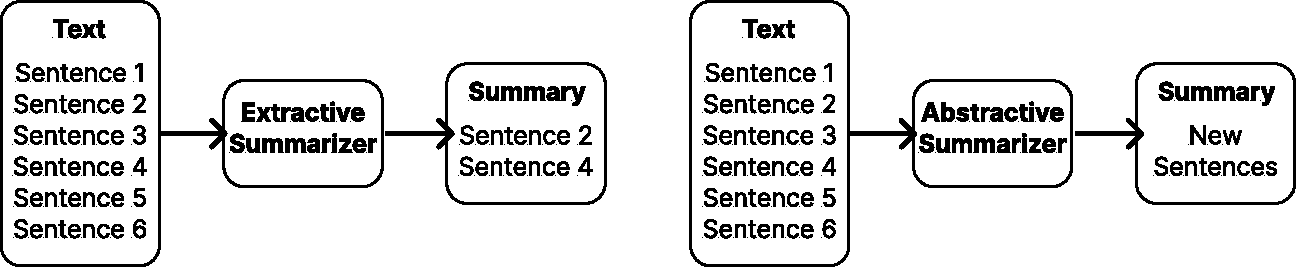
\includegraphics[width=0.8\linewidth]{Images/Extractive text summarizer and Abstractive text summarizer.pdf}\\
    \caption{Extractive and Abstractive text summarizer \cite[S.3]{yadav2022automatictextsummarizationmethods}}
    \label{fig:Extractive text summarizer and Abstractive text summarizer}
    \end{figure}

    
    \item[Die \ac{LLM}s] stehen durch das Wachstum des Internets große Informationsmengen zur Verfügung. Sie können kurze Zusammenfassungen von Quelltexten erstellen, ohne den Gesamtzusammenhang zu verlieren. Allerdings muss man bei der Verwendung von \ac{LLM}s vorsichtig sein und den Output kontrollieren, da zum Beispiel Halluzinationen auftreten können. Unter Halluzinationen versteht man Ausgaberesultate von \ac{LLM}s, die weder real noch im gelernten Datensatz enthalten sind. \cite[S.1]{banerjee2023benchmarkingllmpoweredchatbots}

    In Fisher's \ac{LLM} Comparison Research zeigt sich, dass \ac{LLM}s eine Möglichkeit bieten, Zeit zu sparen. Dennoch ist es notwendig, dass jemand die generierten Daten überprüft \cite{fisher2024large}. Es zeigt sich auch, dass \ac{LLM}s noch nicht an von Menschen geschriebene Texte heranreichen. Denn die von \ac{LLM}s generierten Texte sind umfangreich, folgen einer logischen Struktur und wiederholen sich häufig. Im Gegensatz dazu ist menschliches Schreiben vielfältig und unterschiedlich, da jeder Mensch eine andere Art hat, sich auszudrücken. Es wurde jedoch festgestellt, dass sich \ac{LLM}s ebenso wie menschliche Autoren voneinander unterscheiden \cite{rosenfeld2024whose}. Es bleibt abzuwarten, ob \ac{LLM}s in Zukunft so sprachgewandt werden wie Menschen.

     Ein weiterer interessanter Aspekt im Zusammenhang mit der Entwicklung von Prompts für \ac{LLM}s ist der von Levi und Neumann getestete Jailbreak-Angriff. Diese Attacke zielt darauf ab, den Sicherheitsmechanismus eines Sprachmodells zu umgehen. Dabei werden gezielt unauffällige Wörter oder Trennzeichen in Prompts eingefügt, um unerwünschte oder gefährliche Antworten zu provozieren. Selbst scheinbar harmlose Veränderungen des Prompts können das Verhalten des Modells erheblich beeinflussen \cite{levi2024vocabularyattackhijacklarge}. Die Sicherheit von \ac{LLM}s spielt daher heute eine zentrale Rolle, insbesondere bei der Entwicklung von Modellen für die breite Öffentlichkeit.
    
    \item[LaTeX] ist ein Textsatzsystem, das vor allem in wissenschaftlichen Kreisen zur Erstellung von Dokumenten verwendet wird. Es bietet erweiterte Funktionen für die Darstellung komplexer mathematischer Formeln und Referenzierungen. Die Verwendung von LaTeX ermöglicht eine präzise Kontrolle über das Layout und die Formatierung, was besonders bei umfangreichen Dokumenten von Vorteil ist.

    Aktuelle Entwicklungen in LaTeX zielen darauf ab, die Zugänglichkeit und Wiederverwendbarkeit eines \ac{PDF} zu verbessern, um Standards wie \ac{PDF}/\ac{UA} zu erfüllen. Diese Entwicklungen sind bereits seit einigen Jahren im Gange und 2024 wurde ein Prototyp erstellt, der diesen Standards entspricht.  \cite{mittelbach2024accessible}
    
    \item[\ac{DOCX}] ist eines der am weitesten verbreiteten Formate zur Erstellung und Bearbeitung von Textdokumenten. Es bietet eine breite Palette an Funktionen für Textformatierung, Multimedia-Integration und Layoutgestaltung.
    
    Eine der neuesten Funktionen von \ac{DOCX} ist die Integration von Copilot. Copilot ist eine \ac{KI}, die Benutzer beim Entwerfen und Schreiben von Dokumenten unterstützt. Sie bietet Möglichkeiten, Texte in Tabellen umzuwandeln, Texte umzuschreiben und mit dem Benutzer in einem interaktiven Chat zu kommunizieren. Zudem kann Copilot auch Zusammenfassungen generieren, was den Schreibprozess erleichtert. \cite{microsoft_copilot}
    
    \item[Die Web-Entwicklung]hat in den letzten Jahren bedeutende Fortschritte gemacht und ist zu einem der zentralen Bereiche der Informatik geworden. Insbesondere die Frontend-Entwicklung mit JavaScript-Frameworks wie React, Angular und Vue.js wird immer beliebter. Die Analyse von Vyas zeigt, dass React mit 35,9\% der Entwickler derzeit das beliebteste Framework ist. Außerdem zeigt Vyas mit Hilfe von Google Trends, dass React ein stabiles Wachstum aufweist, während Angular leicht rückläufig ist und Vue nur langsam wächst. \cite{vyas2022comparative} 
    
\end{description}

\section{Verwandte Webanwendungen}
In diesem Abschnitt werden verwandte Webanwendungen vorgestellt, welche ähnlich wie \textit{Reforge} mit \ac{KI} arbeiten und ebenfalls Zusammenfassungen generieren können. Sucht man im Browser nach Summary-Generatoren, so stößt man auf unzählige Seiten und Tools, die Texte zusammenfassen. Eine Handvoll dieser Tools wird näher betrachtet. Anschließend werden die Unterschiede des vorliegenden Projekts erläutert.

\begin{description}
    \item[Chat\ac{GPT}] ist ein \ac{KI}-basiertes Sprachmodell von OpenAI, das entwickelt wurde, um auf natürliche Weise mit Benutzern zu interagieren. Es ermöglicht beispielsweise das Schreiben von Texten, das Erlernen neuer Konzepte und das Sammeln von Ideen. In der mobilen Anwendung kann der Benutzer sogar eine Sprachkonversation starten. Außerdem können Antworten mit Links zu relevanten Webquellen abgerufen werden. Darüber hinaus bietet Chat\ac{GPT} die Möglichkeit, Dateien hochzuladen, um sie zu analysieren oder zusammenzufassen. Chat\ac{GPT} verfügt also über eine Vielzahl von Funktionen. \cite{openai_overview}

    \item[Microsoft Copilot] ist ein von Microsoft entwickelter \ac{KI}-Assistent, der sogar in Microsoft 365-Anwendungen integriert ist. Mit Hilfe von generativer \ac{KI} kann Copilot Inhalte erstellen und Daten analysieren. Er bietet auch eine Chat-Funktion, über die Nutzer Anweisungen an Copilot übermitteln können. \cite{microsoft_copilot_overview}

    \item[Google Gemini] ist eine von Google entworfene Chat-Anwendung mit künstlicher Intelligenz. Es hilft Nutzern bei Aufgaben wie Schreiben, Planen und Lernen. Durch die Eingabe von Textbefehlen können Nutzer direkt mit der \ac{KI} interagieren und erhalten passende Antworten. Gemini nutzt Informationen aus verschiedenen Quellen, einschließlich anderer Google-Dienste, um hilfreiche Antworten zu liefern. \cite{Gemini_overview}

    \item[Quillbot] ist ein \ac{KI}-gestütztes Schreibwerkzeug, das als Chrome-Erweiterung verfügbar ist. Es unterstützt den Benutzer bei der Verbesserung von Texten durch Funktionen wie Paraphrasierung, Grammatikprüfung und Tonerkennung. Darüber hinaus bietet es weitere Funktionen wie die Erstellung von Zusammenfassungen\footnote[1]{Quillbot: \href{https://quillbot.com/summarize}{https://quillbot.com/summarize}}. Außerdem bietet die Erweiterung sowohl kostenlose als auch kostenpflichtige Funktionen, um den unterschiedlichen Bedürfnissen der Nutzer gerecht zu werden.
    
\end{description}

\subsubsection{Unterscheidungsmerkmale von \textit{Reforge}}

Zusammenfassend unterscheidet sich das vorliegende Projekt von den genannten Lösungen durch folgende Eigenschaften:

\begin{itemize}
    \item \textit{Reforge} bietet keine Chat-Funktion, sondern nur Parameterfelder, die ausgefüllt werden müssen. Nach der Eingabe wird die Verarbeitung der Eingaben ähnlich wie bei Quillbot über einen Button gestartet.
    \item Ein wesentlicher Unterschied besteht in der Ausgabe. Der Nutzer kann wählen, ob er die Ausgabe als IEEEtran oder als OTH-Forschungsbericht erhalten möchte. Außerdem kann entschieden werden, ob der Technische Bericht in deutscher oder englischer Sprache erhalten werden soll. Diese Ausgabeparameter sind bei den genannten Werkzeugen nicht vorhanden.
    \item Das System bietet eine automatisierte Zusammenfassung von LaTeX-ZIP-Archive und \ac{DOCX}-Dokumenten mit Hilfe von \ac{LLM}s. Der Benutzer muss nicht wie bei ChatGPT oder Copilot Prompts an den \ac{LLM} senden.
\end{itemize}

Dieses Projekt stellt somit eine innovative Lösung zur Generierung von technischen Berichten aus LaTeX- oder \ac{DOCX}-Dokumenten dar. Der Benutzer ist flexibel und kann die gewünschte Ausgabe anpassen.
  \chapter{Konzeption und Entwurf von Reforge}
\section{Anforderungsanalyse}
Eine Anforderungsanalyse ist ein essenzieller Schritt im Entwicklungsprozess von Softwareprojekten. Sie stellt sicher, dass alle notwendigen Anforderungen erfasst, dokumentiert und verstanden werden, bevor mit der eigentlichen Entwicklung begonnen wird. Im Rahmen dieses Projekts wird das Modell der Anforderungsanalyse nach Kleuker herangezogen. \cite[S.51 ff.]{kleuker2013anforderungsanalyse}

\subsection{Funktionale Anforderungen}
\label{subs:funktionaleAnfoderungen}
 Funktionale Anforderungen werden üblicherweise durch die Modalverben „muss“, „soll“ und „wird“ klassifiziert, die den Erfüllungsgrad der jeweiligen Anforderung definieren. Anforderungen von wichtiger Bedeutung für das System werden mit „muss“ beschrieben, da deren Erfüllung für den Projekterfolg unverzichtbar ist. Anforderungen, die als hilfreich oder wünschenswert gelten, jedoch nicht zwingend erforderlich sind, werden mit „soll“ gekennzeichnet. Anforderungen, die als potenzielle Erweiterungen für die Zukunft betrachtet werden, werden mit „wird“ formuliert. Im Folgenden werden alle funktionalen Anforderungen des Projekts \textit{Reforge} nach dieser Klassifizierung beschrieben. \cite[S.71 ff.]{kleuker2013anforderungsanalyse}

 Des Weiteren werden, ähnlich zu Raus Vorgehensweise, für die einzelnen Anforderungen Akzeptanzkriterien formuliert, um diese präziser zu definieren. Ein Akzeptanzkriterium ist eine spezifische Bedingung, die erfüllt sein muss, damit eine Anforderung als vollständig umgesetzt gilt. \cite[S.49]{rau2016agile}

\subsubsection{A1 DOCX- und LaTeX-Input}

A1.1 Textextraktion: Das Programm muss in der Lage sein, den Textinhalt aus den hochgeladenen Dokumenten zu extrahieren. Es werden nur Abschlussarbeiten im DOCX-Format oder als LaTeX-ZIP-Ordner entgegengenommen. Die LaTeX-ZIP-Ordner müssen zudem eine Hauptdatei enthalten. Damit wird sichergestellt, dass der Text für die weitere Bearbeitung zur Verfügung steht. Diese Anforderung gilt als erfüllt, wenn der extrahierte Text den gesamten Inhalt des Dokuments umfasst und keine wesentlichen Teile auslässt.
 
\subsubsection{A2 \ac{LLM} Textzusammenfassung}
Die Anforderungen in „\ac{LLM} Textzusammenfassung“ umfasst mehrere Funktionen, die sicherstellen, dass Texte von dem \ac{LLM} verarbeitet und zusammengefasst werden können.

A2.1 Zusammenfassung-Generator: Das Programm muss mithilfe eines \ac{LLM}s in der Lage sein, eine Zusammenfassung der hochgeladenen Inhalte zu generieren. Das Akzeptanzkriterium dieser Anforderung ist erfüllt, wenn die generierten Zusammenfassungen die Hauptaussagen des Originaldokuments widerspiegeln.

A2.2 Textaufteilung zur Vermeidung von Token-Limits: Das Programm muss in der Lage sein, große Textmengen in kleinere Segmente aufzuteilen und diese nach der Verarbeitung wieder zu einem vollständigen Text zusammenzufügen. Diese Anforderung gilt als akzeptiert, wenn der Prozess der Aufteilung und Zusammenführung die inhaltliche Reihenfolge des ursprünglichen Textes nicht verändert. Außerdem muss die Segmentierung für sowohl \ac{DOCX} als auch LaTeX funktionieren.

A2.3 \ac{API}-Schnittstelle für \ac{LLM}: Das Programm muss in der Lage sein, mit der OpenAI-\ac{API} zu kommunizieren. Das Akzeptanzkriterium dieser Anforderung ist erfüllt, wenn die Anwendung eine stabile Verbindung zur OpenAI-\ac{API} aufbauen kann und Anfragen ohne Fehler übermitteln kann.

\subsubsection{A3 \ac{DOCX}- und LaTeX-Output}
Die Anwendung bietet zwei Exportfunktionen für die Ausgabe des generierten Textes. Sie bietet die Konvertierung in ein Word-Dokument und in ein LaTeX-Dokument.

A3.1 \ac{DOCX}-Ausgabe: Die Anwendung muss den generierten Text in das .docx-Format konvertieren können und dabei die Forschungsbericht-Vorlage verwenden. Als Akzeptanzkriterium wird sichergestellt, dass der entstandene Text in Microsoft Word fehlerfrei lesbar und editierbar ist. 

A3.2 LaTeX-Ausgabe: Die Anwendung muss den generierten Text zu .tex konvertieren können und dabei die IEEEtran-Vorlage berücksichtigen. Diese Anforderung gilt als akzeptiert, sobald das entstandene .tex-Dokument fehlerfrei kompilierbar ist.

\subsubsection{A4 Multi-lingual (EN/DE)}
A4.1 Sprachauswahl: Der Benutzer muss auswählen können, in welcher Sprache der Bericht erstellt wird. Diese Auswahl muss unabhängig von der Eingabesprache des Inputs erfolgen. Diese Anforderung gilt als akzeptiert, wenn der Nutzer eine Sprachauswahl tätigen kann.

A4.2 Automatische Übersetzung: Die Anwendung muss eine automatisierte Übersetzungsfunktion für englische und deutsche Versionen des Techreports haben. Sobald die vom Benutzer gewählte Sprache im generierten Endprodukt vorliegt, ist diese Anforderung erfüllt.

\subsubsection{A5 Sonstige funktionale Anforderungen}
A5.1 Benutzeroberfläche: Die Anwendung muss einen Upload-Bereich für die Dokumente haben. Die Anwendung muss Eingabefelder für die Report-Metadaten wie Titel, Autor und Datum haben. Die Anwendung muss eine Auswahl der Ausgabeformate und der gewünschten Sprache haben. Das Akzeptanzkriterium dieser Anforderung ist erfüllt, wenn alle Oberflächenelemente funktionsfähig sind.
    
A5.2 Fortschrittsanzeige: Die Anwendung soll den Fortschritt während der Textverarbeitung und des Exports anzeigen. Diese Anforderung gilt als erfüllt, sobald eine Fortschrittsanzeige zu sehen ist.

A5.3 Export-Funktion: Die Anwendung muss die Möglichkeit bieten, die generierten Berichte herunterzuladen. Das Akzeptanzkriterium dieser Anforderung ist erfüllt, wenn ein Dokument erfolgreich lokal gespeichert werden konnte.

A5.4 Fehlerbehandlung: Die Anwendung sollte auf Fehlersituationen wie ungültige Dateiformate oder \ac{API}-Ausfälle reagieren und dem Benutzer entsprechende Meldungen anzeigen. Diese Anforderung gilt als akzeptiert, wenn der Benutzer in der Lage ist Fehler-Rückmeldungen zu sehen.

\subsection{Nicht-Funktionale Anforderungen}
Die nicht-funktionalen Anforderungen sind entscheidend dafür, dass ein funktionstüchtiges und benutzerfreundliches Software-Projekt entsteht, das den Qualitätsstandards entspricht. \cite[S.77]{kleuker2013anforderungsanalyse}

Zur Klassifikation der nicht-funktionalen Anforderungen wird das FURPS-Modell herangezogen. FURPS steht dabei für Funktionalität, Usability, Reliability, Performance und Supportability. \cite{jamwal2010analysis}

Die Funktionalität umfasst Funktionen des Systems und Sicherheitsvorkehrungen:
\begin{itemize}
    \item Plattformunabhängigkeit: Die Anwendung sollte auf verschiedenen Betriebssystemen und in allen gängigen Webbrowsern konsistent funktionieren.
    \item Responsive Design: Die Benutzeroberfläche sollte sich dynamisch an verschiedene Bildschirmgrößen anpassen und sowohl auf Desktops als auch auf mobilen Geräten gut nutzbar sein.
\end{itemize}

Die Usability fokussiert sich auf die Benutzerfreundlichkeit:
\begin{itemize}
    \item Intuitive Benutzeroberfläche: Die Anwendung sollte einfach und intuitiv zu bedienen sein. Die wichtigsten Funktionen wie zum Beispiel der Upload sollten leicht zugänglich sein.
    \item Fehlermeldungen: Die Anwendung sollte verständliche Fehlermeldungen haben, welche dem Benutzer Hinweise geben, wie Fehler behoben werden können.
\end{itemize}

Die Reliability bezieht sich auf die Zuverlässigkeit des Systems:
\begin{itemize}
    \item Fehlertoleranz: Die Anwendung sollte in der Lage sein, bei einzelnen Fehlern wie zum Beispiel falsche Benutzereingaben weiterzufunktionieren.
    \item \ac{LLM} Verbindungsfehler: Die Anwendung sollte den Benutzer informieren, wenn die Verbindung zur \ac{LLM} im Backend fehlschlägt.
\end{itemize}

Die Performance beschreibt Anforderungen an Geschwindigkeit und Effizienz:
\begin{itemize}
    \item Reaktionszeit: Die Anwendung sollte in der Lage sein, Dokumente schnell zu verarbeiten und Zusammenfassungen in höchstens einer Minute zu generieren.
    \item Effiziente Verarbeitung: Trotz der Arbeit mit großen Textdokumenten sollte die Anwendung so optimiert sein, dass sie effizient mit Ressourcen wie Speicher umgeht.
\end{itemize}

Die Supportability definiert die Wartbarkeit und Erweiterbarkeit des Systems:
\begin{itemize}
    \item Zukünftige Formate: Die Architektur der Anwendung sollte so gestaltet sein, dass leicht neue Exportformate oder Vorlagen hinzugefügt werden können, ohne große Änderungen am bestehenden System vorzunehmen.
    \item \ac{API}-Erweiterbarkeit: Die Integration neuer \ac{API}s, zum Beispiel für Übersetzungen oder andere \ac{LLM}-\ac{API}s, sollte leicht möglich sein.
\end{itemize}
\section{Wireframes}
\label{sec:wireframe}
Ein wichtiges Mittel des Prototypings ist die Erstellung eines Wireframes. Ein Wireframe ist eine vereinfachte grafische Darstellung der Benutzeroberfläche einer Anwendung. Wireframes werden verwendet, um die grundlegende Struktur und Funktionalität einer Website oder Anwendung vor dem eigentlichen Design und der Implementierung zu visualisieren. Sie zeigen, wie Informationen angeordnet sind, welche Elemente auf der Benutzeroberfläche vorhanden sind und wie die Navigation im System funktioniert. Wireframes helfen, Ideen zu kommunizieren, Feedback von Nutzern oder Stakeholdern einzuholen und sicherzustellen, dass das Layout der Benutzeroberfläche den Anforderungen entspricht. \cite[S.119]{preim2015interaktive}

Die Abbildung \ref{fig:wireframe_upload} zeigt den Entwurf der Upload-Seite, in der alle wesentlichen Elemente skizziert sind. Zentrales Element der Seite ist der File-Upload-Button, über den die Benutzer ihre Dokumente hochladen können. Direkt darunter befinden sich die Eingabefelder für Autor und Titel, mit denen das generierte Dokument beschriftet wird. Es folgen Radiobuttons zur Auswahl des Ausgabeformats, wobei der Nutzer zwischen LaTeX und \ac{DOCX} wählen kann. Daneben ist eine Sprachauswahl eingebettet, die ebenfalls über Radiobuttons gesteuert wird und zwischen Deutsch und Englisch unterscheidet. Schließlich gibt es noch einen Start-Button, mit dem der Benutzer die Generierung des Berichts startet. Die Elemente wurden so angeordnet, dass die Seite wie ein Formular aussieht, das von oben nach unten ausgefüllt werden muss. 

\begin{figure}[H]
\centering
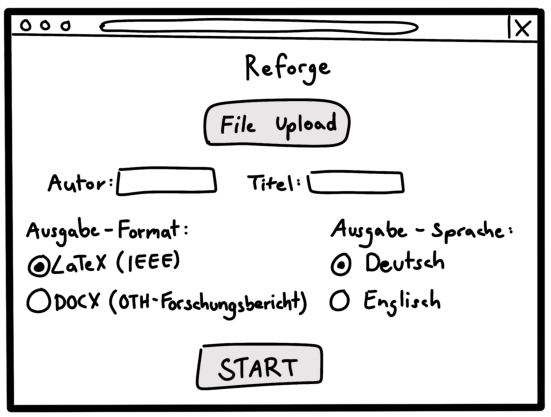
\includegraphics[width=0.5\linewidth]{Images/wireframe_upload.pdf}\\
\caption{Wireframe für die Upload-Seite von Reforge}
\label{fig:wireframe_upload}
\end{figure}

Die Abbildung \ref{fig:wireframe_download} zeigt die Hauptfunktionen der Download-Seite, die sich in zwei Buttons zusammenfassen lassen. Der eine Button ist für das Herunterladen der generierten Datei zuständig. Mit dem anderen Button kehrt der Benutzer zur Upload-Seite zurück, falls er sich entscheidet, einen weiteren Bericht zu generieren. Diese beiden Wireframes bilden eine gute Grundlage für die Entwicklung und stellen sicher, dass die Anordnung der Elemente optimal geplant wird.

\begin{figure}[H]
\centering
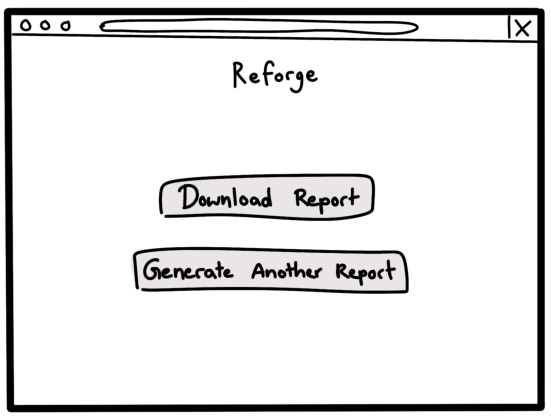
\includegraphics[width=0.5\linewidth]{Images/wireframe_download.pdf}\\
\caption{Wireframe für die Download-Seite von Reforge}
\label{fig:wireframe_download}
\end{figure}

\section{Auswahl des LLMs für die Textzusammenfassung}
\label{4.3_LLM}
Die Auswahl eines geeigneten \ac{LLM}s für die Textzusammenfassung ist ein wesentlicher Schritt, um die Qualität der erzeugten Berichte zu gewährleisten. Für dieses Projekt wurde das von OpenAI entwickelte \ac{GPT}-3.5-turbo ausgewählt, da dieses \ac{LLM} entscheidende Vorteile gegenüber anderen \ac{LLM}s bietet.

Ein großer Vorteil ist, dass die \ac{LLM}s von OpenAI nicht selbst gehostet werden müssen. Dies erleichtert die Integration der \ac{LLM}s in das System. Zudem verfügt OpenAI über eine gut dokumentierte \ac{API}, die sich leicht in die bestehende Systemarchitektur integrieren lässt, was die Entwicklungszeit verkürzt. Darüber hinaus zeichnen sich die von OpenAI entwickelten Modelle durch Präzision und ein tiefes Verständnis komplexer Textstrukturen aus. Sie ermöglichen die Erstellung von kontextbezogenen Zusammenfassungen, was insbesondere bei der Verarbeitung wissenschaftlicher Texte eine große Rolle spielt. 

OpenAI beschreibt in der Dokumentation, wie ein REST-\ac{API}-Aufruf gestaltet werden kann. Dieses Beispiel aus der offiziellen OpenAI Dokumentation ist in Listing \ref{lst:OpenAI_API_Example} dargestellt. Hier ist zu sehen, dass im \ac{API}-Request ein Modell definiert werden muss. OpenAI bietet viele verschiedene \ac{LLM}s an, die alle unterschiedliche Stärken und Schwächen besitzen. Eine Übersicht aller aktuell von OpenAI angebotenen Modelle ist auf der offiziellen Webseite\footnote[1]{OpenAI Modell Übersicht: \href{https://platform.openai.com/docs/models}{https://platform.openai.com/docs/models}} zu finden. Darunter ist das \ac{GPT}-4o-mini Model zu finden, welches hier in diesem Beispiel von OpenAI verwendet wird. Dieses Modell zeichnet sich damit aus günstig und schnell für kleinere Aufgaben zu sein. 

\begin{listing}[H]
\begin{minted}[
frame=lines,
bgcolor=base,
fontsize=\footnotesize,
linenos
]
{javascript}
import OpenAI from "openai";
const openai = new OpenAI();

const completion = await openai.chat.completions.create({
    model: "gpt-4o-mini",
    messages: [
        { role: "system", content: "You are a helpful assistant." },
        {
            role: "user",
            content: "Write a haiku about recursion in programming.",
        },
    ],
});

console.log(completion.choices[0].message);
\end{minted}
\caption{OpenAI REST-\ac{API}-Example \cite{openai_quickstart}}
\label{lst:OpenAI_API_Example}
\end{listing}

Als nächstes muss eine Nachricht, der sogenannte Prompt, definiert werden, welche das \ac{LLM} bei der Bearbeitung der Anfragen unterstützt. Diese Nachricht ist in mehrere Rollen unterteilt. Es gibt die \texttt{system}-Rolle, die dem \ac{LLM} Anweisungen gibt, was es erledigen und wie es reagieren soll. Die \texttt{user}-Rolle beschreibt, was der Output sein soll. Diese Rolle ist vergleichbar mit dem Benutzer im Chat\ac{GPT}, der im Chat eingibt, was er als Ergebnis haben möchte. \cite{openai_quickstart}

Im Vergleich dazu sind andere Modelle, wie die von Hugging Face angebotenen \ac{LLM}s, zwar ebenfalls leistungsfähig, erfordern aber oft eine umfangreiche Feinabstimmung und eine eigene Hosting-Infrastruktur, was den Aufwand für das Projekt erhöht hätte. Die Entscheidung für OpenAI basierte daher auf einer Abwägung zwischen einfacher Integration, hoher Sprachqualität und möglichst effizienter Entwicklungszeit.


\section{Systemarchitektur}

In diesem Abschnitt wird zunächst die Architektur des Systems erläutert. Anschließend wird auf die Speicherung der Daten eingegangen. Schließlich wird ein Sequenzdiagramm vorgestellt, welches den Upload Ablauf visualisiert.

\begin{figure}[H]
\centering
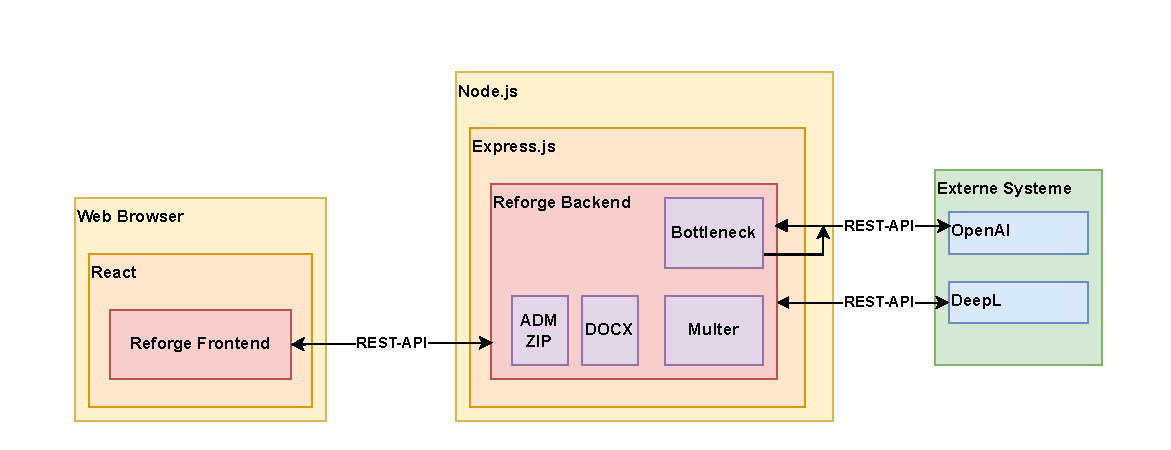
\includegraphics[width=1\linewidth]{Images/Systemarchitektur.pdf}\\
\caption{Systemarchitektur von Reforge}
\label{fig:sys_architektur}
\end{figure}

Die Abbildung \ref{fig:sys_architektur} zeigt den Entwurf für die Systemarchitektur der Anwendung Reforge. Diese Architektur setzt auf eine RESTful \ac{API}, die eine Kommunikation zwischen Frontend, Backend und den externen Systemen ermöglicht. Dabei werden Daten über \ac{HTTP}-Methoden wie \textbf{POST} ausgetauscht.

Das Frontend basiert auf React und läuft im Webbrowser des Benutzers. Es stellt die Benutzerschnittstelle bereit, über die alle Interaktionen erfolgen. Die Benutzereingaben werden über die RESTful \ac{API} an das Backend übertragen. 

Das Backend, ausgeführt mit Node.js und Express.js, übernimmt die serverseitige Logik und verarbeitet die Anfragen, die vom Frontend gesendet werden. Die Verwaltung der Dateispeicherung erfolgt mithilfe von Middleware wie Multer \footnote[1]{Multer: \href{https://expressjs.com/en/resources/middleware/multer.html}{https://expressjs.com/en/resources/middleware/multer.html}}, das die Daten temporär im Arbeitsspeicher zwischenspeichert, bevor sie weiterverarbeitet werden. Für das Management und die Verarbeitung von Dateien verwendet das Backend ADM-ZIP\footnote[2]{ADM-ZIP: \href{https://www.npmjs.com/package/adm-zip}{https://www.npmjs.com/package/adm-zip}} für das Handling von ZIP-Dateien sowie DOCX\footnote[3]{DOCX: \href{https://www.npmjs.com/package/docx}{https://www.npmjs.com/package/docx}} zur Formatierung und Erstellung von Word-Dokumenten. Diese Tools ermöglichen es dem Backend, die hochgeladenen Inhalte im gewünschten Format bereitzustellen.

Zur Erweiterung der Funktionalität greift die Anwendung auf externe Systeme zurück. Die OpenAI \ac{API}\footnote[4]{OpenAI API: \href{https://platform.openai.com/docs/overview}{https://platform.openai.com/docs/overview}} wird für die Verarbeitung und Generierung von Textinhalten genutzt, während die DeepL \ac{API}\footnote[5]{DeepL API: \href{https://www.deepl.com/de/pro-api/}{https://www.deepl.com/de/pro-api/}} die Übersetzung von Überschriften innerhalb der Anwendung übernimmt. Da OpenAI bei zu vielen Anfragen in kurzer Zeit blockiert, wird Bottleneck\footnote[6]{Bottleneck: \href{https://www.npmjs.com/package/bottleneck}{https://www.npmjs.com/package/bottleneck}} eingesetzt, um die Anfragerate für die OpenAI \ac{API} gezielt zu drosseln.

\subsection{Speicherung von Daten}
Im Rahmen dieses Projekts wurde bewusst darauf verzichtet, eine Datenbank zu implementieren, da dies nicht Teil der Anforderungen war und den Projektrahmen gesprengt hätte. Stattdessen erfolgt die Speicherung der Daten aktuell nur in Form einer temporären Zwischenspeicherung innerhalb der Anwendung.

Für die Zwischenspeicherung kommt die Middleware Technologie Multer zum Einsatz, die es ermöglicht, hochgeladene Dateien für die Dauer der Verarbeitung zu speichern und anschließend weiterzuleiten. Hierfür wird die \textbf{memoryStorage}-Funktion von Multer verwendet, welche die Dateien als Buffer speichert. Bei dieser Methode enthält das Dateifeld ein Buffer-Objekt, welches die gesamte Datei im Arbeitsspeicher hält. Diese Vorgehensweise ist effizient für kleinere Dateien. Der Arbeitsspeicher kann jedoch bei großen oder sehr vielen kleinen Dateien überlastet werden, weshalb die Speicherlast im Auge behalten werden sollte. \cite{multer}

\subsection{Verlauf des Uploads in Reforge}

Um die zeitliche Abfolge von Interaktionen zwischen den Komponenten eines Systems darzustellen, eignet sich das Sequenzdiagramm. Es gehört zu den Verhaltensdiagrammen der \ac{UML} und ist eines der vier Interaktionsdiagramme. Sequenzdiagramme zeigen, wie die Kommunikation zwischen verschiedenen Systemkomponenten abläuft, indem sie die gesendeten Nachrichten und deren zeitliche Reihenfolge veranschaulichen \cite{rumpe2004sequenzdiagramme}. Mit Hilfe von einem Sequenzdiagrammen soll nun der Prozess des Uploadens von Dateien erklärt werden.

Abbildung \ref{fig:Sequenzdiagramm} zeigt das Sequenzdiagramm des Upload-Prozesses in der Anwendung. Der Ablauf beginnt im Frontend, wo der Benutzer eine Datei hochlädt. Das Backend empfängt die Datei, liest sie und bereitet den Text für die weitere Verarbeitung vor. Anschließend wird der vorbereitete Text an die OpenAI \ac{API} gesendet, um eine Zusammenfassung zu generieren. Sobald die Zusammenfassung erstellt wurde, kehrt diese zum Backend zurück. Danach wird der Text an die Deepl \ac{API} gesendet, um die Überschriften zu übersetzen. Die übersetzten und verarbeiteten Daten werden schließlich an das Frontend zurückgesendet, sodass die fertige Datei dem Benutzer zur Verfügung gestellt werden kann.

\begin{figure}[H]
\centering
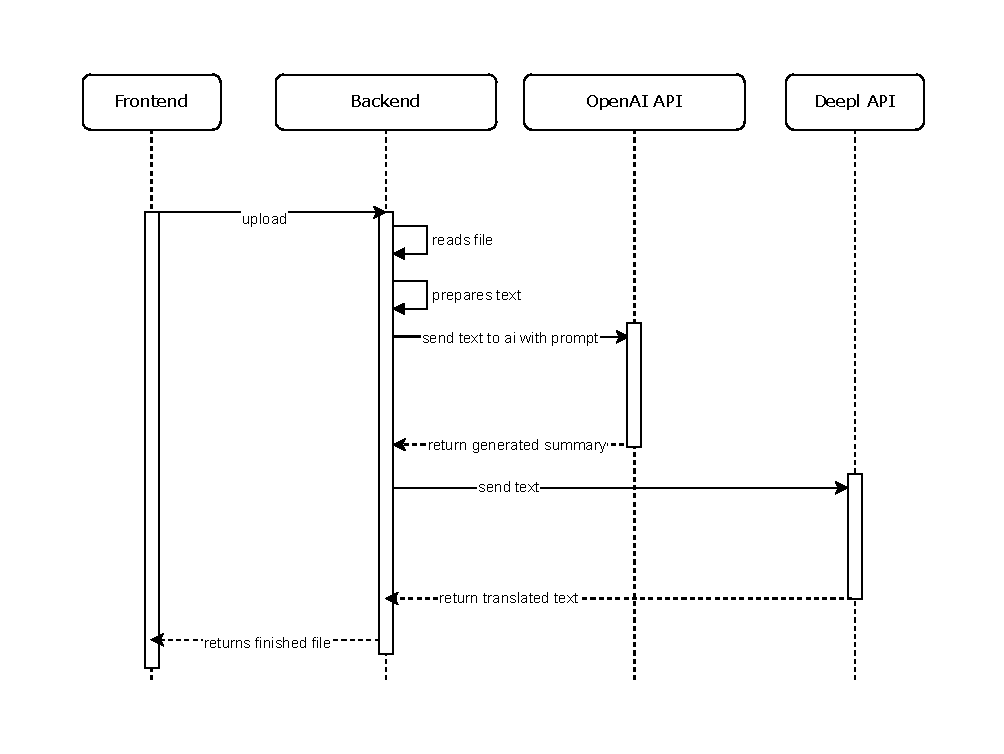
\includegraphics[width=1\linewidth]{Images/Sequenzdiagramm.pdf}\\
\caption{Sequenzdiagramm des Upload-Prozesses}
\label{fig:Sequenzdiagramm}
\end{figure}



  \chapter{Implementierung von Reforge}

\section{Entwicklung des Backends}
Das Backend von \textit{Reforge} ist für die Verarbeitung der hochgeladenen Dateien und die Generierung der technischen Berichte verantwortlich. 


\subsection{Kommunikation zwischen Frontend und Backend}
\label{subse:kommu_froback}

Es wird nun im folgendem die Kommunikation zwischen Frontend und Backend von \textit{Reforge} näher erläutert. Ziel dieser Kommunikation ist der Austausch von Daten und die Bereitstellung eines verarbeiteten Berichts als Datei-Download für den Benutzer. Der Ablauf erfolgt mit einer RESTful \ac{API}. Er wird erst gestartet, sobald der Nutzer im Frontend zum Beispiel einen LaTeX-ZIP-Ordner einfügt, alle nötigen Parameter ausfüllt und auf den Button \textbf{Start the generation} klickt.

Das Listing \ref{lst:Frontend_API_Aufruf} zeigt den Code für den Aufruf der RESTful \ac{API} im Frontend. Die \ac{URI} \texttt{http://localhost:5000/api/upload} verweist auf den Endpunkt des Backends, der für das Hochladen von Dateien zuständig ist. Die Anfrage wird als \ac{HTTP} \textbf{POST} gesendet, da Dateien und zusätzliche Parameter wie das gewünschte Format oder die Sprache übermittelt werden. Der Header \texttt{Content-Type} ist auf \texttt{multipart/form-data} gesetzt, um dem Server mitzuteilen, dass es sich um einen Datei-Upload handelt. Zusätzlich wird mit \texttt{responseType: 'blob'} spezifiziert, dass die Antwort vom Server als \ac{Blob} erwartet wird, was für den späteren Download des Berichts wichtig ist. Es dient unter anderem dazu, binäre Daten übertragbar zu machen. So ist es möglich, die Dateien später herunterzuladen.


\begin{listing}[H]
\begin{minted}[
frame=lines,
bgcolor=base,
fontsize=\footnotesize,
linenos
]
{typescript}
// API-Aufruf im Frontend
const response = await axios.post('http://localhost:5000/api/upload', formData, {
  headers: {
    'Content-Type': 'multipart/form-data',
  },
  responseType: 'blob',
});
\end{minted}
\caption{API POST Aufruf im Frontend}
\label{lst:Frontend_API_Aufruf}
\end{listing}

Nachdem das Backend die Anfrage erhalten hat, wird die hochgeladene Datei verarbeitet. Sobald das Backend alle Verarbeitungsschritte zur Erstellung des Berichts abgeschlossen hat, fügt es die neuen Informationen in den Header der Antwort ein. Der Statuscode 200 wird zurückgesendet, um anzuzeigen, dass die Anfrage des Frontends erfolgreich verarbeitet wurde. Gleichzeitig wird der zusammengesetzte Bericht mit dem Statuscode an das Frontend gesendet. Das folgende Listing \ref{lst:Backend_API_Antwort} zeigt, wie der Code dafür aussieht.

\begin{listing}[H]
\begin{minted}[
frame=lines,
bgcolor=base,
fontsize=\footnotesize,
linenos
]
{typescript}
// API-Antwort im Backend
    res.setHeader('Content-Disposition', `attachment; filename="${title}.tex"`);
    res.setHeader('Content-Type', 'text/plain');
    res.status(200).send(combinedReport);
\end{minted}
\caption{Zurücksendung der abgeschlossenen \ac{API}-Anfrage ans Frontend}
\label{lst:Backend_API_Antwort}
\end{listing}

Im Frontend wird die Antwort des Backends überprüft, wie in Listing \ref{lst:Frontend_API_Antwort} dargestellt. Bei einem Statuscode von \texttt{200} wird ein neues \texttt{\ac{Blob}}-Objekt erzeugt, das die empfangenen Binärdaten (\texttt{combinedReport}) enthält. Mithilfe von \texttt{window.URL.createObjectURL} wird eine \ac{URL} generiert, die es dem Benutzer ermöglicht, die Datei herunterzuladen.

\begin{listing}[H]
\begin{minted}[
frame=lines,
bgcolor=base,
fontsize=\footnotesize,
linenos
]
{typescript}
if (response.status === 200) {
  const url = window.URL.createObjectURL(new Blob([response.data]));
  setUploadStatus('File successfully uploaded.');

  navigate('/download', { state: { downloadUrl: url, title: title, format: format } });
} else {
  setUploadStatus('Error while uploading the file.');
}
\end{minted}
\caption{API Rückgabe Empfang im Frontend}
\label{lst:Frontend_API_Antwort}
\end{listing}

Die \ac{URL}-Generierung erfolgt dabei in mehreren Schritten. Zunächst wird das vom Backend empfangene Binärdatenobjekt als \texttt{\ac{Blob}} formatiert.  Anschließend wird mit \texttt{window.URL.createObjectURL(blob)} eine temporäre \ac{URL} erstellt, die im Browser als Verweis auf dieses \ac{Blob} dient. Diese \ac{URL} ist nur während der aktuellen Browsersitzung gültig und sieht beispielsweise so aus:

\texttt{blob:http://localhost:3000/3f9a8d7e-2b4c-48e6-a91f-bb23c1def456}. 

Nach der \ac{URL}-Erstellung wird der Benutzer auf eine neue Seite weitergeleitet, auf der er den Bericht herunterladen kann. Ist hingegen vorher ein Fehler aufgetreten, beispielsweise wenn das Backend einen anderen Statuscode zurückgibt, wird statt der Weiterleitung eine Fehlermeldung angezeigt.

Auf diese Weise wird die gesamte Kommunikation zwischen Frontend und Backend durch einen einzigen \textbf{POST}-Request ermöglicht. Das Frontend überträgt alle notwendigen Informationen an das Backend und wartet auf die Antwort. Nach erfolgreicher Verarbeitung stellt das Backend den generierten Bericht als Datei bereit, die im Frontend heruntergeladen werden kann. 

\subsection{Verwendete Backend Bibliotheken}
Die Backend-Entwicklung der Anwendung basiert auf einer Reihe von Bibliotheken, die die Verarbeitung von Daten, die Dateiverwaltung und die Bereitstellung der \ac{API}s unterstützen. Im Folgenden werden die verwendeten Bibliotheken aus dem Listing \ref{lst:Backend_Bibliotheken} und ihre Hauptfunktionen beschrieben.

\begin{listing}[H]
\begin{minted}[
frame=lines,
bgcolor=base,
fontsize=\footnotesize,
linenos
]
{typescript}
"dependencies": {
    "adm-zip": "^0.5.15",
    "bottleneck": "^2.19.5",
    "cors": "^2.8.5",
    "docx": "^8.5.0",
    "express": "^4.17.1",
    "jsdom": "^25.0.1",
    "multer": "^1.4.2"
}
\end{minted}
\caption{Backend Bibliotheken}
\label{lst:Backend_Bibliotheken}
\end{listing}

Die Bibliothek ADM-ZIP ermöglicht den einfachen Umgang mit ZIP-Dateien. Sie dient zum Erstellen, Entpacken und Lesen von ZIP-Archiven. Da in Reforge mit LaTeX-ZIP-Dateien gearbeitet wird, ist diese Bibliothek unverzichtbar.

Die Bottleneck-Bibliothek wird für die Verwaltung von Anforderungsraten verwendet. Sie hilft, die Anzahl der gleichzeitigen Anfragen an externe \ac{API}s zu kontrollieren, um eine Überlastung zu vermeiden.

Die CORS Bibliothek ermöglicht die Aktivierung von \ac{CORS}, um den Zugriff von Webanwendungen auf Serverressourcen zu kontrollieren. Dies ist notwendig, damit der Frontend-Client sicher auf die Backend-Ressourcen zugreifen kann.

Die \ac{DOCX}-Bibliothek wird zur Erzeugung von Word-Dokumenten verwendet. Sie ermöglicht es der Anwendung, Berichte im Word-Format zu erstellen und diese zu formatieren.

Express ist ein minimalistisches Web-Framework für Node.js, das die Entwicklung von Backend-Servern vereinfacht. Es bietet Funktionen zur Erstellung von \ac{API}s, die das Rückgrat der serverseitigen Logik bilden. Express stellt sicher, dass die Kommunikation zwischen Client und Server reibungslos verläuft.

Die jsdom-Bibliothek bietet eine JavaScript-Implementierung des \ac{DOM}. Sie ermöglicht das Parsen und Manipulieren von \ac{HTML} im Backend, was bei der Verarbeitung und Extraktion von Daten aus \ac{DOCX}-Dokumenten hilfreich ist.

Multer ist eine Middleware für Datei-Uploads. Sie wird verwendet, um die vom Benutzer hochgeladenen Dateien zur Verarbeitung entgegenzunehmen. Diese Dateien werden mit der Funktion \textbf{memoryStorage()} im Arbeitsspeicher zwischengespeichert. Diese Bibliotheken bilden die Grundlage für das Backend von \textit{Reforge}.

\subsection{LaTeX-ZIP-Verarbeitung}

In diesem Abschnitt werden die einzelnen Prozessschritte der LaTeX-ZIP-Verarbeitung erläutert. Im Listing \ref{lst:Entscheidung_ZIP_DOCX} ist zu sehen, wie das Backend zunächst prüft, ob es sich bei der hochgeladenen Datei um eine ZIP-Datei handelt. Abhängig davon wird hier entweder der ZIP-Prozess oder der \ac{DOCX}-Prozess gestartet.

\begin{listing}[H]
\begin{minted}[
frame=lines,
bgcolor=base,
fontsize=\footnotesize,
linenos
]
{typescript}
if (req.file.originalname.endsWith('.zip')) {
  combinedReport = await processZipFile(req.file, mainfile, author, language, format);
} else if (req.file.originalname.endsWith('.docx')) {
  combinedReport = await processDocxFile(req.file, author, language, format);
}
\end{minted}
\caption{Entscheidung zwischen der ZIP- oder \ac{DOCX}-Verarbeitung}
\label{lst:Entscheidung_ZIP_DOCX}
\end{listing}

LaTeX-Projekte sind häufig in mehrere Kapitel und Abschnitte unterteilt, die in separaten Dateien organisiert sind. Diese Struktur wird durch die Hauptdatei gesteuert, in der die einzelnen Kapiteldateien mittels \texttt{\textbackslash include\{\}}-Anweisungen eingebunden werden. Um die korrekte Reihenfolge der Kapitel für die Weiterverarbeitung zu haben, muss die Reihenfolge dieser \texttt{include}-Anweisungen aus der Hauptdatei entnommen werden. Damit die spätere Zusammenfassung in der richtigen Reihenfolge erfolgt, ist dieser Schritt unerlässlich.

Im Frontend fragt die Anwendung über einen Parameter den Namen der Hauptdatei des LaTeX-Ordners ab. Das Listing \ref{lst:Mainfile_Search} zeigt den Code für die Suche nach der Hauptdatei. Sobald also die Funktion \textbf{processZipFile} aufgerufen wird, wird zunächst geprüft, ob die angegebene Hauptdatei innerhalb des ZIP-Ordners gefunden werden kann. Wenn die Hauptdatei nicht gefunden werden kann, wird ein Fehler ausgegeben. Ist die Suche nach der Hauptdatei erfolgreich, wird mit der Funktion \textbf{getIncludeOrder} jede Include-Anweisung in einem String gespeichert. Außerdem wird hier die ADM-ZIP Bibliothek verwendet, um die ZIP-Inhalte zu durchsuchen und die Dateien zu entnehmen.

\begin{listing}[H]
\begin{minted}[
frame=lines,
bgcolor=base,
fontsize=\footnotesize,
linenos
]
{typescript}
  const zip = new AdmZip(file.buffer);
  const zipEntries = zip.getEntries();
  const path = require('path');
  let includeOrder: string[] = [];
  let mainFileFound = false;

  // Mainfile im zip finden
  for (const zipEntry of zipEntries) {
    const entryName = path.basename(zipEntry.entryName);
    
    // wenn mainfile gefunden -> hole include reihenfolge
    if (!zipEntry.isDirectory && entryName === mainfile) {
      mainFileFound = true; 
      const fileContent = zipEntry.getData().toString('utf-8');
      if (fileContent.includes('\\include{')) {
        includeOrder = getIncludeOrder(fileContent);
        break;
      }
    }
  }
  
  // error wenn mainfile nicht gefunden
  if (!mainFileFound) throw new Error(`Main file "${mainfile}" not found in ZIP`);
\end{minted}
\caption{Dieser Codeabschnitt sucht die LaTeX-Hauptdatei im ZIP-Ordner und holt sich die Include-Reihenfolge aus der Hauptdatei}
\label{lst:Mainfile_Search}
\end{listing}

\subsubsection{Die getIncludeOrder-Funktion}

Der folgende Code in Listing \ref{lst:getIncludeORder} zeigt die Implementierung der Funktion, welche die Include-Reihenfolge ausliest. Die Suche nach dem Inhalt erfolgt mit einem regulären Ausdruck, wobei der Inhalt zwischen den geschweiften Klammern \texttt{\{\}} des regulären Ausdrucks am wichtigsten ist, da wir diesen Inhalt für die Datei zusammenstellung benötigen. Dieser Part des Musters wird dementsprechend näher erläutert: \texttt{([\textasciicircum\}]+)}

\begin{listing}[H]
\begin{minted}[
frame=lines,
bgcolor=base,
fontsize=\footnotesize,
linenos
]
{typescript}
function getIncludeOrder(mainfile: string): string[] {
  const includePattern = /\\include\{([^}]+)\}/g;
  let match;
  const includeFiles: string[] = [];
  
  //suche nach Übereinstimmungen solange match !== null 
  while ((match = includePattern.exec(mainfile)) !== null) {
    //jedes gefundene include wird in den array gepushed
    includeFiles.push(match[1].trim());
  }

  return includeFiles;
}
\end{minted}
\caption{Funktion zur Extraktion der Include-Reihenfolge}
\label{lst:getIncludeORder}
\end{listing}

Für ein besseres Verständnis wird das Muster \texttt{([\textasciicircum\}]+)} in mehreren Teilen erklärt. Die eckigen Klammern \texttt{[\textasciicircum\}]} definieren eine Negation. Das \texttt{\textasciicircum} bedeutet \glqq nicht \grqq{}, also steht \texttt{[\textasciicircum\}]} für \glqq kein \}\grqq{}. Das Pluszeichen \texttt{+} bedeutet, dass mindestens ein oder mehrere Zeichen gefunden werden sollen, die nicht \texttt{\}} sind. Die runden Klammern \texttt{(...)} um \texttt{([\textasciicircum\}]+)} gruppieren diesen Teil und sorgen dafür, dass der Inhalt in einer sogenannten Capture Group gespeichert wird. Mit diesem Muster können alle Dateinamen innerhalb der Include-Klammer extrahiert werden.

Solange das Muster in der While-Schleife Übereinstimmungen findet, wird diese Übereinstimmung in einem String angelegt. Dazu wird mit \texttt{match[1]} auf den gefundenen Inhalt der Capture Group zugegriffen. Zusätzlich wird mit \texttt{trim()} sichergestellt, dass keine unerwünschten Leerzeichen enthalten sind.

\subsubsection{Kombinieren der Kapiteldateien}

Nachdem die Reihenfolge der Kapiteldateien ermittelt wurde, müssen die entsprechenden \texttt{.tex}-Dateien aus dem ZIP-Archiv geladen und in der richtigen Reihenfolge zusammengefügt werden. Das folgende Listing \ref{lst:Kombination der Kapiteldateien} zeigt, wie die Dateien aus dem ZIP-Archiv mit der erhaltenen Reihenfolge zusammengefügt werden.

\begin{listing}[H]
\begin{minted}[
frame=lines,
bgcolor=base,
fontsize=\footnotesize,
linenos
]
{typescript}
for (const fileName of includeOrder) {
  //hinzufügen von .tex  zur filename falls nicht vorhanden
  const texFileName = fileName.endsWith('.tex') ? fileName : `${fileName}.tex`;
  //finde texFileName im Zip
  const zipEntry = zipEntries.find(entry => entry.entryName.endsWith(texFileName));
  //prüfung ob datei existiert und kein verzeichnis ist
  if (zipEntry && !zipEntry.isDirectory) {
    //hole text inhalt
    let fileContent = zipEntry.getData().toString('utf-8');
    //sammlung von allen datei inhalten in allFileContent
    allFileContent += fileContent + '\n';
  }
}
\end{minted}
\caption{Kombination der Kapiteldateien}
\label{lst:Kombination der Kapiteldateien}
\end{listing}

Zunächst wird geprüft, ob der Dateiname die Endung \texttt{.tex} enthält. Falls nicht, wird diese angehängt, da in LaTeX-Dateien oft nur der Basisname im Include angegeben ist. Anschließend wird das ZIP-Archiv nach der entsprechenden Datei durchsucht. Wenn die Datei gefunden wird und es sich nicht um ein Verzeichnis handelt, wird ihr Inhalt ausgelesen und in der Variablen \texttt{allFileContent} gespeichert. Dieses Verfahren stellt sicher, dass die Kapiteldateien in der richtigen Reihenfolge kombiniert werden, so dass der gesamte Text des Dokuments vollständig rekonstruiert werden kann.

\subsubsection{LaTeX-Textfilter und Aufteilung}

Um sicherzustellen, dass nur die relevanten Teile eines LaTeX-Dokuments an die OpenAI-Schnittstelle für die Erstellung von Zusammenfassungen übergeben werden, ist es notwendig, den Text vorher zu bereinigen. Außerdem ist die Anzahl der übertragbaren Token begrenzt, so dass überflüssige LaTeX-Befehle, Kommentare und unnötige Leerzeichen aus dem Text entfernt werden müssen. Der Befehl \texttt{\textbackslash chapter} bleibt jedoch erhalten, da dieser für die spätere Aufteilung des Textes wichtig ist. Für die Filterung werden reguläre Ausdrücke verwendet, um LaTeX-Kommandos gezielt auszusortieren beziehungsweise beizubehalten. Ein Codeauszug der LaTeX-Filterfunktion ist im Anhang im Listing \ref{lst:LaTeX-Text-Filterung} zu finden. 

Auch nach der Filterung ist der Gesamttext noch zu lang, so dass eine sinnvolle Zerlegung des Dokuments notwendig ist. Damit die \ac{KI} sinnvolle Zusammenfassungen erstellen kann, ohne den Kontext zu verlieren, wird der Text mit Hilfe der \texttt{\textbackslash chapter}-Kommandos zerlegt. Aus diesem Grund wurden die \texttt{\textbackslash chapter}-Befehle vorher nicht herausgefiltert. Diese Vorgehensweise ermöglicht es, die begrenzte Anzahl von Token der OpenAI einzuhalten und dennoch einen zusammenhängenden Text für die Zusammenfassungen zu erzeugen. Die Kapitelaufteilung ist im Listing \ref{lst:Chapter_Mapping} in Zeile zwei dargestellt.

\begin{listing}[H]
\begin{minted}[
frame=lines,
bgcolor=base,
fontsize=\footnotesize,
linenos
]
{typescript}
//Zerstückelung des Textes bei Chapter
const chapters = allFileContent.split(/(?=\\chapter\{)/g);

//Alle Kapitel durchgehen & Bericht erstellen
const reportPromises = chapters.map((chunk) => {
  const chapternameMatch = chunk.match(/\\chapter\{([^}]+)\}/); 
  const chapterTitle = chapternameMatch ? chapternameMatch[1] : 'Unnamed Chapter'; 
    
  return LanguageDetection(chunk, language, author, format, 'tex').then((report) => {
    return `\\section{${chapterTitle}}\n${report}`;
  });
});
const reportParts = await Promise.all(reportPromises);
let combinedReport = reportParts.join('\n\n');
 
combinedReport = removeSpecialChars(combinedReport);
\end{minted}
\caption{Chapter-Mapping für die Textübertragung an OpenAI}
\label{lst:Chapter_Mapping}
\end{listing}

Darüber hinaus wird im Listing \ref{lst:Chapter_Mapping} ein Kapitel-Mapping durchgeführt, damit jedes einzelne Kapitel für die Zusammenfassungsgenerierung übergeben wird. Um sicherzustellen, dass die Kapitelnamen während des Prozesses nicht verloren gehen, werden diese zuvor mit einem regulären Ausdruck gesucht und in \texttt{ChapterTitle} abgelegt. Ist kein Titel vorhanden, wird der Textabschnitt mit \texttt{Unnamed Chapter} betitelt. In der Funktion \textbf{Language Detection} findet die Spracherkennung und die Kommunikation mit OpenAI statt. Diese Funktion wird im folgenden Abschnitt erläutert. Anschließend werden alle generierten Berichtsteile wieder in \texttt{combinedReport} zusammengeführt.

Es kann vorkommen, dass OpenAI bei der Generierung Sonderzeichen wie \& oder \% verwendet. Da LaTeX mit solchen Zeichen Fehler aufwirft, werden diese mit der Funktion \textbf{removeSpecialChars} nachträglich entfernt. Zusätzlich entfernt diese Funktion die ursprüngliche Nummerierung der Überschriften. Diese Funktion ist im Listing \ref{lst:SpecialChar-Filterung} im Anhang zu finden.

\subsubsection{Die LanguageDetection-Funktion}
Die von OpenAI generierten Texte wurden nicht immer zuverlässig in der richtigen Sprache zurückgegeben, obwohl im Prompt die gewünschte Sprache angegeben wurde. Um dieses Problem zu lösen, wurde eine Spracherkennung implementiert, welche die Sprache des generierten Textes mit der gewünschten Sprache vergleicht.

Das Listing \ref{lst:dowhile_LanguageDetection} zeigt den Teil der Funktion \textbf{Language Detection}, in dem eine Schleife ausgeführt wird, bis die erkannte Sprache im generierten Bericht mit der erwarteten Sprache übereinstimmt. Im Frontend kann der Benutzer auswählen, ob die Ausgabe in Englisch oder Deutsch erfolgen soll. Diese Auswahl wird als \textit{erwartete Sprache} definiert. Nur wenn die Sprachen übereinstimmen, wird der in \textbf{generateTechReport} erzeugte Bericht zurückgegeben. Die Spracherkennung erfolgt über die Funktion \textbf{detectLanguageUsingStopWords}, welche die Sprache der generierten Texte anhand von Stopwörtern überprüft. Wie die Spracherkennung mittels Stopwörtern funktioniert, wird im folgenden Abschnitt erläutert.

\begin{listing}[H]
\begin{minted}[
frame=lines,
bgcolor=base,
fontsize=\footnotesize,
linenos
]
{typescript}
do {
  summary = await generateTechReport(content, expectedLanguage, format, docType);

  detectedLanguage = detectLanguageUsingStopWords(summary);
    
  if (detectedLanguage.toLowerCase() !== expectedLanguage.toLowerCase()) {
    console.log(`Sprache nicht korrekt erkannt. Versuche erneut...`);
  }
} while (detectedLanguage.toLowerCase() !== expectedLanguage.toLowerCase());
  return summary;
}
\end{minted}
\caption{Do-While-Schleife der LanguageDetection-Funktion}
\label{lst:dowhile_LanguageDetection}
\end{listing}

\subsection{Spracherkennung mittels Stopwörtern}

Die Analyse von Stoppwörtern ist eine einfache Methode, um die Sprache eines Textes zu ermitteln. Stoppwörter sind Wörter, die in der natürlichen Sprache als wenig informativ gelten und häufig vorkommen. Sie können jedoch Hinweise auf die Sprache eines Textes geben, da ihre genaue Form von Sprache zu Sprache variiert.

Dunning hat gezeigt, dass statistische Methoden zur Spracherkennung eingesetzt werden können. Die Idee dahinter ist, dass man anhand der Verteilung von Zeichenketten feststellen kann, ob ein Text beispielsweise auf Deutsch oder Englisch verfasst wurde \cite{dunning1994statistical}. Bei diesem Ansatz werden statt Zeichenketten Stoppwörter verwendet, um die Sprachverteilung zu bestimmen.

\subsubsection{Warum sind Stopwörter nützlich für die Spracherkennung?}
\begin{itemize}
    \item \textbf{Hohe Häufigkeit und Sprachspezifität:}  
    Stopwörter treten in jedem Text häufig auf, ihre Form ist jedoch in jeder Sprache unterschiedlich. Beispielsweise kommen die deutschen Stopwörter \glqq der\grqq{}, \glqq die\grqq{}, \glqq das\grqq{} oft in deutschen Texten vor, während sie in englischen Texten fehlen. Umgekehrt finden sich englische Stopwörter wie \glqq the\grqq{}, \glqq and\grqq{}, \glqq is\grqq{} in fast jedem englischen Text.

    \item \textbf{Geringe Bedeutung für den Inhalt:}  
    Da Stoppwörter eher eine grammatische als eine inhaltliche Funktion haben, kommen sie in fast allen Texten vor. Dies ermöglicht es, die Sprache eines Textes zu identifizieren, ohne den Inhalt genauer analysieren zu müssen.

    \item \textbf{Effizienz:}  
    Die Spracherkennung mittels Stoppwörtern ist sparsam, da nur eine kleine Gruppe von Wörtern gesucht und deren Häufigkeit gezählt wird. Dies ermöglicht eine schnelle Sprachanalyse.
\end{itemize}

\subsubsection{Begrenzungen dieser Methode}

Bei mehrsprachigen Texten kann es schwierig sein, eine klare Sprache zu definieren. Außerdem können kurze Texte zu einem Mangel an Stoppwörtern führen. Ähnliche Sprachen wie Spanisch und Portugiesisch können ebenfalls zu Unterscheidungsschwierigkeiten beitragen. Diese Einschränkungen gelten jedoch nicht für \textit{Reforge}, da die Dateneingabe beispielsweise aus Bachelorarbeiten besteht. Diese sind in der Regel ausreichend lang und nur in einer Sprache verfasst. 

\subsubsection{Die in \textit{Reforge} verwendeten Stopwörter:}

\begin{listing}[H]
\begin{minted}[
frame=lines,
bgcolor=base,
fontsize=\footnotesize,
linenos
]
{typescript}
const englishStopWords = ["the", "as", "by", "of", "is", "and"];
const germanStopWords = ["der", "die", "das", "von", "ist", "und"];
\end{minted}
\caption{Verwendete Stopwörter in Reforge}
\label{lst:stopwords}
\end{listing}

\subsubsection{Implementierung der Spracherkennung mittels Stopwörtern}

Um die Sprache eines Textes zu bestimmen, wird der Text auf das Vorkommen der in Listing \ref{lst:stopwords} aufgeführten Stopwörter untersucht. Der dazu notwendige Algorithmus ist in Listing \ref{lst:stopwords_funktion} dargestellt.  Dabei wird für jedes gefundene Stopwort der entsprechende Zähler für die jeweilige Sprache erhöht. Am Ende vergleicht man die Zählerwerte. Ist der deutsche Zähler höher, so handelt es sich um einen deutschsprachigen Text. Ist der englische Zähler höher, liegt ein englischsprachiger Text vor. Sollte es jedoch zu einem Unentschieden kommen, kann die Sprache nicht eindeutig bestimmt werden, und es wird Unknown zurückgegeben. Dies kann darauf hindeuten, dass der Text entweder in keiner der beiden Sprachen verfasst wurde oder eine Mischung aus Deutsch und Englisch enthält.

\begin{listing}[H]
\begin{minted}[
frame=lines,
bgcolor=base,
fontsize=\footnotesize,
linenos
]
{typescript}
function detectLanguageUsingStopWords(text: string): string{
  const words = text.toLowerCase().split(/\s+/);
  
  let englishCount = 0;
  let germanCount = 0;

  words.forEach(word => {
    if (englishStopWords.includes(word)) {
      englishCount++;
    }
    if (germanStopWords.includes(word)) {
      germanCount++;
    }
  });

  if (englishCount > germanCount) {
    return "english";
  } else if (germanCount > englishCount) {
    return "deutsch";
  } else {
    return "Unknown";
  }
}
\end{minted}
\caption{Spracherkennungsverfahren mit Stopwörtern}
\label{lst:stopwords_funktion}
\end{listing}

\subsection{OpenAI und DeepL}

\subsubsection{Der OpenAI \ac{API} Aufruf für die Textgenerierung}
Um eine automatische Zusammenfassung für die Dokumente zu erstellen, wird die OpenAI \ac{API} verwendet. Dafür wird ein \ac{API}-Aufruf durchgeführt, welcher die Texte an das \ac{GPT}-3.5-Turbo Modell von OpenAI übermittelt. Dort werden die Texte zusammengefasst und in der entsprechenden Sprache zurückgeliefert.

Die \ac{API}-Anfrage hierfür ist im Listing \ref{lst:OpenAI-Request} dargestellt. Hier wird der Inhalt mit einem \textbf{POST} an die \ac{URI} von OpenAI gesendet. Zum besseren Verständnis der Verarbeitung müssen in diesem Request jedoch noch zusätzliche Informationen angegeben werden. Wie bereits in Kapitel \ref{4.3_LLM} erwähnt, muss angegeben werden, welches Modell OpenAI für die Anfrage verwenden soll. Außerdem muss angegeben werden, welche Nachricht an das Model übergeben werden soll. Diese Nachricht ist in zwei Rollen aufgeteilt. Die Rolle des Systems und die Rolle des Benutzers. Für die Benutzerrolle wird der erstellte Prompt eingefügt. Der Prompt enthält den Textinhalt und die Aufforderung, eine kurze Zusammenfassung in der gewählten Sprache zu generieren. Außerdem besteht die Möglichkeit, ein Token-Limit einzugeben, um die Länge der Ausgabe des \ac{LLM}s zu regulieren. Schließlich wird im Header eine Autorisierung mit dem OpenAI-Schlüssel durchgeführt. Dieser \ac{API}-Schlüssel muss bei OpenAI generiert werden.

\begin{listing}[H]
\begin{minted}[
frame=lines,
bgcolor=base,
fontsize=\footnotesize,
linenos
]
{typescript}
const response = await limiter.schedule(() => axios.post(
  'https://api.openai.com/v1/chat/completions',
  {
    model: 'gpt-3.5-turbo',
    messages: [
      { role: 'system', content: 'Summarizer.' },
      { role: 'user', content: prompt }
    ],
    max_tokens: 500,
    },
    {
      headers: {
        'Authorization': `Bearer ${process.env.OPENAI_API_KEY}`,
        'Content-Type': 'application/json',
      },
    }
));
\end{minted}
\caption{OpenAI \ac{API}-Request}
\label{lst:OpenAI-Request}
\end{listing}

Um die OpenAI-Anfragen zu verlangsamen, wird die \texttt{Bottleneck} Bibliothek verwendet. Mit \texttt{limiter.schedule()} wird sichergestellt, dass nur alle 1,5 Sekunden eine Anfrage gesendet wird. Dies verhindert eine Überlastung der \ac{API} und stellt sicher, dass die Anfragen korrekt verarbeitet werden, ohne dass es zu Ausfällen der \ac{API} kommt. Die Anzahl der Sekunden ist frei wählbar und wird im Bottleneck-Konstruktor festgelegt. Das Listing \ref{lst:Bottleneck_Constructor} zeigt den Konstruktor.

\begin{listing}[H]
\begin{minted}[
frame=lines,
bgcolor=base,
fontsize=\footnotesize,
linenos
]
{typescript}
const limiter = new Bottleneck({
  minTime: 1500, // 1 anfrage alle 1.5 sekunden
});
\end{minted}
\caption{Bottleneck Constructor}
\label{lst:Bottleneck_Constructor}
\end{listing}

\subsubsection{Prompt Entwicklung}
Der Prompt ist eine textuelle Aufforderung, welche der \ac{KI} gegeben wird, um eine spezifische Aufgabe auszuführen. Die Art und Weise, wie der Prompt formuliert ist, hat einen direkten Einfluss auf die Qualität der Ergebnisse. Je nach Formulierung kann die \ac{KI} unterschiedlich auf die Eingabe reagieren, was zu variierenden Ergebnissen führen kann. Das bedeutet auch, dass der gleiche Prompt nicht immer zum gleichen Ergebnis führt. Dies ist vor allem bei mehreren Versuchen der Fall, da die \ac{KI} auch eine gewisse Varianz in ihren Antworten liefert.  \cite{white2023promptpatterncatalogenhance}

Die Aufforderung für \texttt{Reforge} muss daher so gestaltet werden, dass die Wahrscheinlichkeit des gewünschten Ergebnisses maximiert wird. Deshalb muss bei der Entwicklung des Prompts darauf geachtet werden, dass er weder zu allgemein noch zu spezifisch ist.

Ein guter Prompt sollte klar, präzise und zielgerichtet sein. Dabei ist es hilfreich, die erwarteten Ergebnisse im Voraus zu definieren. Beispielsweise können Anweisungen wie \glqq kurz\grqq{}, \glqq detailliert\grqq{}, \glqq in einfachen Worten\grqq{} oder \glqq technisch\grqq{} dazu verwendet werden, um die Relevanz der Ausgabe zu verbessern. \cite{wang2023review}

Im Listing \ref{lst:openai_prompt} wird dem \ac{LLM} von \texttt{Reforge} die Anweisung gegeben, den Inhalt in einer bestimmten Sprache kurz zusammenzufassen. Der Ausdruck \glqq kurz\grqq{} signalisiert dem \ac{LLM}, dass nur die wichtigsten Informationen extrahiert werden sollen. Würde man das Wort \glqq kurz\grqq{} weglassen, wäre die Antwort des \ac{LLM} umfassender.

\begin{listing}[H]
\begin{minted}[
frame=lines,
bgcolor=base,
fontsize=\footnotesize,
linenos
]
{typescript}
let prompt = `
  Fasse das kurz in ${language} zusammen:
  ${content}
`;
\end{minted}
\caption{Der Prompt von Reforge an das \ac{LLM}}
\label{lst:openai_prompt}
\end{listing}

Die Entwicklung eines effektiven Prompts ist ein iterativer Prozess. Oft ist es notwendig, mehrere Versuche zu starten und die Formulierungen anzupassen, um ein optimales Ergebnis zu erzielen. Dieser Prozess erfordert Geduld und ein Verständnis dafür, wie das \ac{LLM} auf unterschiedliche Eingaben reagiert. Es wurden verschiedene Prompts für \texttt{Reforge} getestet, wobei der Prompt in Listing \ref{lst:openai_prompt} die besten Ergebnisse lieferte und daher beibehalten wurde. Die generierte Ausgabe hat mit diesem Prompt die gewünschte Form und Größe.

\subsubsection{Grenzen der Token}

Ein Token besteht aus Wortteilen und wird vom \ac{LLM} bei der Verarbeitung verwendet. Ein Token kann aus etwa vier Zeichen bestehen, was im Durchschnitt etwa 3/4 eines englischen Wortes entspricht. Das bedeutet, dass 100 Token etwa 75 Wörtern entsprechen können, wobei dies je nach Sprache und Wortlänge variiert. Die Tokenlänge hängt auch von der Sprache ab, da Sprachen unterschiedlich effizient in Token unterteilt werden können. Beispielsweise sind in Sprachen wie Deutsch oder Spanisch die Wörter oft länger, wodurch sich eine andere Tokenisierung ergibt als im Englischen. Da jedes Modell seine eigene Tokengröße und Tokenisierungsmethode verwendet, ist eine genaue Angabe der Anzahl der Wörter pro Token nicht verallgemeinerbar. Für eine genaue Verarbeitung der Eingaben muss die Tokenisierung immer im Kontext des verwendeten Modells betrachtet werden. \cite{openai_tokens_guide}

Für die Textverarbeitung in diesem Projekt ist es notwendig, den Text in kleinere Teile zu zerlegen, da eine vollständige wissenschaftliche Arbeit die Token-Grenzen des Modells überschreiten würde. Dabei ist jedoch eine Einschränkung zu beachten. Je nach Größe der zerlegten Textsegmente kann sich die Verarbeitungszeit ändern. Größere Segmente führen zu weniger \ac{API}-Anfragen, wobei die Verarbeitungszeit pro Anfrage länger ist. Kleinere Segmente hingegen führen mehrere \ac{API}-Anfragen aus und bieten eine bessere Kontrolle über die Token-Nutzung und reduzieren die Verarbeitungszeit pro Anfrage.

Bei der Generierung der Ausgabe wurde das Token-Limit auf 500 Token gesetzt. Ein Limit von 100 Token führte dazu, dass die Ausgabe der \ac{KI} häufig abgeschnitten wurde, weshalb dieser Wert erhöht wurde. Sollte es notwendig sein, größere Textmengen abzudecken, kann dieser Wert entsprechend angepasst werden, um umfangreichere Antworten zu ermöglichen.

\subsubsection{Korrektur von Kapitelüberschriften anhand der DeepL \ac{API}}

Ein Problem bei der Textverarbeitung bestand darin, dass die Kapitelüberschriften im Vergleich zum restlichen Text nicht in der richtigen Sprache ausgegeben wurden. Außerdem war teilweise noch die alte Kapitelnummerierung vorhanden, welche die Lesbarkeit beeinträchtigte. Das Problem der Kapitelnummerierung wurde mit Hilfe regulärer Ausdrücke aus dem Dokument herausgefiltert. Die Funktion ist im Anhang im Listing \ref{lst:SpecialChar-Filterung} zu sehen.

Für die Übersetzung der Kapitelüberschriften wurde die DeepL \ac{API} verwendet. Ein Vorteil dieser Lösung ist, dass DeepL sowohl kostenlos als auch leistungsstark ist. Die kostenlose Version bietet ein Volumen von 500.000 Zeichen pro Monat, welches für die Übersetzung der Kapitel ausreichend ist. Da die Kapitelüberschriften durchschnittlich circa 30 Zeichen lang sind und jedes Dokument circa sieben Kapitel enthält, ergibt sich eine Zeichenanzahl von circa 210 Zeichen pro Generierungsanfrage. Bei 500.000 Zeichen pro Monat könnten also ca. 2.380 Dokumente übersetzt werden. Dies reicht aus, um die Anzahl der monatlich generierten Berichte abzudecken.

Der Code im Listing \ref{lst:transSecTitle} zeigt, wie für die Kapitelübersetzung zunächst nach dem Inhalt der Section-Klammern mit einem regulären Ausdruck gefiltert wird. Dieser Inhalt wird zusammen mit der im Interface ausgewählten Sprache an die DeepL \ac{API} übergeben. Anschließend wird der ursprüngliche Titel durch den neuen übersetzten Titel ersetzt. Nachdem alle Titel übersetzt wurden, wird der Inhalt zurückgegeben. 

\begin{listing}[H]
\begin{minted}[
frame=lines,
bgcolor=base,
fontsize=\footnotesize,
linenos
]
{typescript}
const sectionRegex = /\\section\{([^}]+)\}/g;
let match;
let translatedContent = content;
  
while ((match = sectionRegex.exec(content)) !== null) {
  const sectionTitle = match[1];

  //Übersetze die Titel mit DeepL 
  const translatedSectionTitle = await translateText(sectionTitle, targetLanguage);

  const originalSection = `\\section{${sectionTitle}}`;
  const translatedSection = `\\section{${translatedSectionTitle}}`;
    
  translatedContent = translatedContent.replace(originalSection, translatedSection);
}
return translatedContent;
\end{minted}
\caption{Kapitel-Übersetzungsfunktion}
\label{lst:transSecTitle}
\end{listing}

Für den Aufruf der DeepL \ac{API} müssen bestimmte Parameter übergeben werden. Dazu gehört ähnlich wie bei OpenAI auch eine Authentifizierung, welche über einen von DeepL generierten Schlüssel erfolgt. Außerdem muss der zu übersetzende Text und die Sprache, in die der Text übersetzt werden soll, übergeben werden. Der Aufruf dazu ist in Listing \ref{lst:DeepL_Aufruf} zu sehen.

\begin{listing}[H]
\begin{minted}[
frame=lines,
bgcolor=base,
fontsize=\footnotesize,
linenos
]
{typescript}
const response = await axios.post('https://api-free.deepl.com/v2/translate', null, {
  params: {
    auth_key: process.env.DEEPL_API_KEY,
    text: text,                
    target_lang: targetLanguage
  },
  headers: {
    'Content-Type': 'application/x-www-form-urlencoded'
  }
});
\end{minted}
\caption{DeepL \ac{API} Aufruf}
\label{lst:DeepL_Aufruf}
\end{listing}

\subsection{Export-Formatierugen}
Hat sich der Benutzer zuvor in der Benutzeroberfläche für eine LaTeX-Ausgabe entschieden, muss der generierte Inhalt in das entsprechende Format gebracht werden. Dazu wird der gesamte generierte Text mit einem LaTeX-Header, Referenzen und einem LaTeX-Footer versehen. Der Header bringt das Dokument in das IEEEtran-Format. Der Referenzbereich im Dokument wird derzeit nur als Platzhalter eingefügt, welcher bei Bedarf manuell angepasst werden muss.  

Wenn der Benutzer sich im Frontend für eine \ac{DOCX}-Ausgabe entschlossen hat, wird die \ac{DOCX}-Bibliothek verwendet, um ein \ac{DOCX}-Dokument zu erzeugen. Der entsprechende Code für die \ac{DOCX}-Erzeugung ist im Anhang im Listing \ref{lst:docx-gen} zu finden. 

\subsection{DOCX-Verarbeitung}
Die \ac{DOCX}-Bearbeitung ist der LaTeX-Bearbeitung sehr ähnlich. Der einzige Unterschied besteht in der Art und Weise, wie der Text aufgeteilt wird. Zu Beginn muss die \ac{DOCX}-Datei nach \ac{HTML} konvertiert werden, damit der Text leichter nach den <h1>-Tags gefiltert werden kann. Diese <h1>-Tags stehen für die einzelnen Kapitel der Arbeit und sind daher ein guter Anhaltspunkt, um das Dokument entsprechend zu unterteilen. Die Tags werden mit regulären Ausdrücken gesucht und anschließend wie in LaTeX verarbeitet. 

\section{Entwicklung des Frontends}
Das Frontend von \textit{Reforge} besteht aus zwei zentralen Seiten. Die Upload-Seite, die zugleich die Startseite darstellt, und die Download-Seite.
\begin{description}
    \item[Upload-Seite:] 
    Diese Seite dient als Schnittstelle zur Erfassung aller für die Berichtserstellung erforderlichen Daten. Der Benutzer kann hier die zu verarbeitenden Dateien hochladen und alle erforderlichen Parameter einstellen. Anschließend kann er den Generierungsprozess starten.
    \item[Download-Seite:]
    Nach erfolgreicher Generierung des Berichts wird der Nutzer automatisch auf die Download-Seite weitergeleitet. Auf dieser Seite kann der Benutzer den fertigen Bericht herunterladen. Zusätzlich wird eine Option angeboten, zur Upload-Seite zurückzukehren, falls ein neuer Bericht generiert werden soll.
\end{description}
Die Trennung von Funktionen auf zwei separate Seiten folgt dem Prinzip der Aufgabentrennung. Mili et al. beschreiben die Separation of Concerns als ein grundlegendes Konzept zur Beherrschung der Komplexität in der Softwareentwicklung. Sie unterscheiden zwischen essenzieller Separierbarkeit, die auf den Anforderungen basiert, und zufälliger Separierbarkeit, die durch die gewählte Implementierung beeinflusst wird \cite[S.76]{mili2004understanding}. In diesem Fall handelt es sich um eine zufällige Separierbarkeit, da die Aufteilung des Frontends auf zwei Seiten nicht in den Anforderungen spezifiziert ist.

\subsection{Verwendete Frontend Bibliotheken}
Die Frontend-Entwicklung von \textit{Reforge} basiert auf einer Reihe von Bibliotheken, welche in Listing \ref{lst:Frontend_bib} aufgeführt sind. Im Folgenden werden die verwendeten Bibliotheken und ihre Hauptfunktionen beschrieben.

\begin{listing}[H]
\begin{minted}[
frame=lines,
bgcolor=base,
fontsize=\footnotesize,
linenos
]
{typescript}
"dependencies": {
    "@testing-library/jest-dom": "^5.17.0",
    "@testing-library/react": "^13.4.0",
    "@testing-library/user-event": "^13.5.0",
    "react": "^18.3.1",
    "react-dom": "^18.3.1",
    "react-router-dom": "^6.26.0",
    "react-scripts": "5.0.1",
    "web-vitals": "^2.1.4"
  },
\end{minted}
\caption{Frontend Bibliotheken}
\label{lst:Frontend_bib}
\end{listing}

Die \texttt{testing}-Bibliotheken dienen zum Testen von React-Anwendungen. Sie helfen dabei, Tests zu schreiben, welche das Verhalten der Anwendung aus Sicht des Endbenutzers überprüfen.

\texttt{React} ist das zentrale Framework für die Benutzeroberfläche. \texttt{React-dom} wird verwendet, um die React-Komponenten im Browser anzuzeigen. Die \texttt{react-router-dom} Bibliothek ermöglicht das Routing innerhalb der Anwendung, sprich die Navigation zwischen den verschiedenen Seiten. Die grundlegenden Skripte für den Aufbau, das Testen und das Deployment der Anwendung werden durch die Bibliothek \texttt{react-scripts} zur Verfügung gestellt. Zusammen bilden diese Bibliotheken die Grundlage für die Entwicklung der Benutzeroberfläche.

Die \texttt{Web-vitals} Bibliothek wird verwendet, um wichtige Performancemetriken der Webanwendung zu messen. Dazu gehören Metriken wie Ladezeit, Interaktivität und Stabilität des Layouts.

\subsection{Finales Frontend-Design}

Das finale Frontend-Design, welches in Abbildung \ref{fig:Frontend_Design_Upload} dargestellt ist, baut auf den Grundlagen der zuvor im Kapitel \ref{sec:wireframe} entworfenen Wireframes auf. Bei der Weiterentwicklung wurde auf eine klare und minimalistische Darstellung Wert gelegt, um den Benutzer nicht zu überfordern und eine intuitive Bedienung zu ermöglichen.  

\begin{figure}[H]
\centering
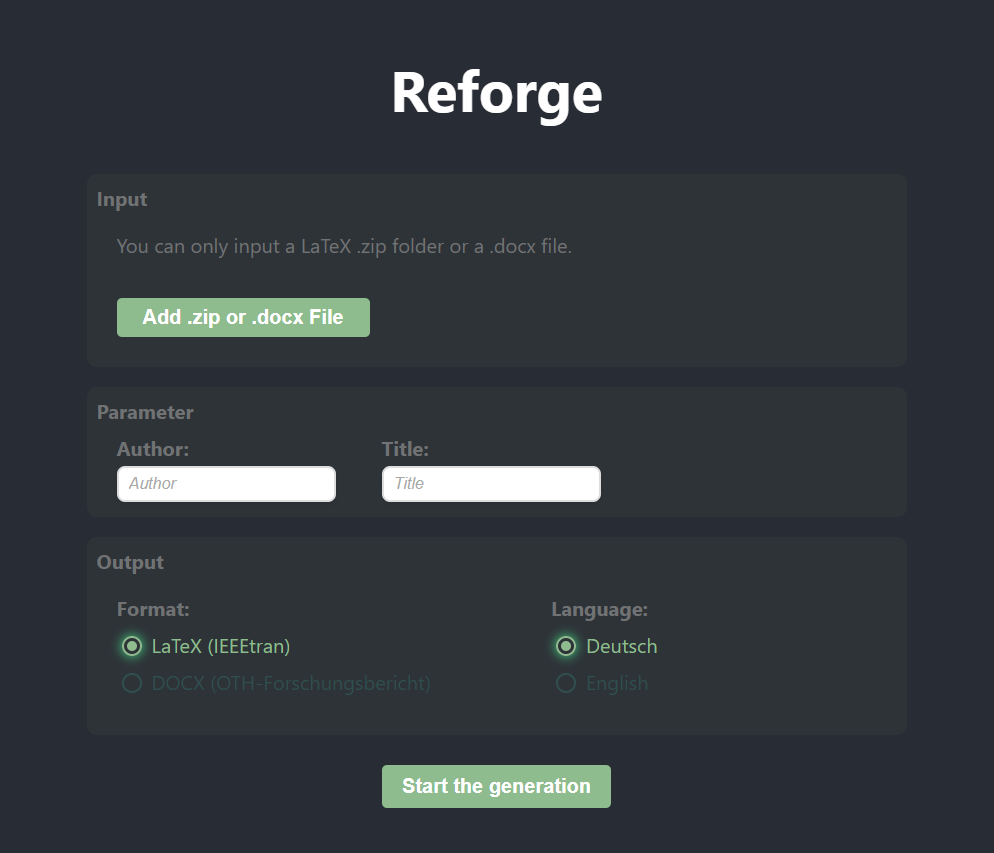
\includegraphics[width=0.9\linewidth]{Images/Frontend Design.png}\\
\caption{Oberflächendesign der Upload-Seite}
\label{fig:Frontend_Design_Upload}
\end{figure}

Die Benutzeroberfläche der Upload-Seite wurde zur besseren Übersichtlichkeit in drei klar definierte Bereiche unterteilt:    
\begin{description}
    \item[Input-Bereich:]
    In diesem Bereich können Dokumente hochgeladen werden, die als Grundlage für die Berichtserstellung dienen. Es werden nur LaTeX-ZIP-Ordner oder \ac{DOCX}-Dateien unterstützt. Diese Einschränkung stellt sicher, dass nur zulässige Dateiformate verarbeitet werden.
    \item[Parameter-Bereich:] 
    Hier werden Parameter wie Autor, Titel und im Falle eines ZIP-Uploads die LaTeX-Hauptdatei eingegeben. Diese Informationen werden für die personalisierte Generierung des Berichts benötigt.
    \item[Output-Bereich:]
    In diesem Bereich kann der Benutzer das gewünschte Ausgabeformat auswählen. Er kann zwischen einer LaTeX- oder einer \ac{DOCX}-Ausgabe entscheiden. Außerdem kann hier die Sprache des Berichts festgelegt werden, wobei der Benutzer nur zwischen Englisch und Deutsch wählen kann.
\end{description}

Die Schaltfläche \textbf{Start the generation} am unteren Rand der Benutzeroberfläche ermöglicht es dem Benutzer, den Prozess der Berichtsgenerierung zu beginnen. Durch die farbliche Hervorhebung ist die Schaltfläche leicht erkennbar und intuitiv zu bedienen.

Die Abbildung \ref{fig:downloadpage} zeigt das Design der Downloadseite. Seit der Erstellung des Wireframes wurden, abgesehen von der Farbgestaltung, keine Änderungen vorgenommen. Lediglich zwei Buttons wurden vorgesehen. Mit \textbf{Download Report} wird der Bericht heruntergeladen und mit \textbf{Generate Another Report} gelangt der Benutzer zurück zur Upload-Seite, falls er einen weiteren Bericht generieren möchte.

\begin{figure}[H]
\centering
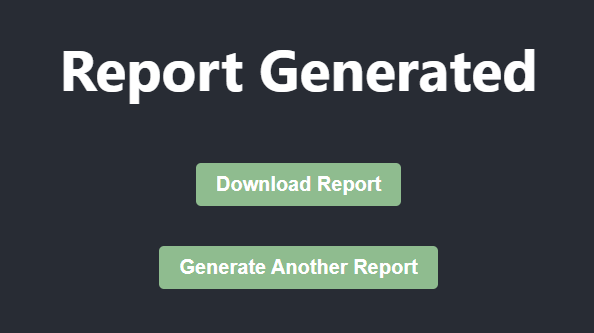
\includegraphics[width=0.5\linewidth]{Images/downloadpage.png}\\
\caption{Oberflächendesign der Download-Seite}
\label{fig:downloadpage}
\end{figure}

Insgesamt wurde bei der Oberflächenentwicklung auf folgendes geachtet:

\begin{description}
    \item[Konsistenz:] Es wurde darauf hingearbeitet, dass die Oberfläche einheitlich ist. Das bedeutet, dass zum Beispiel anklickbare Elemente wie Schaltflächen immer gleich aussehen. So versteht der Benutzer, dass es sich um eine Schaltfläche handelt. Würde man einer Schaltfläche immer wieder eine andere Farbe oder Form geben, wäre dies für den Endnutzer verwirrend. Die Konsistenz hilft, die Bedienung vorhersehbar zu machen.
    
    \item[Feedback und Sichtbarkeit:] Ein weiterer Punkt ist, dem Benutzer ein angemessenes Feedback zu geben, insbesondere wenn er eine falsche Eingabe macht. Wenn der Benutzer beispielsweise vergisst, eine Datei hochzuladen, wird ein Hinweis angezeigt. In diesem Fall werden die Hinweise unterhalb des Start-Buttons angezeigt. Ein Beispiel für eine solche Fehlermeldung ist in Abbildung \ref{fig:Fehleranzeige_Upload} dargestellt. Damit soll der Benutzer bei der Bedienung der Anwendung unterstützt und geführt werden. Sichtbarkeit bedeutet auch, dass der Status des Systems für den Benutzer jederzeit klar sein sollte. Dies wird ebenfalls, wie bei der Fehlermeldung, durch eine Textmeldung an gleicher Stelle erreicht.

    \begin{figure}[H]
    \centering
    
\includegraphics[width=0.8\linewidth]{Images/Frontend_Fehler.png}\\
    \caption{Fehleranzeige auf der Upload-Seite}
    \label{fig:Fehleranzeige_Upload}
    \end{figure}

    \item[Einfachheit und Klarheit:] Die Benutzeroberfläche ist so einfach wie möglich gestaltet. Unnötige Informationen werden vermieden, um den Benutzer nicht zu überfordern. Die Verwendung von klaren Elementen und minimalem Text lenkt die Aufmerksamkeit auf die wesentlichen Funktionen.

    \item[Visuelle Hierarchie:] Durch den gezielten Einsatz von Farben, Größen und Abständen wurde eine klare visuelle Hierarchie geschaffen. Wichtige Informationen oder Aktionen sind hervorgehoben. Dies erleichtert die Orientierung und unterstützt den Benutzer. Auf diese Weise erkennt der Benutzer, was auf der Seite zu erledigen ist. 
\end{description}

Das endgültige Design der Benutzeroberfläche bietet eine klare Struktur, in der die Aufgaben des Benutzers leicht zu verstehen sind. Die gewählten Farben sorgen für eine angenehme visuelle Erfahrung und heben die wichtigsten Aktionen hervor.

\subsection{Die Upload-Seite}
Die Upload-Seite ist, wie bereits erwähnt, dafür verantwortlich, alle für die Berichtsgenerierung notwendigen Informationen an das Backend zu übermitteln. Im Abschnitt \ref{subse:kommu_froback} wurde bereits beschrieben, wie die Kommunikation zwischen Backend und Frontend abläuft. Es wird daher nur auf die zusätzliche Eingabe eingegangen.

Wenn der Benutzer eine ZIP-Datei hochlädt, erscheint ein zusätzliches Eingabefeld. In diesem zusätzlichen Eingabefeld muss der Benutzer den Namen der Hauptdatei des LaTeX-Ordners angeben. Dies wird im Backend dafür benötigt, um die LaTeX-Inhalte in die richtige Reihenfolge zu bringen. Die Abbildung \ref{fig:mainfile_frontend} zeigt, wie das zusätzliche Eingabefeld für die LaTeX-ZIP-Datei aussieht. Wird ein \ac{DOCX}-Dokument hochgeladen, gibt es dieses Eingabefeld für die Hauptdatei nicht, da \ac{DOCX} es nicht benötigt.

\begin{figure}[H]
\centering
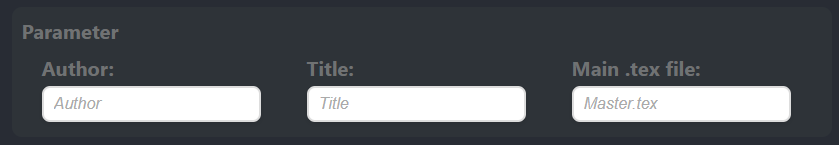
\includegraphics[width=0.8\linewidth]{Images/mainfile_frontend.png}\\
\caption{Das zusätzliche Eingabefeld für die LaTeX-Hauptdatei}
\label{fig:mainfile_frontend}
\end{figure}

\subsection{Die Download-Seite}

Die Download-Seite muss nur die Funktion des Datei-Downloads erfüllen. Die benötigten Daten werden mithilfe des State-Parameters an diese Seite übergeben. Dieser speichert die Zustandsinformationen der aktuellen Seite und ermöglicht deren Übergabe an die Zielseite. Der Wechsel zwischen den Seiten erfolgt über den React Router, der hierfür die Navigate-Funktion nutzt.

Im Listing \ref{lst:state-übergabe} wird der Vorgang der Datenübergabe dargestellt. Dabei wird der React Router verwendet, um die Download-Seite anzusteuern. Der Navigate-Befehl enthält den Zielpfad \texttt{'/download'} und den State-Parameter, der die erforderlichen Informationen wie die Download-\ac{URL}, den Dateititel und das gewünschte Format enthält. Diese Informationen werden anschließend auf der Download-Seite genutzt, um den Download-Prozess auszuführen.

\begin{listing}[H]
\begin{minted}[
frame=lines,
bgcolor=base,
fontsize=\footnotesize,
linenos
]
{typescript}
navigate('/download', { state: { downloadUrl: url, title: title, format: format } });
\end{minted}
\caption{State Übergabe von der Upload-Seite and die Download-Seite}
\label{lst:state-übergabe}
\end{listing}

Der Status der Anwendung wird auf der Download-Seite mit dem \texttt{useLocation}-Hook des React Routers ausgelesen. Die im State enthaltenen Informationen werden über \texttt{location.state} extrahiert. Da das Projekt mit TypeScript umgesetzt wird, müssen die Typen des State-Objekts eindeutig definiert werden. Dies geschieht über das Interface \texttt{LocationState}, welches die Struktur und die Typen der State-Eigenschaften eindeutig beschreibt. Die Implementierung ist im Listing \ref{lst:useLocation} dargestellt.

\begin{listing}[H]
\begin{minted}[
frame=lines,
bgcolor=base,
fontsize=\footnotesize,
linenos
]
{typescript}
import { useLocation } from 'react-router-dom';

interface LocationState {
  downloadUrl: string;
  title: string;
  format: string; 
}

const DownloadPage: React.FC = () => {
  const location = useLocation();
  const { downloadUrl, title, format } = location.state as LocationState;
\end{minted}
\caption{UseLocation-Hook auf der Download-Seite in \textit{Reforge}}
\label{lst:useLocation}
\end{listing}

Um die übergebenen Daten für den Download-Prozess zu verwenden, wird eine Funktion \textbf{handleDownload} implementiert. Diese erzeugt ein temporäres Link-Element, welches die Datei anhand der übergebenen \ac{URL} herunterlädt. Der Dateiname setzt sich dabei aus dem Titel und dem Format der Datei zusammen. Nach dem Klick auf das erzeugte Linkelement wird dieses wieder entfernt, um keine unnötigen Elemente im \ac{DOM} zu hinterlassen. Listing \ref{lst:handleDownload} zeigt, wie diese Funktion realisiert wird. Diese Methode stellt eine Möglichkeit dar, Dateien im Browser herunterzuladen.

\begin{listing}[H]
\begin{minted}[
frame=lines,
bgcolor=base,
fontsize=\footnotesize,
linenos
]
{typescript}
  const handleDownload = () => {
    const link = document.createElement('a');
    link.href = downloadUrl;
    link.setAttribute('download', `${title}.${format}`); 
    document.body.appendChild(link);
    link.click();
    link.remove();
  };
\end{minted}
\caption{HandleDownload-Funktion auf der Download-Seite}
\label{lst:handleDownload}
\end{listing}

  \chapter{Evaluation und Ergebnisse}
In diesem Kapitel werden die Evaluation und die Ergebnisse von \textit{Reforge} vorgestellt. Es beginnt mit einer Beschreibung des Konfigurationsmanagements und der Inbetriebnahme von \textit{Reforge}. Anschließend werden die Kosten für die Nutzung der API analysiert. Die Qualität der generierten Berichte und die mobile Nutzbarkeit werden bewertet. Außerdem wird ein Vergleich der Anwendung \textit{Reforge} mit bestehenden Tools durchgeführt. Abschließend werden die wichtigsten Erkenntnisse und Erfahrungen aus dem Entwicklungsprozess zusammengefasst.

\section{Konfigurationsmanagement und Inbetriebnahme}

Um \textit{Reforge} lokal auszuführen, sind einige Vorbereitungen erforderlich. In diesem Abschnitt wird der Prozess der \ac{API}-Schlüsselgenerierung für OpenAI und DeepL sowie deren Integration in die Anwendung beschrieben.

\subsubsection{Was ist eine \texttt{.env}-Datei?}

Eine \texttt{.env}-Datei ist eine Umgebungsdatei. Sie dient dazu, sensible Konfigurationsdaten wie \ac{API}-Schlüssel, Datenbankzugangsdaten oder andere Umgebungsvariablen sicher zu speichern. Die Anwendung liest die \texttt{.env}-Datei beim Start aus, so dass diese Variablen nicht direkt im Code stehen müssen.

\subsubsection{Die \ac{API}-Schlüsselgenerierung}

Für die Nutzung der OpenAI- und DeepL-\ac{API}s müssen zunächst \ac{API}-Schlüssel generiert werden. Der Prozess beginnt mit der Erstellung eines Benutzerkontos bei den jeweiligen Plattformen. 

Für OpenAI wird die Website \href{https://platform.openai.com}{https://platform.openai.com} besucht, um sich anzumelden oder zu registrieren. Danach wird ein Dashboard sichtbar, über das eine Navigation zu den \ac{API} Keys möglich ist. Nachdem eine Zahlungsmethode hinterlegt wurde, kann dort über \textbf{Create new secret key} ein neuer Schlüssel generiert werden. Es ist wichtig, den Schlüssel direkt zu kopieren und sicher zu speichern, da er nur einmal angezeigt wird.

In ähnlicher Weise erfolgt die Schlüsselgenerierung für DeepL. Es wird die Webseite \href{https://www.deepl.com/pro}{https://www.deepl.com/pro} aufgerufen, um dort einen Account zu erstellen. Anschließend muss auch hier eine Zahlungsmethode ausgewählt werden, womit der Zugriff auf die \ac{API} ermöglicht wird. Im Bereich des Benutzerkontos gibt es einen \ac{API}-Bereich, in dem ein Schlüssel generiert werden kann. Auch hier sollte der Schlüssel sicher gespeichert werden, da er nur einmal erscheint und für die spätere Konfiguration der Anwendung benötigt wird.

\subsubsection{Integration der \ac{API}-Schlüssel in \textit{Reforge}}

Die \textit{Reforge}-Anwendung ist öffentlich auf GitHub verfügbar und kann lokal betrieben werden. Es ist über diesen Link erreichbar: \href{https://github.com/cyberlytics/reforge}{https://github.com/cyberlytics/reforge}

Das Repository muss zunächst in ein lokales Verzeichnis geklont werden. Im Verzeichnis \texttt{sys-src/backend} befindet sich die Datei \texttt{env-example}, die als Vorlage für die Konfiguration der \ac{API}-Schlüssel dient. Um die Anwendung betriebsbereit zu bekommen, müssen die in der Datei enthaltenen Platzhalter durch die zuvor generierten \ac{API}-Schlüssel ersetzt werden.

Der Platzhalter \textbf{dein-openai-api-schluessel} wird durch den \ac{API}-Schlüssel von OpenAI ersetzt, während \textbf{dein-deepl-api-schluessel} mit dem DeepL-Schlüssel überschrieben wird. Anschließend wird die Datei von \texttt{env-example} in \texttt{.env} umbenannt, sodass sie von der Anwendung korrekt eingelesen werden kann. Die resultierende \texttt{.env}-Datei sollte dann wie in Listing \ref{env-api-key} aussehen. Dabei handelt es sich hier um Beispiel-Keys, die nicht funktionsfähig sind und lediglich der Veranschaulichung dienen.

\begin{listing}[H]
\begin{minted}[
frame=lines,
bgcolor=base,
fontsize=\footnotesize,
linenos
]
{csharp}
    OPENAI_API_KEY=sk-12345abcdefghijklmnopqrstuvwxyz12345  
    DEEPL_API_KEY=12345678-90ab-cdef-1234-567890abcdef:fx
\end{minted}
\caption{\texttt{.env}-Datei im sys-src/backend-Ordner}
\label{env-api-key}
\end{listing}

\subsubsection{Inbetriebnahme der Anwendung}

Nachdem die \ac{API}-Schlüssel erfolgreich konfiguriert wurden, müssen die notwendigen Abhängigkeiten installiert werden. Dazu muss der Befehl \textbf{npm install} in einem Terminal in mehreren Verzeichnissen ausgeführt werden. Zuerst im Wurzelverzeichnis, dann im Verzeichnis \texttt{sys-src/backend} und schließlich im Verzeichnis \texttt{sys-src/frontend}. Dieser Schritt stellt sicher, dass alle für die Anwendung benötigten Pakete heruntergeladen und installiert werden.

Nach der Installation der Abhängigkeiten kann die Anwendung gestartet werden. Dazu wird im Terminal in das Verzeichnis \texttt{sys-src/backend} gewechselt und der Backend-Server mit dem Befehl \textbf{npm start} gestartet. Anschließend wird in das Verzeichnis \texttt{sys-src/frontend} navigiert und das Frontend ebenfalls mit \textbf{npm start} ausgeführt. Nach erfolgreichem Start der Anwendung öffnet sich automatisch die \textit{Reforge}-Oberfläche im Browser und steht für die Generierung von technischen Berichten zur Verfügung.

\subsubsection{Hinweise zu möglichen Problemen}

Bei der Nutzung der \textit{Reforge}-Anwendung können unter Umständen Probleme auftreten, die berücksichtigt werden sollten. Zum einen besteht die Möglichkeit, dass die \ac{API}s von OpenAI oder DeepL temporär ausfallen. Solche Ausfälle sind selten, sind aber während der Entwicklungszeit von \textit{Reforge} einmal aufgetreten. In solchen Fällen bleibt nichts anderes übrig, als auf die Behebung der Störung durch die jeweiligen Anbieter zu warten.

Andererseits ist zu beachten, dass die Nutzung der OpenAI-\ac{API} mit Kosten verbunden ist. Diese richten sich nach der Anzahl des verarbeiteten Tokens und variieren je nach Nutzungshäufigkeit und Größe der Anfragen. Eine Aufschlüsselung der entstehenden Kosten ist im folgenden Kapitel \ref{sec:apikosten} beschrieben.

\section{Kosten der API-Nutzung}
\label{sec:apikosten}

Für die Umsetzung der Anwendung wurden die OpenAI und DeepL \ac{API}s genutzt. Die Nutzung dieser \ac{API}s sind mit unterschiedlichen Kosten verbunden, die hier näher erläutert werden.

Die OpenAI \ac{API} bietet verschiedene Preismodelle an, welche auf der Anzahl der verwendeten Tokens basieren. Die Kosten richten sich nach der Anzahl der Ein- und Ausgabe-Token, wobei pro 1.000 Token ein bestimmter Betrag berechnet wird. Für dieses Projekt wurde das \ac{GPT}-3.5-turbo Modell verwendet und zum Zeitpunkt der Entwicklung betrugen die Kosten für \ac{GPT}-3.5-turbo ca. 0,002 US-Dollar pro 1.000 Token. Die tatsächlichen Kosten können je nach Umfang der Anfragen variieren, da längere Dokumente und komplexere Anfragen zu einer höheren Anzahl von Token führen.

Die Abbildung \ref{fig:OpenAI Kosten} zeigt ein Diagramm, welches die Kosten der OpenAI \ac{API} für den Monat August im Jahr 2024 darstellt. Dabei handelt es sich um eine Webseite, auf die zugegriffen werden kann, sobald eine OpenAI \ac{API} verwendet wird. Die Balken, die in der Abbildung zu sehen sind, sind während der Entwicklung von \textit{Reforge} entstanden, als die Anwendung mit Testdaten ausprobiert wurde. Diese Daten können jedoch für eine vorausschauende Kostenanalyse genutzt werden.

\begin{figure}[H]
\centering
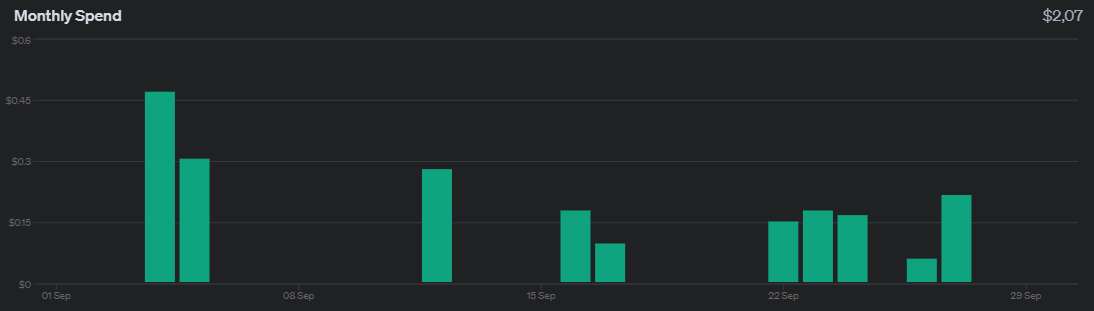
\includegraphics[width=1\linewidth]{Images/MonthlySpend.png}\\
\caption{OpenAI Kosten von August}
\label{fig:OpenAI Kosten}
\end{figure}

Ein weiteres nützliches Diagramm ist in Abbildung \ref{fig:OpenAI Token Usage} dargestellt, welches die Input Tokens und Output Tokens in Relation zu den Kosten zeigt. Aus dem Diagramm geht hervor, dass es sich um Zusammenfassungen handelt, da die Balken für die Output Tokens einen geringeren Ausschlag als die Input Tokens haben. 

\begin{figure}[H]
\centering
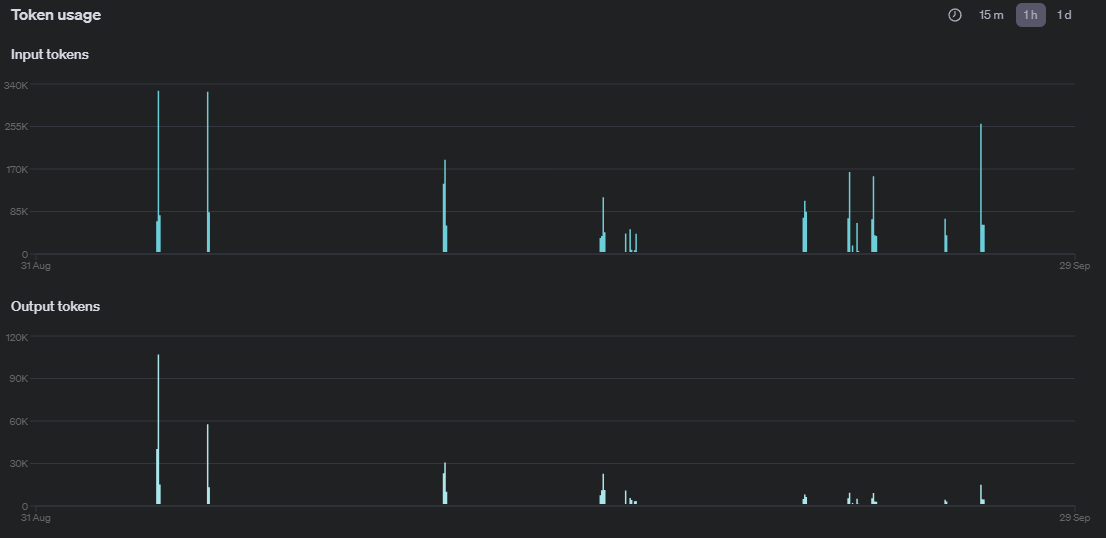
\includegraphics[width=1\linewidth]{Images/TokenUsage.png}\\
\caption{OpenAI Token Usage von August}
\label{fig:OpenAI Token Usage}
\end{figure}

Für den gesamten Entwicklungszeitraum beliefen sich die Kosten für OpenAI auf insgesamt 2,68 US-Dollar. Im August betrugen die Kosten 0,41 US-Dollar, im September 2,07 US-Dollar und im Oktober 0,20 US-Dollar. Insgesamt wurden 118 Berichte generiert, was einem Durchschnitt von ca. 0,023 US-Dollar pro Bericht entspricht. Der Tokenverbrauch zeigt, dass größere Berichte mehr Token und damit höhere Kosten verursachen, während kürzere Dokumente weniger Ressourcen beanspruchen.

Für die DeepL \ac{API} wurde die kostenlose Version verwendet. Diese Version erlaubt eine begrenzte Anzahl an Übersetzungen pro Monat, bietet jedoch eine ausreichende Qualität für die Anforderungen dieses Projekts. Die kostenlose Version ist ideal für kleinere Projekte, da keine direkten Kosten entstehen und dennoch hochwertige Übersetzungen zwischen Deutsch und Englisch möglich sind. Bei einem größeren Umfang oder einer intensiveren Nutzung könnte jedoch eine kostenpflichtige Version erforderlich werden, die zusätzliche Funktionen und ein höheres Übersetzungslimit bietet.

Die Kosten der verwendeten \ac{API}s sind insgesamt überschaubar, insbesondere da die kostenlose Version von DeepL genutzt werden kann. Die OpenAI \ac{API} hingegen verursacht Kosten, die jedoch im Rahmen bleiben und durch die Qualität der generierten Zusammenfassungen gerechtfertigt werden können. Für zukünftige Projekte könnte gegebenenfalls die Nutzung eines anderen OpenAI Modells sinnvoll sein, um das Kosten-Nutzen-Verhältnis weiter zu optimieren.

\section{Qualität der generierten Berichte}

Um die Qualität der erstellten Berichte zu bewerten, wurde ein Bericht auf der Grundlage dieser Arbeit mit \textit{Reforge} produziert. Für die LaTeX-Ausgabe wurde der Bericht in englischer Sprache generiert. Das Ergebnis dieser Generierung ist im Anhang in den Abbildungen \ref{fig:Reforge_testgen1} und \ref{fig:Reforge_testgen2} dargestellt. Zusätzlich wurde eine Generierung für die \ac{DOCX}-Ausgabe durchgeführt. Die Ergebnisse dieser Ausgabe sind ebenfalls im Anhang unter den Abbildungen \ref{fig:ReforgeDOCXGen1} und \ref{fig:ReforgeDOCXGen2} zu finden.

Wie Chang et al. in ihrer Evaluation von \ac{LLM}s beschreiben, neigen \ac{LLM}s in komplexen Kontexten zu Verwechslungen oder Fehlern. Sie stoßen bei der Erkennung semantischer Ähnlichkeiten an ihre Grenzen und zeigen Schwächen in ressourcenarmen Kontexten \cite{10.1145/3641289}. Ob diese Einschränkungen auch hier zutreffen, wurde überprüft. Es zeigte sich, dass Schwächen in ressourcenarmen Kontexten erkennbar sind. Betrachtet man die Abschnitte Bilder und Codeauszüge in den Abbildungen \ref{fig:Reforge_testgen2} und \ref{fig:ReforgeDOCXGen2}, so fällt ein Mangel an Inhalt auf. Dies ist darauf zurückzuführen, dass in diesen Abschnitten kein Text vorhanden ist. Die \textit{Reforge}-Anwendung verarbeitet derzeit keine Bilder und Codeausschnitte, wodurch dieser ressourcenarme Kontext entsteht.

Um die Kompressionsrate $\tau$ von Yadav zu berechnen, wurde die Anzahl der Wörter berücksichtigt \cite{yadav2022automatictextsummarizationmethods}. Diese Arbeit enthält ungefähr 24.150 Wörter. Die Anzahl der Wörter in der generierten \ac{DOCX}-Zusammenfassung \ref{fig:ReforgeDOCXGen1} beträgt ungefähr 970 Wörter. Mit diesen Werten kann nun die Kompressionsrate berechnet werden.

\begin{align}
\mathlarger{\text{0,04017} = \frac{| \text{970} |}{| \text{24.150} |}}
\end{align}

Die Kompressionsrate beträgt somit gerundet 4\% und liegt damit weit unter den gewünschten 15-30\%, die Yadav als gut erachtet. Dies lässt den Schluss zu, dass entweder \textit{Reforge} zu viel Inhalt entfernt oder \ac{GPT}-3.5-turbo zu viel Information auslässt.

Es werden nun die gestellten Fragen aus der Einleitung \ref{einleitung} betrachtet. Zunächst wird untersucht, ob in den generierten Inhalten Biases auftreten. Es zeigt sich, dass das \ac{GPT}-3.5-turbo-Modell keine Biases in den generierten Inhalten aufweist, da es sich ausschließlich auf den Inhalt des hochgeladenen Dokuments stützt.

Die zweite Frage beschäftigt sich damit, ob \textit{Reforge} mithilfe von \ac{KI} bessere Ergebnisse erzielt als ein Mensch. Hier wird deutlich, dass \textit{Reforge} in der Lage ist, eine solide Grundlage zu schaffen. Diese Ergebnisse müssen jedoch von einem Menschen überarbeitet und geprüft werden, sodass \textit{Reforge} die Arbeit des Menschen nicht vollständig ersetzt, sondern lediglich unterstützt.

Abschließend wurde die Frage betrachtet, inwieweit sich die Input-Datei im Vergleich zur Output-Datei verändert. Es konnte festgestellt werden, dass die grobe Inhaltsstruktur erhalten bleibt, während Details teilweise ausgelassen werden. Die weitere Bewertung des erstellten Berichts erfolgte anhand folgender Kriterien.

\begin{itemize}
    \item \textbf{Inhaltliche Genauigkeit:} Die erstellten Zusammenfassungen wurden auf ihre inhaltliche Richtigkeit überprüft. Dabei wurde geprüft, ob die wesentlichen Informationen des Originaldokuments korrekt in die Zusammenfassung übernommen wurden. Die Ergebnisse zeigen, dass das \ac{LLM} in der Lage ist, die wichtigsten Inhalte zusammenzufassen. Da es sich jedoch um eine komprimierte Fassung handelt, gehen Informationen hinsichtlich der Erläuterung der Inhalte verloren.
    \item \textbf{Kohärenz und Lesbarkeit:} Die Berichte sind im Allgemeinen gut lesbar und logisch aufgebaut. Die Verwendung von \ac{LLM} trägt dazu bei, dass die Texte eine natürliche Sprache aufweisen. Dennoch gibt es vereinzelte Fälle, in denen Sätze etwas zu komplex formuliert sind, was die Lesbarkeit beeinträchtigen könnte.
    \item \textbf{Formatierung und Layout:} Ein weiterer wichtiger Aspekt der Evaluierung ist die Formatierung und das Layout der Berichte. Die Anwendung ist in der Lage, vorgegebene Vorlagen wie LaTeX oder \ac{DOCX} korrekt umzusetzen, so dass die resultierenden Berichte den Anforderungen der jeweiligen Vorlage entsprechen.
    \item \textbf{Übersetzungsqualität:} Bei der Evaluierung der Übersetzungsfunktion wurde die Qualität der Übersetzung des generierten LaTeX-Berichts zwischen Deutsch und Englisch untersucht. Das \ac{GPT}-3.5-turbo-Modell erwies sich als zuverlässig. Die Übersetzungen sind im Allgemeinen korrekt und behalten die ursprüngliche Bedeutung des Inhalts bei. Die Titelübersetzungen von DeepL sind ebenfalls richtig.
    \item \textbf{Geschwindigkeit:} Die Erstellung der technischen Berichte dauerte immer weniger als eine Minute und ist somit ein schneller Prozess. Der Zeitaufwand für die Generierung ist im Vergleich zu manuellen Zusammenfassungen minimal.
\end{itemize}

Insgesamt wurde die Qualität der erstellten Berichte als gut bewertet. Die Anwendung erzeugt verständliche technische Berichte und ermöglicht eine korrekte Formatierung. Sie bietet eine gute Vorlage, die manuell ergänzt werden kann.

\section{Evaluation der mobilen Ansicht von \textit{Reforge}}

Die mobile Ansicht der \textit{Reforge}-Anwendung wurde im Browser getestet, um ihre Nutzbarkeit auf kleineren Bildschirmen zu bewerten. Obwohl sich die Webseite für mobile Geräte automatisch skaliert, treten vereinzelt kleinere Layout-Probleme auf. Diese beeinträchtigen jedoch nicht die Funktionalität der Anwendung, sodass die Seite weiterhin vollständig nutzbar bleibt. Die Darstellung der mobilen Version ist in Abbildung \ref{fig:MobileRefUP} zu sehen. \textit{Reforge} erfüllt somit die Anforderungen an Responsive Design. 

\begin{figure}[H]
\centering
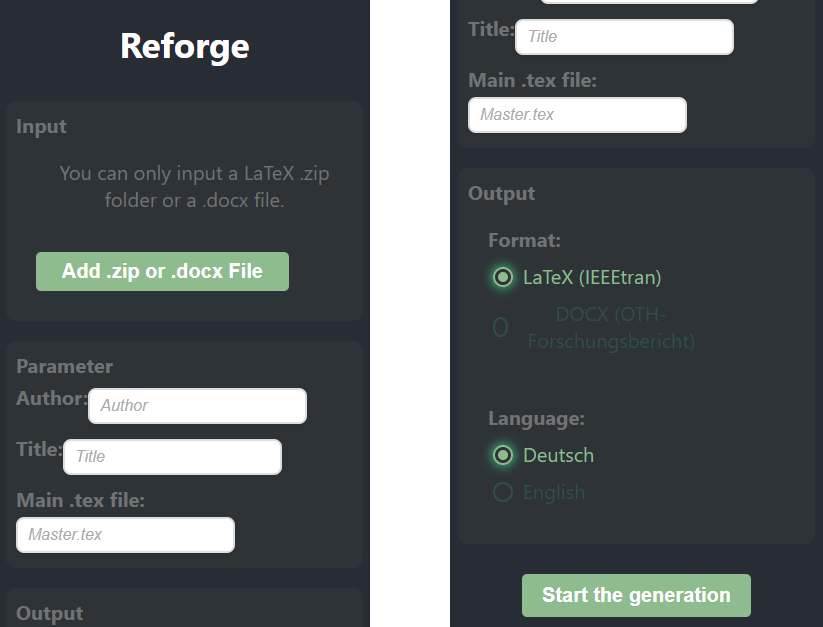
\includegraphics[width=0.8\linewidth]{Images/MobileReforge.png}\\
\caption{Die mobile Ansicht der Upload-Seite von \textit{Reforge}}
\label{fig:MobileRefUP}
\end{figure}

\section{Projektvergleich mit verwandten Webanwendungen}
Um herauszufinden, ob die bestehenden Werkzeuge besser sind als \textit{Reforge}, wird in diesem Abschnitt ein Vergleich mit den verwandten Webanwendungen durchgeführt. Dies soll helfen, den Nutzen von \textit{Reforge} besser einschätzen zu können. 

\subsection{Vergleich mit ChatGPT-4}
Für diesen Vergleich wird versucht, die mit \textit{Reforge} möglichen Ausgaben mit Chat\ac{GPT} zu erzeugen. Dazu wird Chat\ac{GPT} als Eingabe entweder ein \ac{DOCX}-Dokument oder ein LaTeX-ZIP-Ordner übergeben. Zusätzlich wird ein Prompt angegeben, der Chat\ac{GPT} anweist, einen technischen Bericht zu erzeugen. Außerdem wird das Ausgabeformat angegeben, in dem der Bericht erzeugt werden soll. Ähnlich wie bei \textit{Reforge} wird für die LaTeX-Ausgabe IEEEtran und für das \ac{DOCX}-Dokument der OTH-Forschungsbericht angefordert. Um jede Kombination einmal zu testen, werden vier Tests benötigt. Die Ergebnisse der einzelnen Tests sind unten aufgeführt.  Als LaTeX-ZIP-Testdokument für die Generierung wurde die Bachelorarbeit von Hoffmann verwendet \cite{hoffmann_tim_2022bt}. Die Bachelorarbeit von Schotter wurde als Testdokument für die \ac{DOCX}-Generierung verwendet \cite{schotter_tobias_2022bt}.

\subsubsection{Test 1 - LaTeX-ZIP-Ordner zu LaTeX}

Für diesen Vergleich wurde Chat\ac{GPT} gebeten, aus dem LaTeX-ZIP-Archiv eine LaTeX-Ausgabe zu erzeugen. In der Abbildung \ref{fig:Zip_test_anfrage} ist der übergebene Test-Prompt zu sehen. Mit diesem Prompt wurde versucht, Chat\ac{GPT} dazu zu bringen, aus der LaTeX-ZIP-Datei einen technischen Bericht im IEEEtran-Format zu erstellen.

\begin{figure}[H]
\centering

\includegraphics[width=0.8\linewidth]{Images/Zip_test_anfrage.png}\\
\caption{ZIP-Test-Prompt an ChatGPT}
\label{fig:Zip_test_anfrage}
\end{figure}

Chat\ac{GPT} war jedoch nach mehrmaliger Aufforderung nicht in der Lage, das ZIP-Archiv zu analysieren und das gewünschte Ergebnis zu liefern. Es wurde lediglich auf den Inhalt der LaTeX-ZIP-Datei eingegangen und erwähnt, dass die Inhaltsanalyse in Arbeit sei. Die Antwort auf den Prompt ist in der Abbildung \ref{fig:Zip_test_antwort} dargestellt.

\begin{figure}[H]
\centering
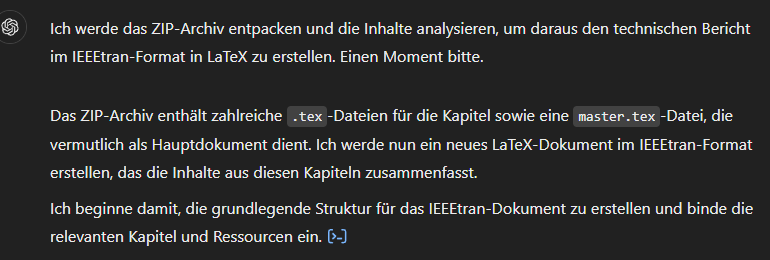
\includegraphics[width=0.9\linewidth]{Images/Zip-test-antwort.png}\\
\caption{ZIP-Test-Antwort von Chat\ac{GPT}}
\label{fig:Zip_test_antwort}
\end{figure}

\subsubsection{Test 2 - DOCX zu LaTeX}

In einem weiteren Test wurde nun das \ac{DOCX}-Dokument an Chat\ac{GPT} übergeben. Dabei war Chat\ac{GPT} in der Lage, eine LaTeX-Ausgabe zu erzeugen, die auch das IEEEtran-Format darstellt. Ein auffallender Nachteil ist jedoch der fehlende Download-Button. Mit Chat\ac{GPT} muss der erzeugte Text manuell kopiert und in eine LaTeX-Datei konvertiert werden, was für den Benutzer zusätzliche Umstände mit sich bringt. Die Chat\ac{GPT} Antwort ist in der Abbildung \ref{fig:docxzulatexgpt} im Anhang dargestellt.

Darüber hinaus gibt es kleinere Fehler in der Ausgabe, wie zum Beispiel die Vermischung von deutscher und englischer Sprache und das Fehlen des Inhalts des Reference-Abschnitts. Dieser Abschnitt müsste bei Bedarf manuell eingefügt werden. Außerdem wurde eine Beispiel-E-Mail eingefügt, die ebenfalls im Nachhinein angepasst werden müsste. Das generierte Ergebnis von Chat\ac{GPT} ist im Anhang in der Abbildung \ref{fig:docxzulatexresult} zu sehen.


\subsubsection{Test 3 - LaTeX-ZIP-Ordner zu \ac{DOCX}}

Es wurde versucht, eine \ac{DOCX}-Ausgabe aus dem LaTeX-ZIP-Ordner zu erhalten. Dazu wurde Chat\ac{GPT} angewiesen, einen technischen Bericht für \ac{DOCX} zu erzeugen. Bei diesem Test erzeugte Chat\ac{GPT} einen Download-Link, um das erstellte \ac{DOCX}-Dokument herunterzuladen. Die Chat\ac{GPT} Antwort auf diesen Test ist in der Abbildung \ref{fig:latexzudocxgpt} im Anhang dargestellt.  

Bei näherer Betrachtung wies das von Chat\ac{GPT} erstellte Dokument zahlreiche Fehler auf, wie die Abbildung \ref{fig:latexzudocxresult} im Anhang zeigt. Die Kapitel sind nicht benannt, sondern durchnummeriert. Außerdem fehlt der obere Rahmen mit Titel, Autor und Studiengang. Ein weiterer Fehler ist, dass LaTeX-Befehle wie Chapter, Section, Cite, Label und Begin im Text vorkommen. Schließlich fehlt der Inhalt des Referenzteils.  

\subsubsection{Test 4 - \ac{DOCX} zu \ac{DOCX}}

Im vierten Test wird probiert, aus dem \ac{DOCX}-Dokument eine \ac{DOCX} Zusammenfassung zu erzeugen. Es wird festgestellt, dass der obere Rahmen wie Autor, Studiengang, Hochschule und Ort fehlt. Außerdem gibt es auch hier keine Referenzsektion. Ein weiteres Problem ist, dass die Ausgabe manuell in eine \ac{DOCX}-Datei eingefügt werden muss. Wie die Chat\ac{GPT}-Ausgabe aussieht, ist im Anhang unter \ref{fig:docxzudocx} zu finden.

\subsubsection{Schlussfolgerung}

Zusammengefasst ist nur Test zwei auf einem ähnlichen Niveau wie die Ausgabe in \textit{Reforge}. Allerdings muss der Benutzer im Dokument von Test zwei die Sprache, die Referenzen und die Daten wie E-Mail überprüfen oder ändern. Alle anderen Tests weisen zu viele Mängel auf, die durch den Anwender korrigiert werden müssten. Andererseits ist anzumerken, dass durch eine Änderung des Prompts möglicherweise bessere Ergebnisse erzielt werden könnten.

Im Vergleich zu Chat\ac{GPT} bietet \textit{Reforge} eine konsistente Ausgabe in Bezug auf Layout und Export. Außerdem muss sich der Benutzer nicht um einen eigenen Prompt bemühen. Er muss lediglich seine Dokumente hochladen und die gewünschten Parameter auswählen. Darüber hinaus achtet \textit{Reforge} auf die Textsprache, so dass es nicht vorkommen kann, dass im Endprodukt eine Mischung aus Englisch und Deutsch erscheint. 

\subsection{Vergleich mit Copilot}
Bei diesem Vergleich wurde zunächst versucht, ein \ac{DOCX}-Dokument in Copilot hochzuladen. Dies wurde jedoch von Copilot mit der Meldung abgelehnt, dass nur Bilder hochgeladen werden können. Diese Mitteilung ist in Abbildung \ref{fig:Copilot_File} dargestellt.

\begin{figure}[H]
\centering
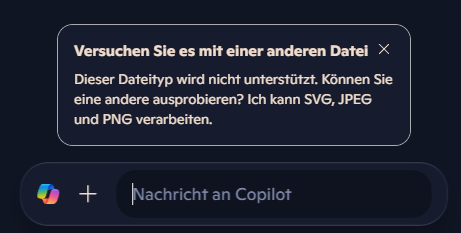
\includegraphics[width=0.7\linewidth]{Images/Copilot_File.png}\\
\caption{Copilot Datei Einschränkungen}
\label{fig:Copilot_File}
\end{figure}

Da ein direktes Hochladen der Datei nicht möglich war, wurde alternativ der Inhalt des \ac{DOCX}-Dokuments kopiert und eingefügt. Dabei stellte sich heraus, dass Copilot ein Zeichenlimit von 10.240 Zeichen vorgibt. Dies ist problematisch, da wissenschaftliche Arbeiten in der Regel deutlich umfangreicher sind. Diese Beschränkung ist in Abbildung \ref{fig:Copilot_Limit} dargestellt. Um Copilot dennoch als Werkzeug für die Berichterstellung nutzen zu können, wäre es notwendig, den Text manuell in kleinere Abschnitte zu unterteilen und diese einzeln zu bearbeiten. Dies würde jedoch einen erheblichen Mehraufwand für den Anwender bedeuten.  

\begin{figure}[H]
\centering

\includegraphics[width=1\linewidth]{Images/Copilot_Limit.png}\\
\caption{Copilot Textlängen Limitierung}
\label{fig:Copilot_Limit}
\end{figure}

Abschließend lässt sich festhalten, dass \textit{Reforge} gegenüber Copilot den Vorteil bietet, dass Dokumente direkt hochgeladen werden können und die Inhalte automatisch in bearbeitbare Abschnitte unterteilt werden. Zudem muss der Benutzer bei \textit{Reforge} keine eigenen Prompts erstellen, da diese bereits vordefiniert sind. Dies vereinfacht die Anwendung und reduziert den Arbeitsaufwand.

\subsection{Vergleich mit Gemini}
Als drittes Vergleichstool wurde Gemini ausgewählt. Ähnlich wie bei Copilot ist das Hochladen von Dateien in Gemini eingeschränkt, wie in Abbildung \ref{fig:Copilot_File} dargestellt. Außerdem muss der Benutzer bei Gemini zusätzlich einen entsprechenden Prompt für die Verarbeitung angeben.

\begin{figure}[H]
\centering
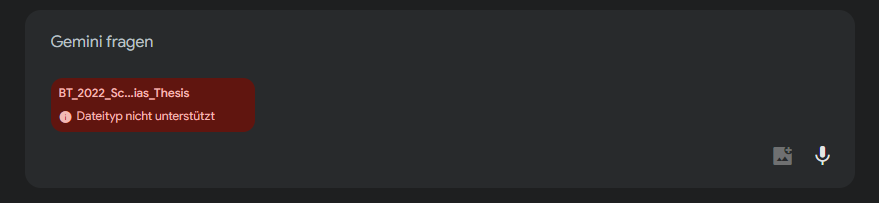
\includegraphics[width=1\linewidth]{Images/Gemini_File.png}\\
\caption{Gemini Datei Einschränkungen}
\label{fig:Gemini_File}
\end{figure}

Stattdessen wurde erneut versucht, den Textinhalt manuell in den Chat einzufügen. Auch hier gibt es jedoch eine Zeichenbegrenzung, ab der das Einfügen weiterer Inhalte nicht mehr möglich ist. Gemini zeigt allerdings keine genauen Informationen über die Zeichenbegrenzung an, was die Arbeit mit längeren Texten erschwert. Um den gesamten Inhalt eines Dokuments verarbeiten zu können, wäre es daher notwendig, den Text manuell in kleinere Abschnitte zu unterteilen.

Im Vergleich zu Gemini zeigt sich, dass der direkte Datei-Upload von \textit{Reforge} den Benutzern viele Arbeitsschritte erspart. Der Textinhalt wird in \textit{Reforge} automatisch in bearbeitbare Abschnitte unterteilt und es sind keine zusätzlichen Eingabeaufforderungen erforderlich.

\subsection{Vergleich mit QuillBot}
Zuletzt wurde \textit{Reforge} mit QuillBot verglichen, einem Tool, das wie \textit{Reforge} keine Chatfunktion bietet. Es dient lediglich zum Zusammenfassen von Texten und unterstützt daher nicht das direkte Hochladen von Dokumenten. Aus diesem Grund muss der Inhalt einer wissenschaftlichen Arbeit für die Zusammenfassung manuell kopiert und eingefügt werden. Es wurde jedoch festgestellt, dass QuillBot eine Begrenzung der Textlänge besitzt, die in Abbildung \ref{fig:Quillbot_Limit} dargestellt ist. Dieses Limit kann durch das Anlegen eines Accounts oder den Erwerb einer Premium-Mitgliedschaft erhöht werden. Diese Abbildung zeigt auch, dass die Zusammenfassung durch die Auswahl von Schlüsselwörtern personalisiert werden kann.  

\begin{figure}[H]
\centering
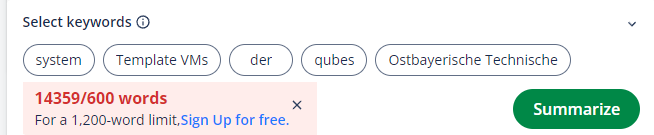
\includegraphics[width=0.8\linewidth]{Images/Quillbot_Limit.png}\\
\caption{Quillbot Textlängen Limitierung}
\label{fig:Quillbot_Limit}
\end{figure}

Weitere Einstellungen, wie beispielsweise die Länge der Zusammenfassung, können ebenfalls in QuillBot vorgenommen werden. Eine Übersicht dieser Einstellungsmöglichkeiten ist in Abbildung \ref{fig:Quillbot_Modes} dargestellt.

\begin{figure}[H]
\centering
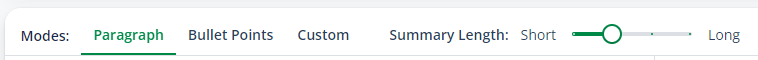
\includegraphics[width=0.8\linewidth]{Images/Quillbot_Modes.png}\\
\caption{Quillbot Einstellugen für die Zusammenfassung}
\label{fig:Quillbot_Modes}
\end{figure}

Zusammenfassend lässt sich festhalten, dass QuillBot aufgrund der Beschränkung der Textlänge nicht mit \textit{Reforge} mithalten kann. Zudem fehlt die Möglichkeit, Dokumente direkt hochzuladen, was eine manuelle Eingabe des Textinhalts erfordert. Andererseits bieten die zusätzlichen Zusammenfassungsoptionen von Quillbot interessante Ansätze. Beispielsweise könnte die Anpassung der Zusammenfassungslänge für zukünftige Versionen von \textit{Reforge} in Betracht gezogen werden.

\section{Lessons Learned}

Die aus Projekten gewonnenen Erkenntnisse werden als Lessons Learned bezeichnet. Patton betrachtet Lessons Learned als lokales, erfahrungsbasiertes Wissen, das oft unspezifisch und ungeprüft ist. Er diskutiert, dass Lessons Learned nicht nur als Methode der Programmevaluierung verwendet werden sollten, sondern auch als Wissensquelle für eine effektive Programmgestaltung \cite{patton2001evaluation}. Im Folgenden wird daher auf die Erkenntnisse eingegangen, die zur Verbesserung zukünftiger Programmkonzeptionen genutzt werden können:

\begin{itemize}
    \item \textbf{Technische Herausforderungen und Lösungsansätze:} Die Integration der OpenAI \ac{API} erwies sich als technisch anspruchsvoll. Dies gilt insbesondere für die Optimierung der Token-Nutzung, um die Kosten gering zu halten. Es wurde gelernt, dass eine sorgfältige Planung der Abfragen und die Aufteilung langer Texte entscheidend ist, um die Tokenbeschränkungen einzuhalten.
    \item \textbf{Bedeutung der Benutzerfreundlichkeit:} Ein weiterer wichtiger Aspekt war die Gestaltung der Benutzeroberfläche. Die Gestaltungsprinzipien erwiesen sich als hilfreich, um die Anwendung auch für Nutzer ohne tiefere technische Kenntnisse zugänglich zu machen. Es wurde deutlich, dass eine klare und einfache Benutzerführung den Umgang mit der Anwendung erleichtert.
    \item \textbf{Kostenmanagement und \ac{API}-Nutzung:} Die monatlichen Kosten für die OpenAI \ac{API} waren überschaubar. Das Projekt hat jedoch gezeigt, dass eine genaue Kostenüberwachung und eine Beschränkung der Anfragen notwendig sind, um im vorgegebenen Budget zu bleiben. Die Nutzung der kostenlosen Version von DeepL war dabei eine sinnvolle Entscheidung, um die Kosten gering zu halten.
    \item \textbf{Zukunftspotenzial:} Während der Entwicklung wurde deutlich, dass die Anwendung durch die Integration weiterer Funktionen noch verbessert werden kann. Diese Erweiterungen bieten Potenzial für zukünftige Projekte und könnten die Anwendungsbreite und den Nutzen von \textit{Reforge} weiter ausbauen. In Kapitel \ref{ch:ausblick} werden mögliche Projekterweiterungen erläutert.
    \item \textbf{Zeitplanung:} Eine gute Zeitplanung ist für die Entwicklung von Anwendungen unerlässlich. Daher ist es wichtig, im Voraus zu überlegen, wie viel Zeit für welche Funktionen aufgewendet werden soll.
\end{itemize}

Die gewonnenen Erkenntnisse bieten wertvolle Einblicke, die in zukünftigen Projekten genutzt werden können.
  \chapter{Projektausblick von Reforge}
\label{ch:ausblick}
In diesem Kapitel werden mögliche Erweiterungen und Verbesserungen für \textit{Reforge} vorgestellt.


\section{Verbesserung der Textbereinigungen}
Ein wichtiger Aspekt bei der Bearbeitung von LaTeX-Dokumenten ist die Textbereinigung. Der derzeitige Ansatz filtert bestimmte Teile der LaTeX-Dateien heraus, um nur den wesentlichen Inhalt zu erhalten. Dies ist notwendig, um die Anzahl der Token für die nachfolgenden Verarbeitungsschritte nicht zu groß werden zu lassen. Allerdings werden dabei auch Codeabschnitte und andere potenziell wertvolle Inhalte herausgefiltert.

In Zukunft könnte eine verbesserte Textbereinigung entwickelt werden, die in der Lage ist, Codeabschnitte in LaTeX korrekt zu erkennen und entsprechend zu behandeln. Damit wäre sichergestellt, dass diese Inhalte nicht verloren gehen und gegebenenfalls in die Zusammenfassung aufgenommen werden können. Insbesondere für wissenschaftliche Arbeiten, die viele mathematische Formeln oder programmiertechnische Elemente enthalten, wäre dies von Vorteil, da so die Zusammenhänge im Text besser erhalten bleiben.

Darüber hinaus sollte die Textbereinigung flexibler gestaltet werden, so dass weitere, bisher ausgeschlossene Inhalte einbezogen werden können. Dies könnte zum Beispiel die Berücksichtigung von Kommentaren umfassen, die zwar derzeit als unwichtig erachtet werden, jedoch für die Interpretation des Textes von Bedeutung sein könnten.

Die Verbesserung der Textbereinigung würde dazu beitragen, eine genauere und vollständigere Zusammenfassung des Originaldokuments zu erstellen. Dies würde auch die Qualität der Berichte verbessern.

\section{Hinzufügen des Literaturverzeichnisses}
Ein weiterer Bereich, der in Zukunft verbessert werden sollte, ist das Literaturverzeichnis. Momentan muss das Literaturverzeichnis manuell hinzugefügt werden, da es nicht automatisch in die generierte Ausgabe übernommen wird. In einer zukünftigen Version der Anwendung sollte das Literaturverzeichnis korrekt erkannt und in das Ausgabeformat integriert werden. Eine automatische Übernahme des Literaturverzeichnisses würde den Generierungsprozess für den Benutzer vereinfachen.

\section{Hinzufügen einer Datenbank}
\label{subsec:datenbank}

Ein möglicher Ansatz zur Verbesserung wäre die Integration einer Datenbank zur Speicherung der Daten. Derzeit werden die Daten nur temporär verarbeitet und nicht dauerhaft gespeichert. Eine Datenbank würde die langfristige Speicherung von Dateien, Metadaten, Bearbeitungsstatus und Benutzerinformationen ermöglichen. Wie Saake et al. betonen, ermöglichen Datenbanksysteme nicht nur die effiziente Speicherung und den Zugriff auf große Datenmengen, sondern gewährleisten auch die Datenunabhängigkeit und die Kontrolle von Mehrbenutzerzugriffen \cite{saake2019datenbanken}. Darüber hinaus wird in ihrem Buch die Implementierung einer Datenbank detailliert beschrieben, welche als wertvolle Grundlage für die Realisierung dienen kann. 

Außerdem hätte die Einführung einer Datenbank mehrere Vorteile. Zum einen könnte der Benutzer jederzeit auf frühere Berichte und Bearbeitungen zugreifen, was die Wiederverwendbarkeit der Ergebnisse begünstigt. Zum anderen könnte eine Datenbank die Verwaltung und Nachvollziehbarkeit der Benutzeraktionen unterstützen, dies wäre insbesondere bei einer größeren Anzahl von Benutzern wichtig. Die Wahl der Datenbanktechnologie wie MongoDB, SQL oder NoSQL würde von den spezifischen Anforderungen des Projekts abhängen.

Die Entwicklung eines konzeptionellen Datenmodells kann ebenfalls Gegenstand künftiger Arbeiten sein. Die Planung eines Informatikprojekts sollte gemäß Vetter systematisch von einer groben zur detaillierten Beschreibung erfolgen. Dabei ist es entscheidend, zunächst eine abstrakte Übersicht des Systems zu erstellen, bevor man sich den spezifischen Details widmet. Ein konzeptionelles Datenmodell bildet dabei die Grundlage für diese Vorgehensweise, da es eine klare Struktur und Orientierung bietet. \cite[S.15 ff.]{vetter2013aufbau}

\section{Berücksichtigung von Bildern}

Ein weiterer Schritt zur Verbesserung der Anwendung könnte die Berücksichtigung von Bildern bei der Verarbeitung sein. Derzeit werden Diagramme, Abbildungen und andere visuelle Inhalte, die oft wichtige Informationen enthalten, herausgefiltert und fehlen somit in der generierten Ausgabe. Dies ist insbesondere für wissenschaftliche Arbeiten von Bedeutung, die häufig auf visuelle Darstellungen zur Veranschaulichung von komplexen Zusammenhängen angewiesen sind.

\section{Erweiterung der Parameter im Frontend}

Eine weitere Verbesserung könnte darin bestehen, dem Frontend mehr Parameter hinzuzufügen, um die Flexibilität der Benutzeroberfläche zu erhöhen. Beispielsweise könnte der Benutzer angeben, welche spezifischen Abschnitte des Dokuments in den Bericht aufgenommen werden sollen. Auf diese Weise könnte der Benutzer den technischen Bericht besser an seine Bedürfnisse anpassen, indem er zum Beispiel nur bestimmte Abschnitte wie die Einleitung, das Fazit oder ausgewählte Kapitel einbezieht. Diese Erweiterung würde dem Benutzer mehr Kontrolle über die generierten Berichte geben.

\section{Asynchrone Verarbeitungen und Benachrichtigungen}

Eine sinnvolle Erweiterung der Anwendung wäre die Option, den fertig generierten Bericht per E-Mail an den Benutzer zu senden. Diese Funktionalität würde es den Nutzern ermöglichen, die Webseite zu verlassen, anstatt auf die Fertigstellung des Berichts zu warten. Besonders bei längeren Verarbeitungszeiten könnte dies die Benutzererfahrung verbessern, da der fertige Bericht automatisch zugestellt wird, sobald die Generierung abgeschlossen ist. 

Eine weitere Möglichkeit der asynchronen Verarbeitung wäre im Kontext einer Datenbank. In diesem Fall könnten die generierten Berichte für jeden Benutzer auf dem Benutzerkonto in der Datenbank gespeichert werden. Auf diese Weise muss der Benutzer auch nicht auf seinen Bericht warten, sondern kann den generierten Bericht später einfach in seinem Account abrufen.

\section{Kostenlimitierung}

Wenn die Anwendung öffentlich zugänglich gemacht wird, sollte im Backend eine Beschränkung implementiert werden, um die Nutzung zu kontrollieren. Diese Beschränkung soll verhindern, dass Nutzer unbegrenzt Dokumente generieren, da dies die Kosten für den Betreiber der Website erheblich erhöhen könnte. Eine solche Maßnahme ist wichtig, damit die Betriebskosten überschaubar bleiben und die Anwendung langfristig nachhaltig betrieben werden kann. 

Eine Möglichkeit wäre, die Anzahl der Berichte, die pro Tag erstellt werden können, auf zwei zu begrenzen. Wenn der Benutzer jedoch mehr als zwei Berichte erstellen möchte, könnte eine Art Kreditsystem eingeführt werden. Mit diesem System könnte der Benutzer mehr Versuche für die Generierung erwerben. Dieses Kreditsystem wird beispielsweise auf Fotor.com verwendet, einer Website für die Erstellung von \ac{KI}-Bildern. Die Abbildung \ref{fig:Fotor_Credits} im Anhang zeigt, wie die Option zum Kauf von Credits auf dieser Webseite aussieht. Darüber hinaus bietet Fotor die Alternative, täglich Credits zu erhalten, so dass der Kauf von Credits nicht zwingend erforderlich ist \cite{fotor}. Ein ähnliches System könnte für \textit{Reforge} durchaus sinnvoll sein, um die Kosten überschaubar zu halten und eventuell einen kleinen Gewinn zu erzielen.

  \chapter{Fazit}

Im Fazit wird die Arbeit abschließend zusammengefasst und die Erreichung der zuvor definierten Ziele reflektiert.

\section{Zusammenfassung der Arbeit}
Im Rahmen dieser Bachelorarbeit wurde die Webanwendung \textit{Reforge} entwickelt und erfolgreich implementiert. Sie ist in der Lage, eingereichte Dokumente zusammenzufassen und in spezifischen Formaten wie IEEEtran oder dem OTH-Forschungsbericht zur Verfügung zu stellen. Besonderes Augenmerk wurde auf die Integration moderner \ac{LLM}s zur Textzusammenfassung und -generierung sowie auf die Unterstützung mehrsprachiger Ausgaben in Deutsch und Englisch gelegt.

Die entwickelte Anwendung bietet Studierenden und Lehrenden eine Plattform zur effizienten Erstellung technischer Berichte. Die Implementierung umfasst sowohl die Verarbeitung von LaTeX-ZIP-Dateien als auch von \ac{DOCX}-Dokumenten. Zudem ermöglicht die Integration von \ac{API}s, wie OpenAI und DeepL, die Textzusammenfassung und Übersetzung.

Die Ergebnisse der Arbeit zeigen, dass der Einsatz von \textit{Reforge} den Zeit- und Arbeitsaufwand reduzieren kann. Das Tool bietet daher eine sinnvolle Anwendungsmöglichkeit und wird dementsprechend als nützlich bewertet. Gleichzeitig wurden die Grenzen der Automatisierung aufgezeigt, wie die Abhängigkeit von Token-Limits und die Notwendigkeit menschlicher Validierung. Diese Arbeit leistet somit einen Beitrag auf dem Gebiet der webbasierten Textzusammenfassung und der Entwicklung von \ac{KI}-Werkzeugen für den akademischen Gebrauch.

\section{Erreichung der Ziele}
In diesem Abschnitt wird dargestellt, inwieweit die gesteckten Ziele und funktionalen Anforderungen des Projekts erreicht wurden. Dabei wird insbesondere auf die in Kapitel \ref{subs:funktionaleAnfoderungen} definierten Anforderungen eingegangen und überprüft, ob diese vollständig umgesetzt wurden. Im Kapitel \ref{kernfragen} wurden drei Kernfragen gestellt, auf die nun Bezug genommen wird. 

Die für die Webanwendung \textit{Reforge} gewählte Architektur erfüllt alle Anforderungen an das System und ermöglicht die Erstellung von TechReports. In dieser Arbeit wurde gezeigt, wie ein \ac{LLM} zur automatischen Textzusammenfassung erfolgreich integriert werden kann. Außerdem wurde die Qualität der generierten Berichte untersucht. Diese entsprechen den Anforderungen und bieten eine Grundlage für manuell erstellte Berichte, sowohl hinsichtlich der Struktur als auch der inhaltlichen Genauigkeit.

Alle in A1 und A2 definierten Anforderungen wurden erfüllt. Die Anwendung ist in der Lage, den gesamten Text der Dokumente zu erfassen und für die Generierung in Segmente zu zerlegen. Diese Segmente werden anschließend fehlerfrei wieder zusammengesetzt. Darüber hinaus funktioniert die Kommunikation mit der OpenAI \ac{API} Schnittstelle. Die generierten Berichte spiegeln zudem den Inhalt des Originaltextes wider.

Die Anforderungen aus A3 \ac{DOCX}- und LaTeX-Output sind ebenfalls vollständig implementiert. Die generierten Berichte werden korrekt im Word- oder LaTeX-Format ausgegeben, wobei spezifische Vorlagen wie IEEEtran oder der OTH-Forschungsbericht berücksichtigt werden.

Die in A4 Multi-lingual definierten Anforderungen werden ebenfalls erfüllt. Der Benutzer kann im Webinterface die gewünschte Sprache für den Bericht auswählen. Die Anwendung generiert den Bericht daraufhin entweder in Deutsch oder Englisch.  

Alle übrigen Anforderungen der A5 sind ebenfalls in \textit{Reforge} berücksichtigt. Die Benutzeroberfläche verfügt über alle geforderten Elemente und ist funktionsfähig. Sowohl der aktuelle Fortschritt als auch Fehlermeldungen der Anwendung werden dem Benutzer angezeigt. Darüber hinaus wurde auch die Funktion zum Herunterladen von Berichten implementiert.

Zusammenfassend kann festgestellt werden, dass alle gesteckten Ziele und definierten Anforderungen erreicht wurden. Die Anwendung ist nicht nur funktionsfähig, sondern ermöglicht auch die Zusammenfassung der Dokumente.
  % ... weitere Kapitel
 
  % Literaturverzeichnis
  \phantomsection
  \addcontentsline{toc}{chapter}{Literaturverzeichnis}
  \bibliographystyle{apalike}
  \bibliography{bibliography.bib}
  \newpage
  
  % Anhang
  \phantomsection
  \addcontentsline{toc}{chapter}{Abbildungsverzeichnis}
  \listoffigures
  \newpage

  \phantomsection
  \addcontentsline{toc}{chapter}{Tabellenverzeichnis}
  \listoftables
  \newpage
  
  \appendix
\chapter{Bilder}
\section{Creditkauf auf Fotor}

\begin{figure}[H]
\centering
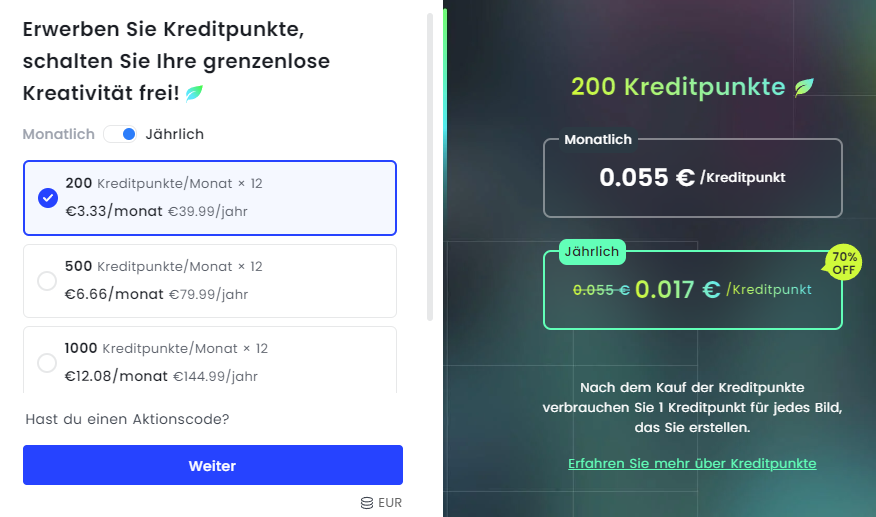
\includegraphics[width=1\linewidth]{Images/Creditkauf auf Fotor.png}\\
\caption{Pop-up Fenster von Fotor.com für den Creditkauf}
\label{fig:Fotor_Credits}
\end{figure}

\section{Reforge LaTeX-Ausgabetest}

\begin{figure}[H]
\centering
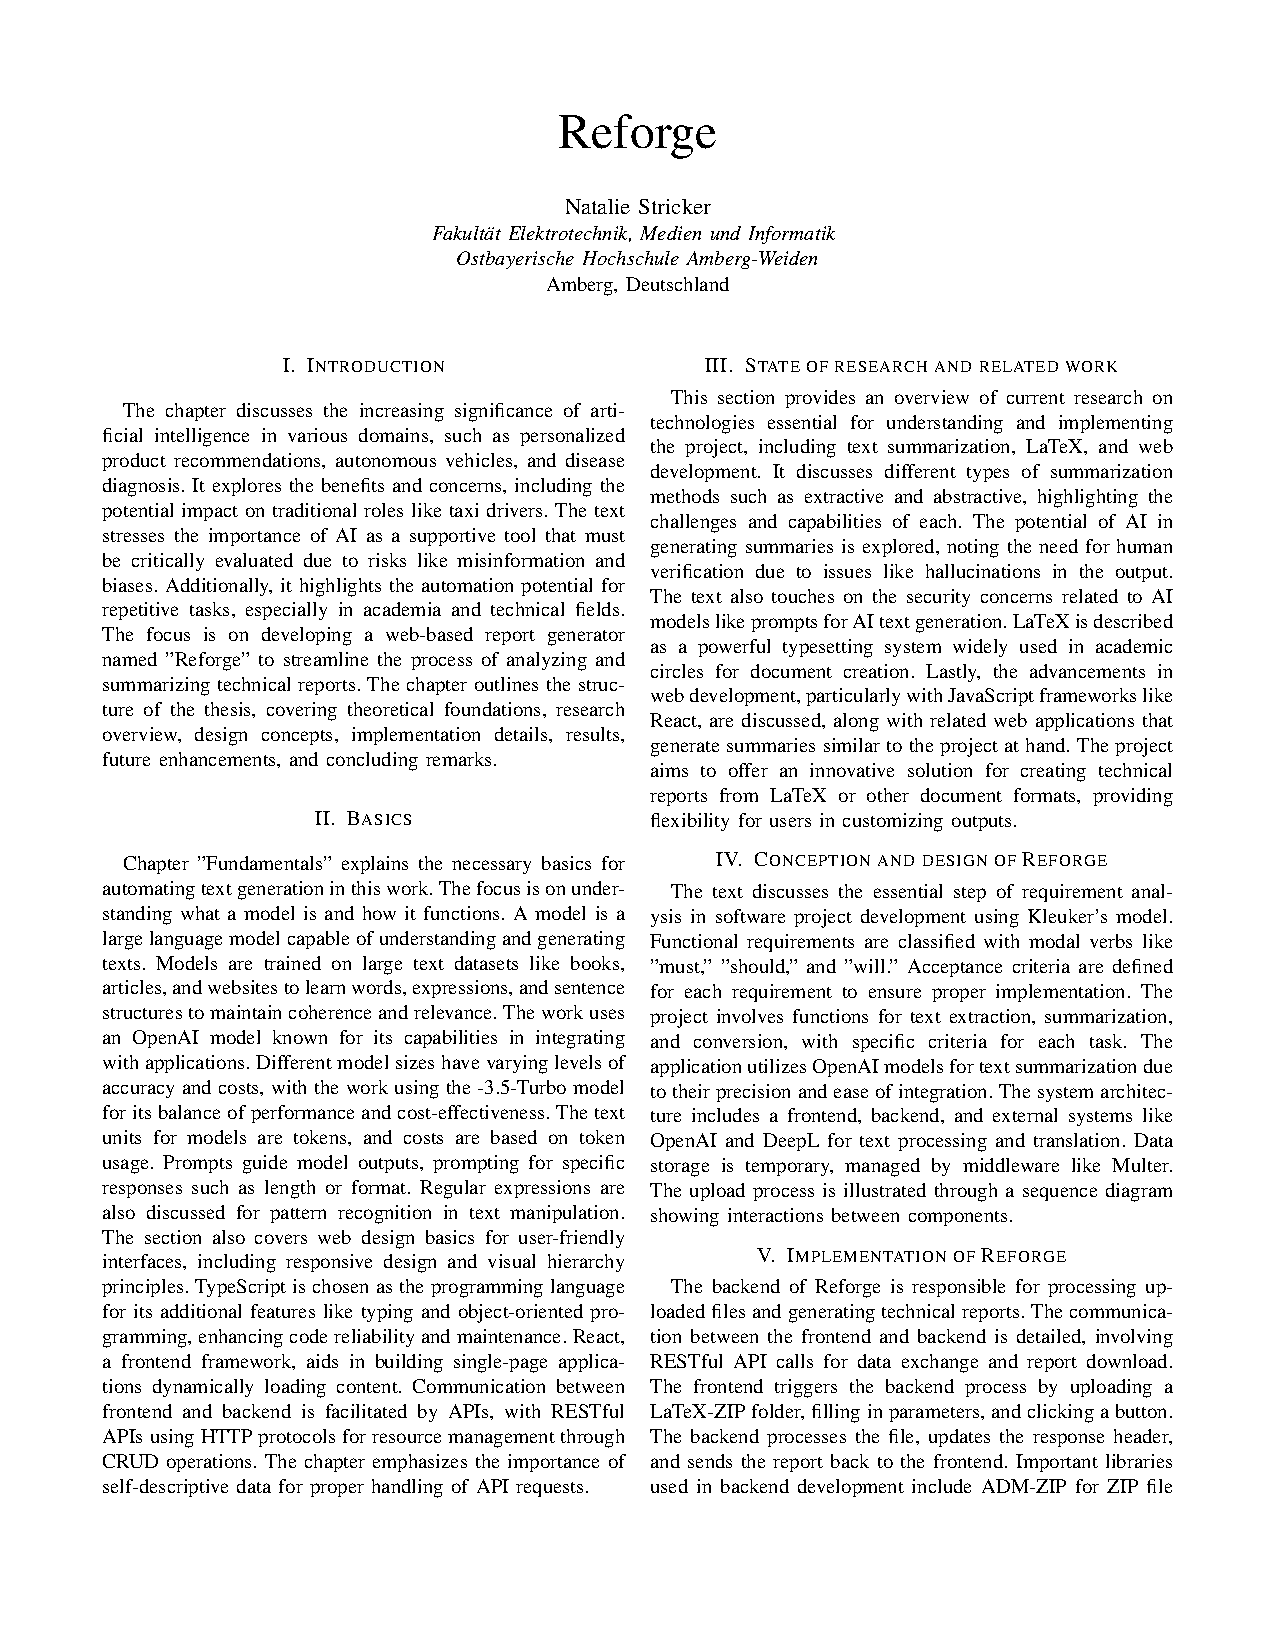
\includegraphics[width=1\linewidth]{Images/ReforgeTestGen1.pdf}\\
\caption{Reforge LaTeX-Ausgabetest auf Basis dieser Bachelorarbeit, Seite eins}
\label{fig:Reforge_testgen1}
\end{figure}

\begin{figure}[H]
\centering
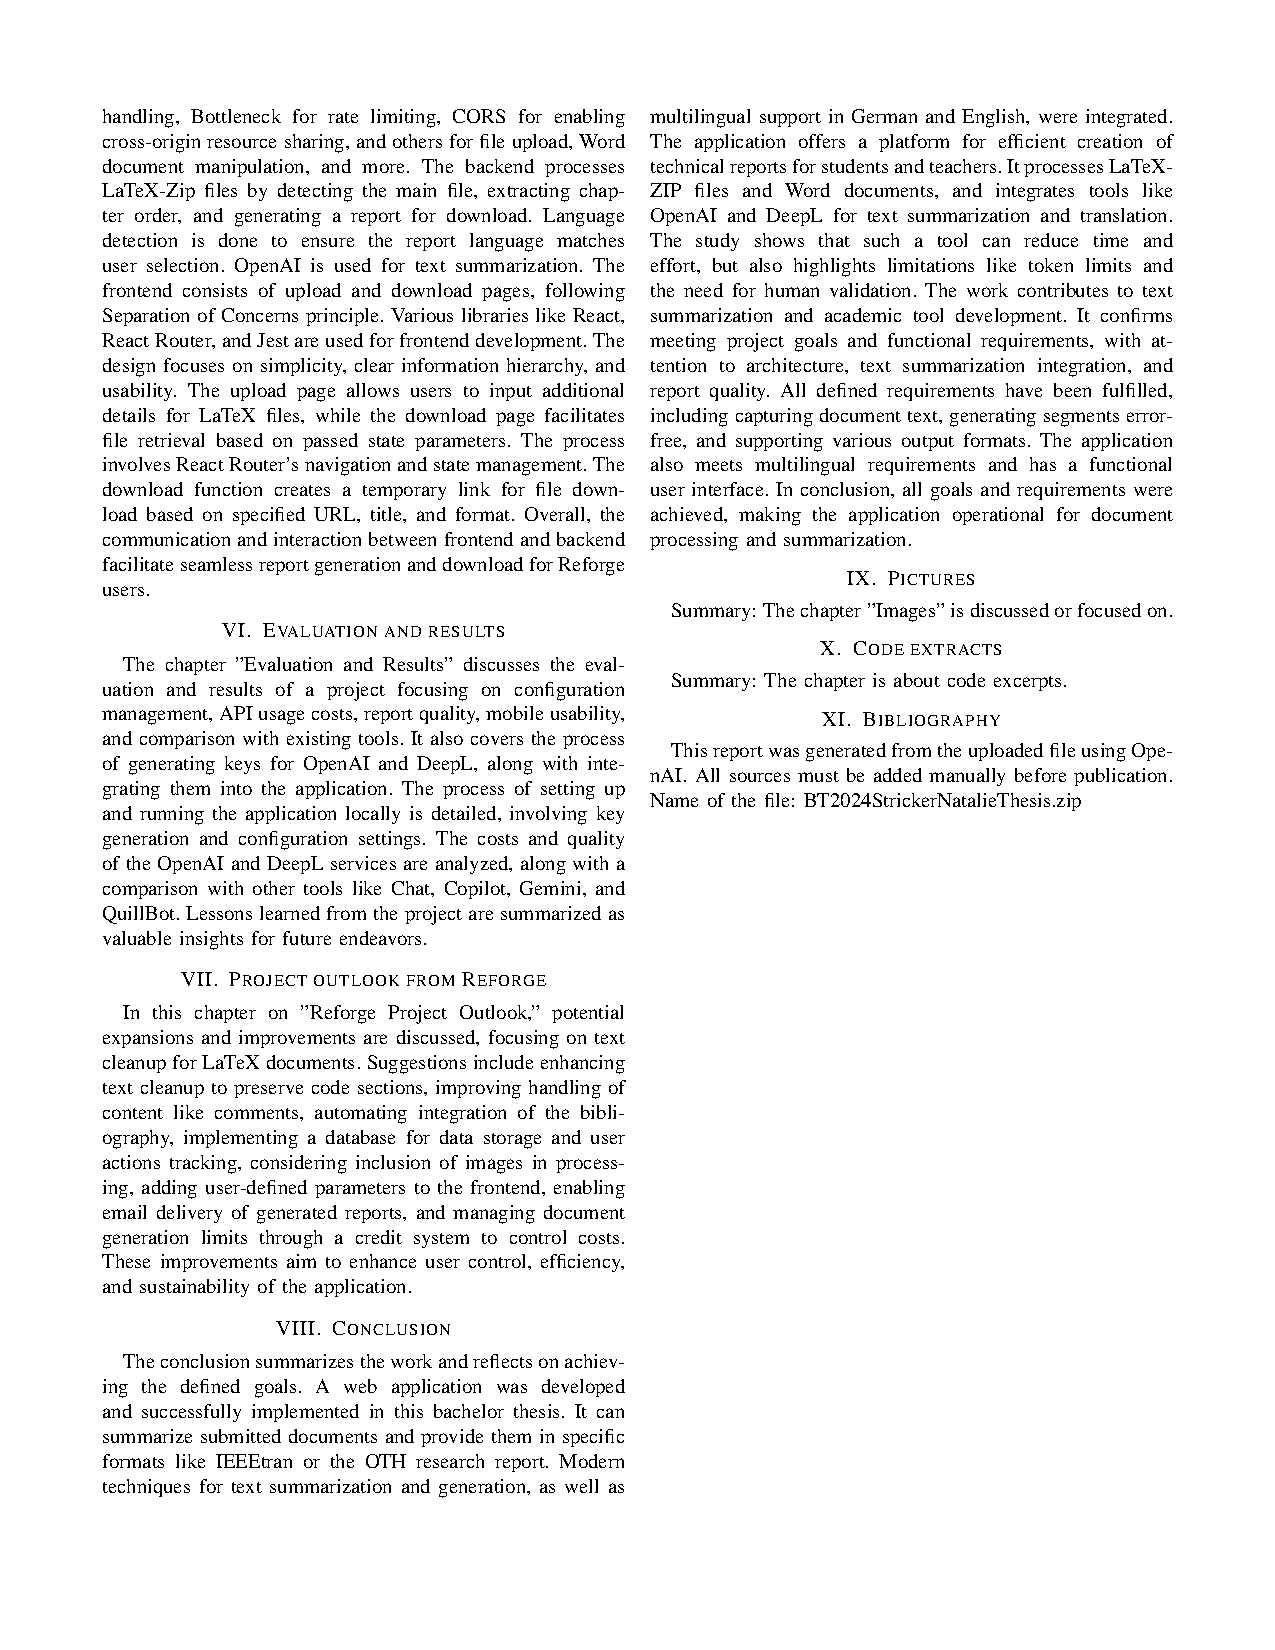
\includegraphics[width=1\linewidth]{Images/ReforgeTestGen2.pdf}\\
\caption{Reforge LaTeX-Ausgabetest auf Basis dieser Bachelorarbeit, Seite zwei}
\label{fig:Reforge_testgen2}
\end{figure}

\section{Reforge DOCX-Ausgabetest}

\begin{figure}[H]
\centering
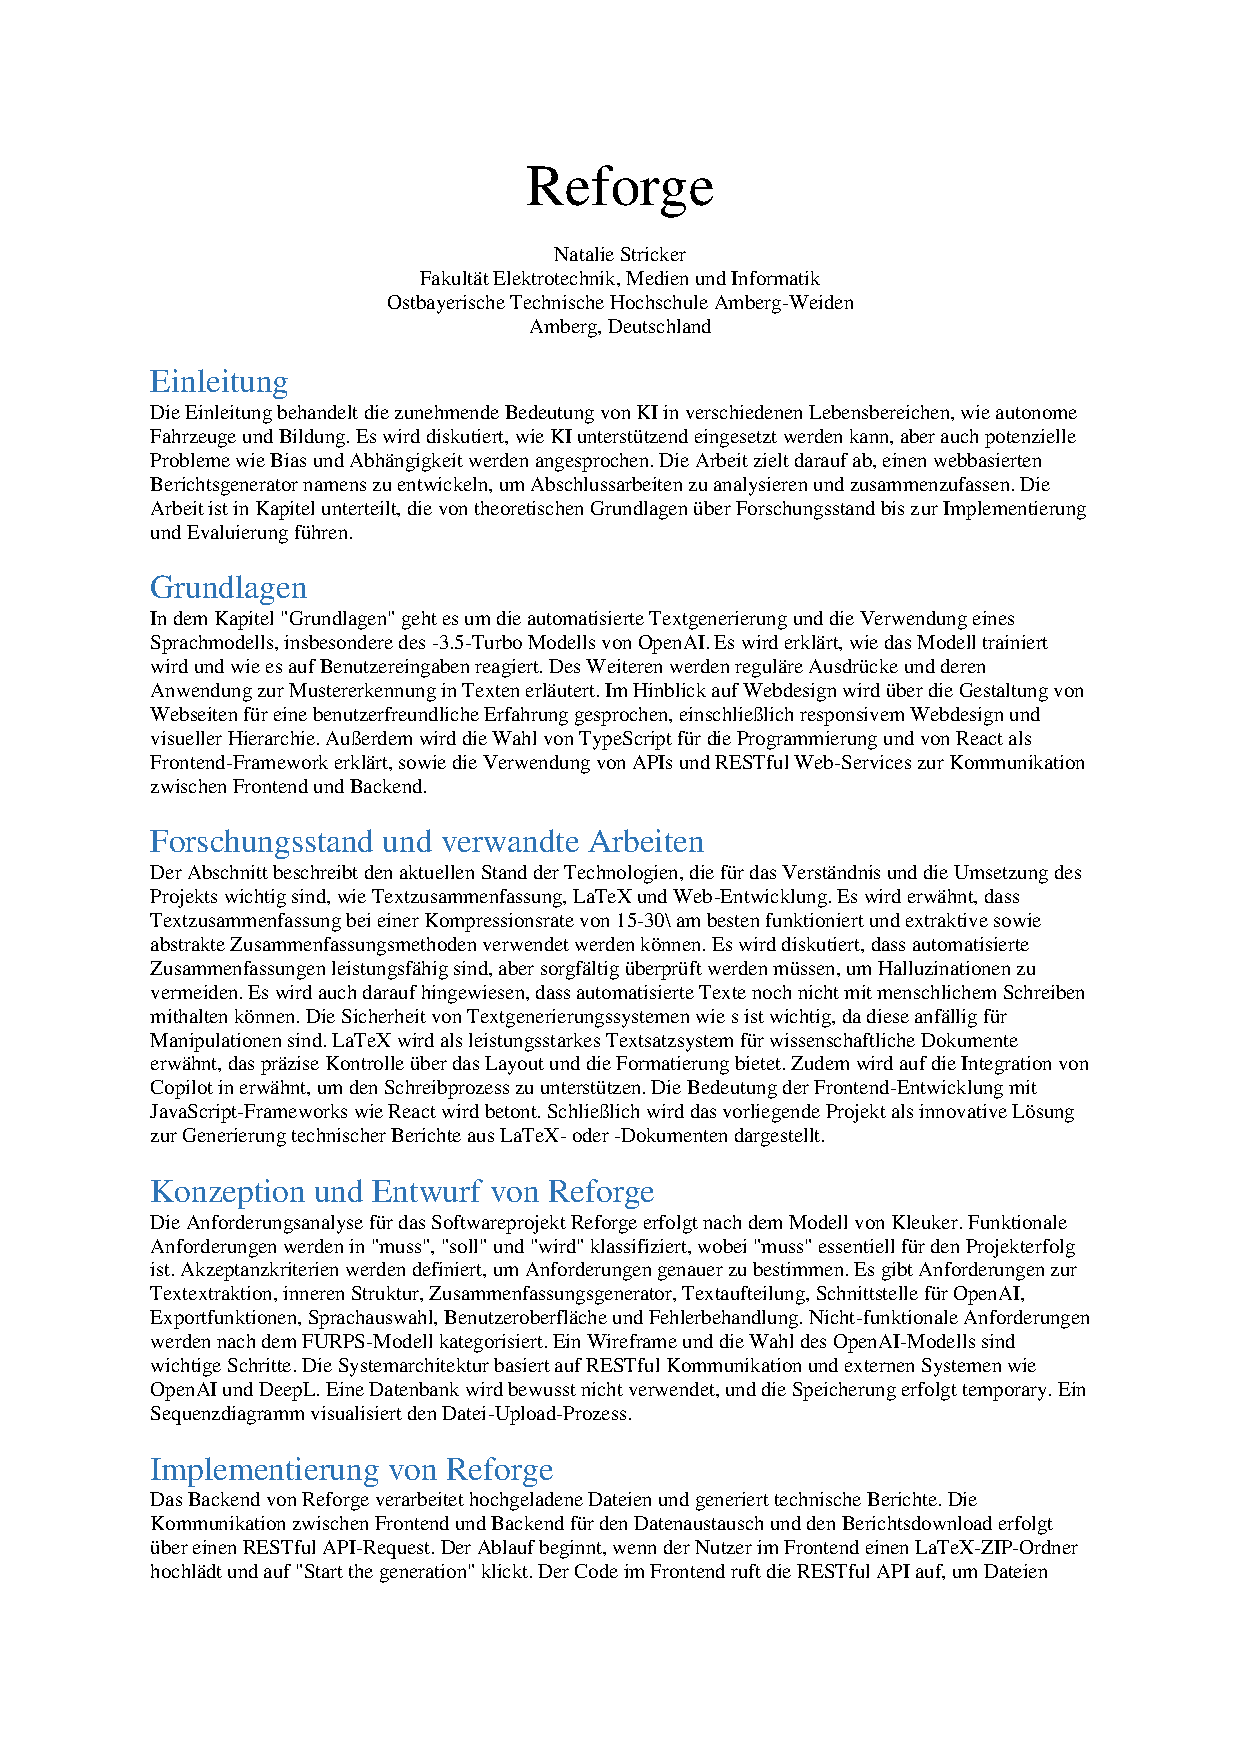
\includegraphics[width=0.9\linewidth]{Images/ReforgeDOCXGen1.pdf}\\
\caption{Reforge \ac{DOCX}-Ausgabetest auf Basis dieser Bachelorarbeit, Seite eins}
\label{fig:ReforgeDOCXGen1}
\end{figure}

\begin{figure}[H]
\centering
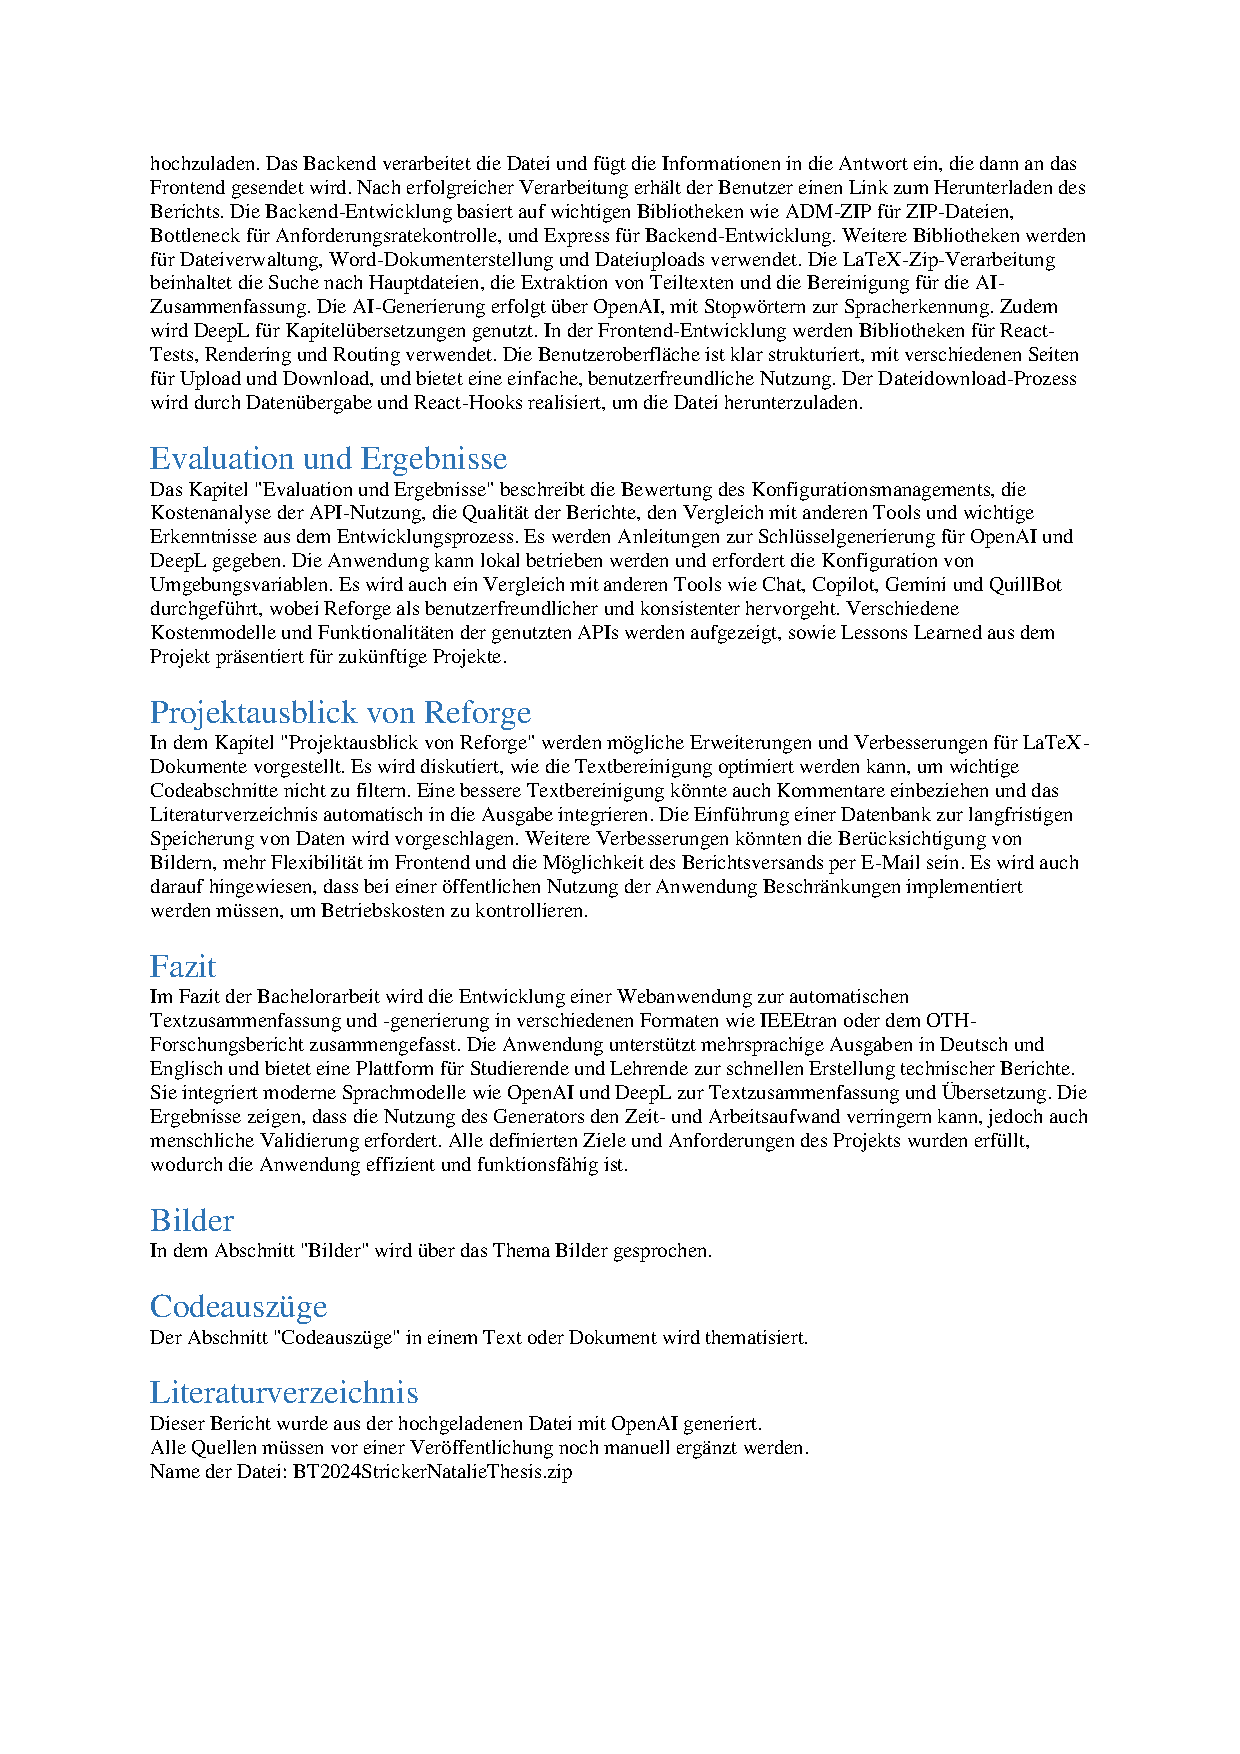
\includegraphics[width=0.9\linewidth]{Images/ReforgeDOCXGen2.pdf}\\
\caption{Reforge \ac{DOCX}-Ausgabetest auf Basis dieser Bachelorarbeit, Seite zwei}
\label{fig:ReforgeDOCXGen2}
\end{figure}

\section{ChatGPT Test 2}

\begin{figure}[H]
\centering
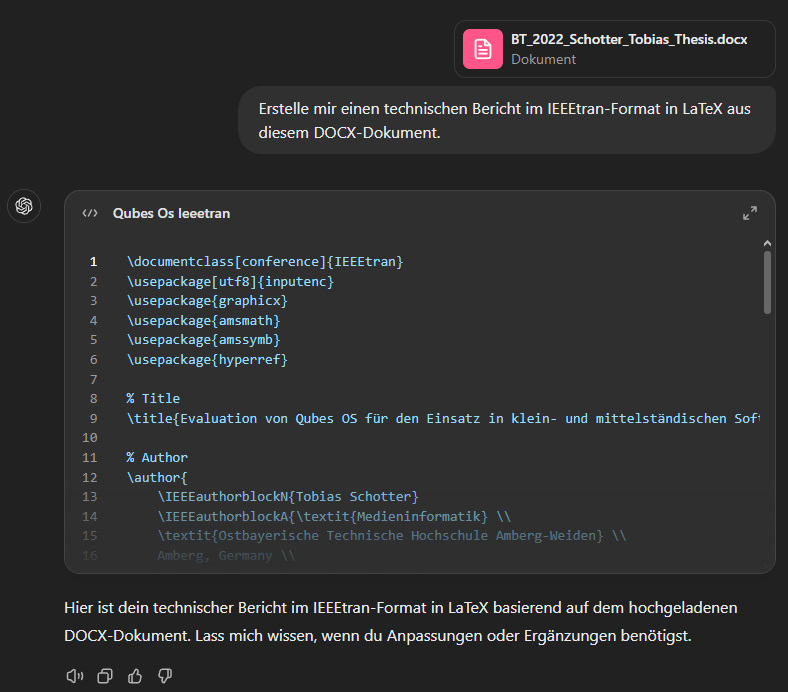
\includegraphics[width=1\linewidth]{Images/DOCXzuLaTeX.png}\\
\caption{Chat\ac{GPT} Test 2: Prompt; Testdokument \cite{schotter_tobias_2022bt}}
\label{fig:docxzulatexgpt}
\end{figure}

\begin{figure}[H]
\centering
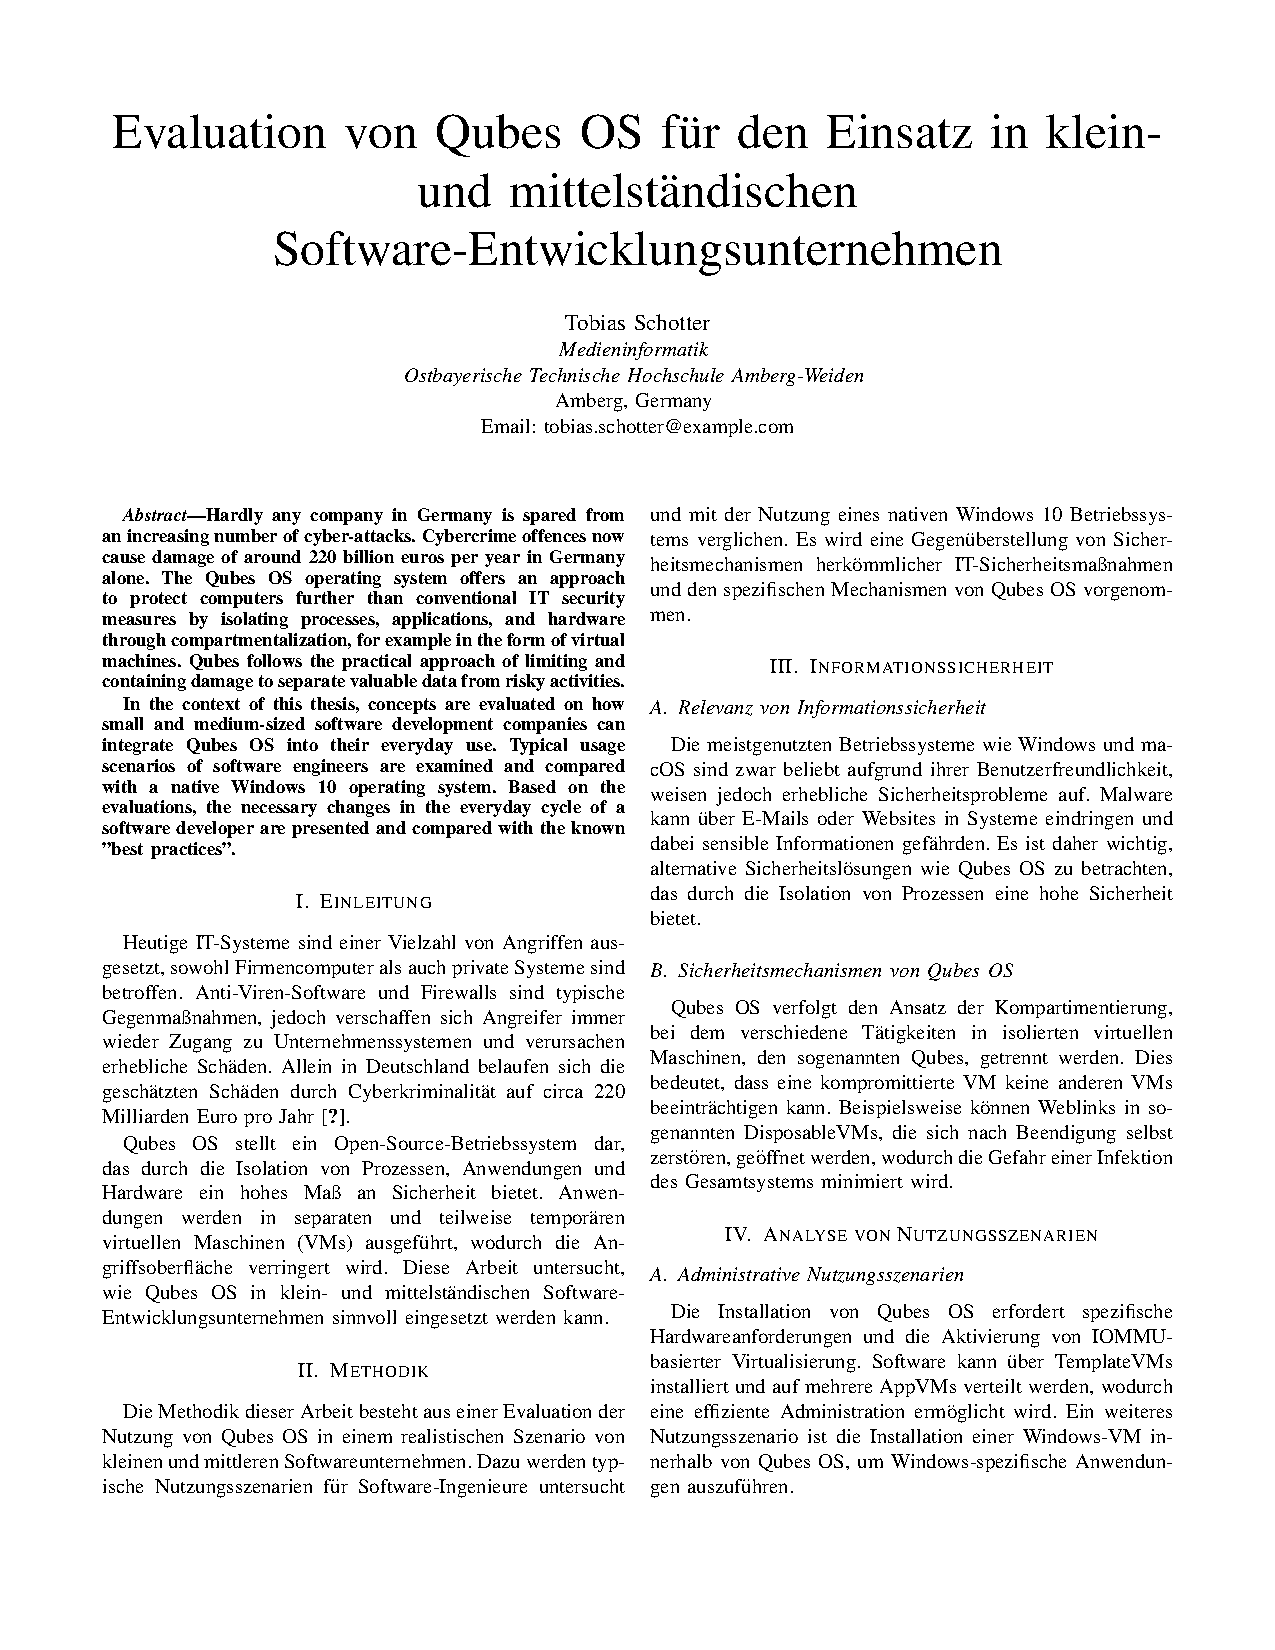
\includegraphics[width=1\linewidth]{Images/docxzulatex.pdf}\\
\caption{Chat\ac{GPT} Test 2: Ergebnis; Testdokument \cite{schotter_tobias_2022bt}}
\label{fig:docxzulatexresult}
\end{figure}

\section{ChatGPT Test 3}

\begin{figure}[H]
\centering
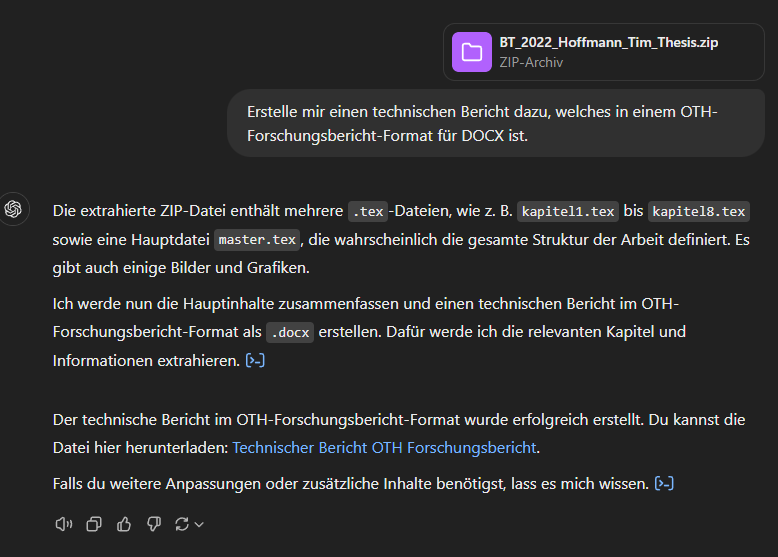
\includegraphics[width=1\linewidth]{Images/ZIPzuDOCX.png}\\
\caption{Chat\ac{GPT} Test 3: Prompt; Testdokument \cite{hoffmann_tim_2022bt}}
\label{fig:latexzudocxgpt}
\end{figure}

\begin{figure}[H]
\centering
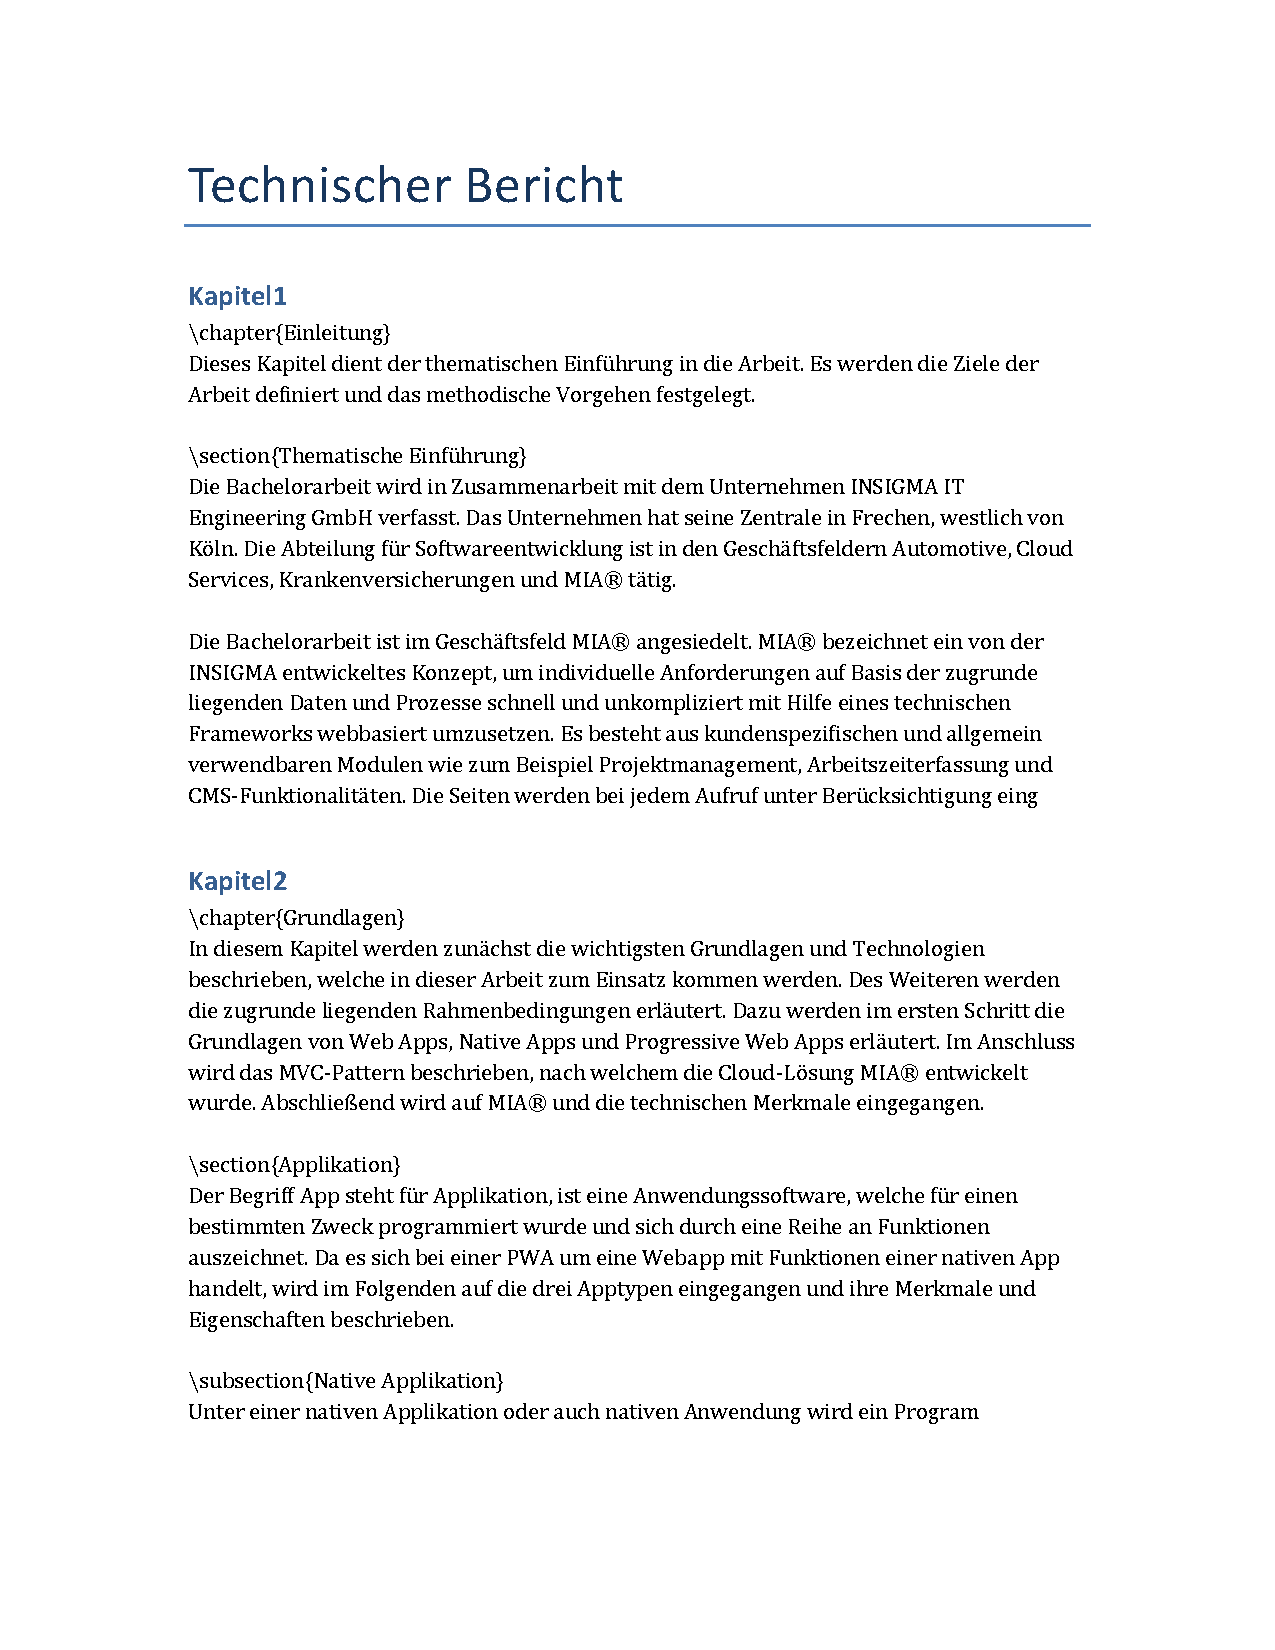
\includegraphics[width=1\linewidth]{Images/chatgpt_oth_forschungsbericht.pdf}\\
\caption{Chat\ac{GPT} Test 3: Ergebnis; Testdokument \cite{hoffmann_tim_2022bt}}
\label{fig:latexzudocxresult}
\end{figure}

\section{ChatGPT Test 4}

\begin{figure}[H]
\centering
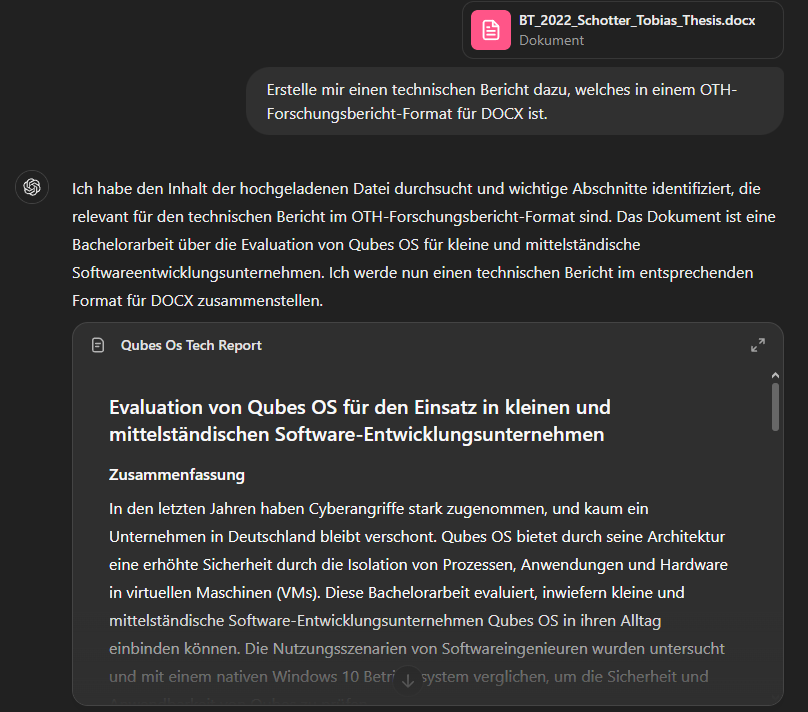
\includegraphics[width=1\linewidth]{Images/DOCXzuDOCX.png}\\
\caption{Chat\ac{GPT} Test 4: Prompt; Testdokument \cite{schotter_tobias_2022bt}}
\label{fig:docxzudocx}
\end{figure}


\chapter{Codeauszüge}

\section{Text-Filterungen}

\begin{listing}[H]
\begin{minted}[
frame=lines,
bgcolor=base,
fontsize=\footnotesize,
linenos
]
{typescript}
export function cleanLatexText(latexContent: string): string {
    // lösche alles vor \chapter{}
    const chapterStartIndex = latexContent.search(/\\chapter\{/);
    if (chapterStartIndex !== -1) {
      latexContent = latexContent.substring(chapterStartIndex);
    }
  
    // Regex für commands
    const commandRegex = /\\[a-zA-Z]+\{[^}]*\}|\\[a-zA-Z]+\[[^\]]*\]|\\[a-zA-Z]+/g;
    // Regex für kommentare
    const commentRegex = /%.*$/gm;
    // Regex für begin & end
    const beginRegex = /\\begin\{[^}]*\}[\s\S]*?\\end\{[^}]*\}/g;
    // Regex für whitespace
    const whitespaceRegex = /\s+/g;
    
    let filteredContent = latexContent
      // Entfernt Kommentare
      .replace(commentRegex, '')
      // Entfernt Begin/End
      .replace(beginRegex, '')
      // Entfernt Commands außer Chapter
      .replace(commandRegex, (match) => {
        return match.startsWith('\\chapter{') ? match : '';
      })
      // Entfernt whitespace
      .replace(whitespaceRegex, ' ')
      .trim();
    
    return filteredContent;
}
\end{minted}
\caption{Funktion für die LaTeX-Text-Filterung}
\label{lst:LaTeX-Text-Filterung}
\end{listing}

\begin{listing}[H]
\begin{minted}[
frame=lines,
bgcolor=base,
fontsize=\footnotesize,
linenos
]
{typescript}
export function removeSpecialChars(section: string): string {
 // entfernt '1.' '2.' etc. am anfang von einer section und special chars
 return section.replace(/\\section\{\d+\.\s*/g,'\\section{').replace(/[&#%_^~$]/g,'');
}
\end{minted}
\caption{Funktion für die SpecialChar-Filterung}
\label{lst:SpecialChar-Filterung}
\end{listing}

\section{DOCX-Dokument Generierung}

\begin{listing}[H]
\begin{minted}[
frame=lines,
bgcolor=base,
fontsize=\footnotesize,
linenos
]
{typescript}
async function PutDocxStyle(title: string, author: string, content: string) {
const doc = new Document({
sections: [
{
properties: {},
children: [
// Titel
new Paragraph({
text: title,
heading: HeadingLevel.TITLE,
alignment: AlignmentType.CENTER,
}),
// Leerzeile
new Paragraph({ text: "" }),
// Autor
new Paragraph({
alignment: AlignmentType.CENTER,
children: [
 new TextRun(author),
 new TextRun({ text: 'Fakultät Elektrotechnik, Medien und Informatik', break: 1 }),
 new TextRun({ text: 'Ostbayerische Technische Hochschule Amberg-Weiden', break: 1 }),
 new TextRun({ text: 'Amberg, Deutschland', break: 1 }),
 ],
}),
// Leerzeile
new Paragraph({ text: "" }),
// Content
...content.split('\n').map((sectionText) => {
 if (sectionText.startsWith('\\section')) {
    return new Paragraph({
     text: sectionText.replace('\\section', '').replace(/[{}]/g, ''),
     heading: HeadingLevel.HEADING_1,
    });
 } else {
    return new Paragraph({
     text: sectionText,
    });
 }
}),
],
},
],
});

 const buffer = await Packer.toBuffer(doc);
 return buffer;
}
\end{minted}
\caption{Generierung eines \ac{DOCX}-Dokuments für die Ausgabe}
\label{lst:docx-gen}
\end{listing}
\end{document}    